\documentclass[twoside,11pt]{article}

% Use JMLR style with preprint option
\usepackage[preprint]{jmlr2e}
\usepackage{amsmath}
\usepackage{bbm} 
% Additional packages (jmlr2e already includes: epsfig, amssymb, natbib, graphicx)
\usepackage{algorithm}
\usepackage{algorithmic}
\usepackage{subcaption}
\usepackage{xcolor}
\usepackage{tikz}
\usetikzlibrary{calc, arrows.meta, decorations.markings, patterns, shapes.geometric, positioning, 3d, decorations.pathmorphing}
\usepackage{array}
\usepackage{tabularx}
\usepackage{listings}
\lstset{basicstyle=\ttfamily, breaklines=true}
\usepackage{booktabs}
\usepackage{xr-hyper}

% Figure search paths (adjust for compilation directory)
\graphicspath{{./}{./figs/}{../}{attention/}{../../Transformer Manuscript/fig_transformer_validation/}}

% Note: jmlr2e already defines theorem, lemma, proposition, corollary,
% definition, example, conjecture, axiom, remark; no manual redefinitions needed.
\newcommand{\softmax}{\operatorname{softmax}}
\newcommand{\KL}{\operatorname{KL}}
\newcommand{\Tr}{\operatorname{Tr}}
\externaldocument[][nocite]{GL(K)_supplementary}
\begin{document}

% JMLR heading for preprint
\jmlrheading{}{2026}{}{}{}{}{Robert C. Dennis}

\title{Attention as Gauge-Theoretic Variational Inference}

\author{\name Robert C. Dennis \email cdenn016@gmail.com \\
  \addr Independent Researcher\\
  \addr Leander, Texas 78641, USA}


\maketitle

\ShortHeadings{Attention as Gauge-Theoretic Variational Inference}{Dennis}
\begin{abstract}
This work constructs an entropy-regularized attention rule as variational inference over transported information sources. Modeling each token as a Gaussian agent on a statistical fiber bundle, we derive the generalized attention weight $\beta_{ij} = \operatorname{softmax}(-D_{\mathrm{KL}}[q_i \| \Omega_{ij} q_j] / \tau)$ from a single variational principle: minimizing the free energy of a mixture-of-sources generative model in which each agent infers, via gauge transport, which neighbor generated its state. The KL divergence arises exactly; the softmax follows from entropy-regularized constrained optimization over the categorical source-selection posterior.

Under specific limits of this principle, standard transformer architectural choices are recovered or structurally compared with the variational geometry: the temperature scaling $1/\sqrt{d_k}$ from dimensional concentration of the KL divergence, layer normalization as a conditional mechanism that can make projected-key norm constancy plausible, multi-head attention as a block-diagonal restriction of the gauge algebra, and causal masking from a hard prior constraint, while ALiBi, T5, and sliding-window positional biases are accommodated as choices of the attention prior $\pi_j$ (the framework fixing the form through which any such prior enters, not the choice itself; see the status taxonomy of Table~\ref{tab:fep_nn_correspondence}). In the strict shared-frame Regime-I reduction, $\Omega_{ij} = I$, and isotropic covariances give the exact logit $\widetilde s_{ij} = \sigma^{-2}\mu_i^\top\mu_j - (2\sigma^2)^{-1}\|\mu_j\|^2$; key-norm constancy then removes the remaining key bias. Layer normalization alone does not enforce this condition after a learned key projection. A general, possibly singular head-space bilinear $M = W_QW_K^\top$ is a separate structural compatibility morphism, not a nonidentity constant Regime-I transport. The individual rectangular projections $W_Q$ and $W_K$ are likewise not gauge transformations.

The contribution is the specific combination of transported Gaussian posteriors, token-local frames, and a $\mathrm{GL}(K)$ entropy-regularized variational construction, together with an ambient full-Gaussian invariance theorem and an iterative diagonal-covariance realization. The empirical evidence retained in the current package is a fixed-$\mathrm{GL}^+(10)$ WikiText-103 width sweep: across three seeds at each of twelve widths, test perplexity decreases from $219.0 \pm 1.3$ at $K=10$ to $74.1 \pm 0.3$ at $K=120$. The 36 runs span ten source commits, so this is a heterogeneous within-sweep development trend rather than a frozen-commit benchmark or a transferable scaling law. It does not establish exact full-$\mathrm{GL}(K)$ equivariance of the realized diagonal-covariance model.
\end{abstract}

\noindent\textbf{Keywords:} gauge theory, free energy principle, transformer attention, variational inference, information geometry, natural gradient, symmetry breaking, multi-agent systems, $\mathrm{GL}^+(K)$ invariance

\section{Introduction}

Language is a dynamic informational system: speakers and writers encode beliefs under uncertainty, listeners decode them, and the statistical regularities of this process reflect the structure of communication itself. Language modeling is a snapshot of this dynamic system, and the architectures that excel at it should reflect the mathematical structure of information exchange under uncertainty.

Recent advances in neuroscience and intelligent systems have independently emphasized the integration of perception, inference, and communication under uncertainty \citep{bahdanau2014neural,amari1998natural,bronstein2021geometric}. Friston's Free Energy Principle (FEP) provides a broad variational formulation of inference in cognitive systems \citep{Friston2010,parr2022active,friston2017graphical,ramstead2020variational}, whereas attention defines a practical rule for token interaction and prediction \citep{clark2019does,vaswani2017attention}. We use the FEP only as variational motivation, independently of the broader and contested general-FEP claims examined by \citet{bruineberg2022emperor}, \citet{aguilera2022particular}, and \citet{biehl2021technical}. The question addressed here is narrower: whether entropy-regularized source selection among gauge-transported Gaussian posteriors yields a specified attention law and which transformer comparisons survive its stated limits.

Many varieties of transformer and attention architectures have been proposed, implemented, and studied \citep{fuchs2020se3,thomas2018tensor}. Geometric deep learning imposes equivariance constraints using group-theoretic structure \citep{cohen2019gauge,kondor2018generalization,finzi2020generalizing,bronstein2021geometric}, while gauge-covariant attention has been engineered for lattice gauge theory through gauge-invariant scores built from Wilson-loop traces of smeared link variables \citep{he2025cask}. Attempts at curved-space token embeddings have produced mixed results \citep{bonnabel2013stochastic,Absil2008}.

Several complementary mathematical perspectives on attention have been developed. \citet{tsai2019transformer} and \citet{katharopoulos2020transformers} analyze attention as a kernel operation, while \citet{ramsauer2021hopfield} identifies the update rule of a modern Hopfield network. The information bottleneck principle \citep{tishby2015deep,shwartz2017opening} supplies a related information-theoretic view of representation learning. Predictive coding \citep{rao1999predictive,bogacz2017tutorial,millidge2021predictive} implements variational free-energy minimization through local prediction errors. These perspectives provide context, but the present construction does not subsume them as consequences of one theorem.

Inference-based attention also has direct precursors. Structured Attention Networks embed graphical-model marginal inference as differentiable attention layers \citep{Kim2017StructuredAttention}. Latent-alignment and variational-attention methods treat attention or alignment as a latent variable \citep{Deng2018LatentAlignment,Bahuleyan2018VariationalAttention}, and Singh and Buckley develop related accounts of attention as implicit structural inference and marginalization \citep{Singh2023ImplicitStructuralInference,Singh2023MarginalProbability}. These works establish that variational or structural readings of attention are not unique to the present model.

Gauge Equivariant Transformer constructs gauge-equivariant multi-head self-attention with parallel transport on triangle meshes \citep{He2021GaugeEquivariantTransformer}, and Energy Transformer defines an explicitly energy-minimizing attention architecture \citep{Hoover2023EnergyTransformer}. Contemporaneous work interprets transformer layers as unrolled inference in probabilistic Laplacian eigenmaps \citep{Ravuri2026UnrolledInference} and develops a free-energy/log-sum-exp mixer \citep{Lu2026FreeEnergyMixer}. These models differ in domain, state space, group action, and objective, but they rule out priority claims for gauge-equivariant attention, energy-minimizing attention, or generic inference and free-energy interpretations of attention.

The closest gauge-theoretic precursor is the proposal that approximate Bayesian inference is itself a gauge theory. \citet{Sengupta2016NeuronalGauge} give a neuronal gauge-theory account, and \citet{sengupta2017gauge} treat posterior parametrization as a local gauge redundancy and use Schild's ladder to parallel transport sufficient statistics, including means and covariances. The distinction is therefore not the presence of geometric transport. It is the token-indexed closed-form vertex transport $\Omega_{ij}=U_iU_j^{-1}$, comparison of transported Gaussian posteriors on an all-pairs token graph, and the restricted reduction toward transformer attention developed here.

The contribution evaluated in this report is the combination of transported Gaussian posteriors, token-local frames, and a $\mathrm{GL}(K)$ entropy-regularized variational construction. Each agent is a local section of an associated bundle with statistical-manifold fibers; the vertex frames define inter-agent transport, and source-selection minimization yields attention from transported KL costs. The scope includes the ambient full-Gaussian invariance theorem and the implemented iterative diagonal-covariance model. It does not include priority for variational attention, latent structural inference, gauge-equivariant attention, energy-minimizing attention, or a generic Gibbs or free-energy interpretation of attention.

We then show that the shared-frame, isotropic Regime-I limit has identity transport and reduces exactly to an identity-bilinear dot-product score plus a key-norm bias. General transformer attention is obtained only after adding the structurally compatible bilinear $M = W_QW_K^\top$. The empirical claim retained here is the fixed-$\mathrm{GL}^+(10)$ development sweep described in Section~\ref{sec:glk_lm} and Supplementary Appendix~J. Supplementary Appendix~E retains the frozen-transformer comparison only as a historical algebraic score check whose design does not support current-release inferential claims.

Finally, we show that the target-blind, Fisher-preconditioned own-row belief update, in the deterministic shared-frame limit with identity transport, has the corresponding message-aggregation structure; the general transformer projections remain structural additions. In filtering mode this is an update map, not certified descent of a global free energy. A fixed likelihood/readout generally reduces the gauge redundancy to the stabilizer of that readout, so the complete free energy is not claimed invariant under the original group. The comparison with training loss plus regularization is structural. The chain rule remains a general property of differentiable function composition; the framework contributes a variational interpretation rather than a derivation of backpropagation.



\begin{figure}[t]
\centering
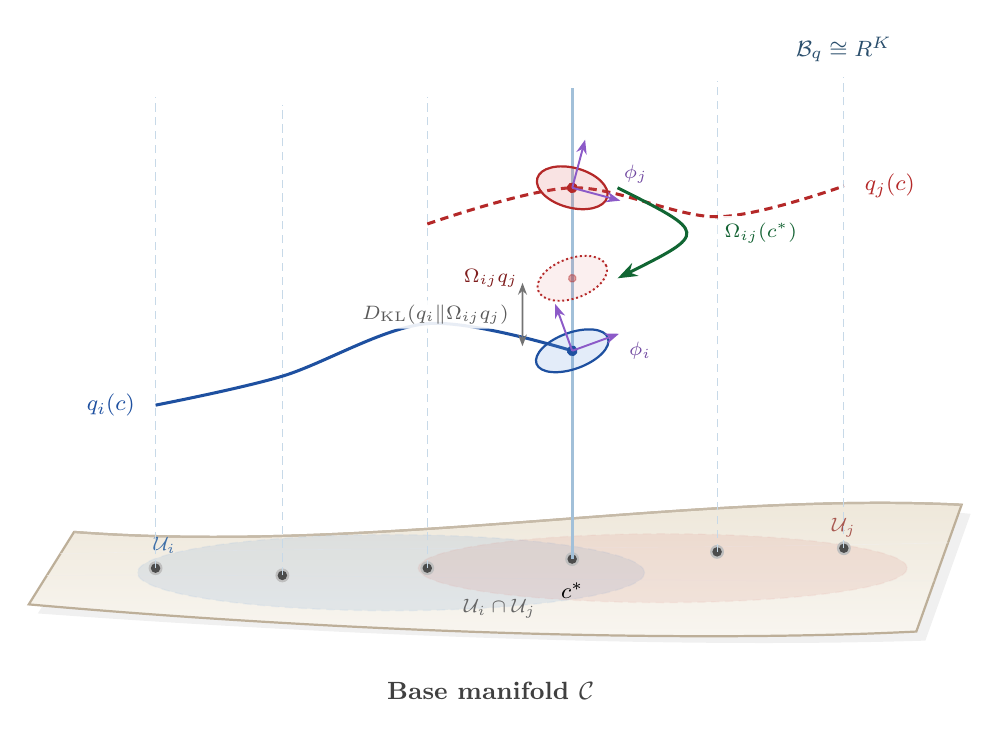
\begin{tikzpicture}[scale=1.15, every node/.style={font=\small}]

% =====================================================================
% COLOR DEFINITIONS
% =====================================================================
\definecolor{fiberblue}{RGB}{70,130,180}
\definecolor{sectionblue}{RGB}{30,80,160}
\definecolor{sectionred}{RGB}{180,40,40}
\definecolor{transportgreen}{RGB}{20,120,60}
\definecolor{gaussblue}{RGB}{100,150,220}
\definecolor{gaussred}{RGB}{220,100,100}
\definecolor{framecol}{RGB}{140,90,200}
\definecolor{basetan}{RGB}{230,220,200}
\definecolor{baseedge}{RGB}{160,140,110}
\definecolor{neighborblue}{RGB}{80,140,210}
\definecolor{neighborred}{RGB}{210,110,100}

% =====================================================================
% BASE MANIFOLD — gently curved surface
% =====================================================================
\path
  (-0.3,0.1) coordinate (M1)
  (9.5,0.4) coordinate (M2)
  (9.0,-1.0) coordinate (M3)
  (-0.8,-0.7) coordinate (M4);

% Shadow
\filldraw[fill=black!6, draw=none]
  ($(M1)+(0.1,-0.1)$)
  .. controls (3.0,-0.2) and (6.5,0.6) .. ($(M2)+(0.1,-0.1)$)
  -- ($(M3)+(0.1,-0.1)$)
  .. controls (6.0,-1.2) and (2.0,-1.0) .. ($(M4)+(0.1,-0.1)$)
  -- cycle;

% Surface fill
\shade[top color=basetan!70, bottom color=basetan!25, draw=baseedge!70, thick]
  (M1)
  .. controls (3.0,-0.15) and (6.5,0.55) .. (M2)
  -- (M3)
  .. controls (6.0,-1.15) and (2.0,-0.95) .. (M4)
  -- cycle;

% Front edge
\draw[baseedge!60, thick]
  (M1) .. controls (3.0,-0.15) and (6.5,0.55) .. (M2);

% Subtle grid lines for depth
\foreach \t in {0.3, 0.6} {
  \draw[baseedge!15, very thin]
  ($(M1)!\t!(M4)$) .. controls
  ($($(M1)!\t!(M4)$)!0.4!($(M2)!\t!(M3)$)+(0,0.04)$) and
  ($($(M1)!\t!(M4)$)!0.6!($(M2)!\t!(M3)$)+(-0.02,-0.04)$)
  .. ($(M2)!\t!(M3)$);
}

\node[below, black!75, font=\small\bfseries] at (4.3,-1.45) {Base manifold $\mathcal{C}$};

% =====================================================================
% FIBER ANCHOR POINTS — six points along the base surface
%
% Layout: C1, C2 in U_i only; C3, C4 in overlap U_i∩U_j;
% C5, C6 in U_j only.
% =====================================================================
\coordinate (C1) at (0.6,-0.30);
\coordinate (C2) at (2.0,-0.38);
\coordinate (C3) at (3.6,-0.30);
\coordinate (C4) at (5.2,-0.20);
\coordinate (C5) at (6.8,-0.12);
\coordinate (C6) at (8.2,-0.08);

% =====================================================================
% LOCAL OPEN NEIGHBORHOODS U_i, U_j ON THE BASE — with overlap
%
% U_i covers C1–C4 (left through overlap).
% U_j covers C3–C6 (overlap through right).
% Overlap region contains C3, C4 — where both sections coexist.
% =====================================================================

% U_i: agent i's local open set (left to center)
% Center at x=3.0 with x-radius 3.0 → right edge at x=6.0, covering C4 at x=5.2
% y-radius 0.35 keeps the ellipse within the base surface (top edge ~y=0.0 here)
\filldraw[neighborblue, opacity=0.12, draw=neighborblue!60,
  line width=0.5pt, densely dashed]
  (3.2,-0.35) ellipse (2.8 and 0.42);
\node[neighborblue!80!black, font=\scriptsize] at (0.7,-0.05) {$\mathcal{U}_i$};

% U_j: agent j's local open set (center to right)
\filldraw[neighborred, opacity=0.12, draw=neighborred!60,
  line width=0.5pt, densely dashed]
  (6.2,-0.30) ellipse (2.7 and 0.38);
\node[neighborred!80!black, font=\scriptsize] at (8.2,0.15) {$\mathcal{U}_j$};

% Overlap label — between C3 and C4
\node[black!60, font=\scriptsize] at (4.4,-0.75) {$\mathcal{U}_i \cap \mathcal{U}_j$};

% Anchor dots
\foreach \c in {C1,C2,C3,C4,C5,C6} {
  \filldraw[black!25] (\c) circle (2pt);
  \filldraw[black!70] (\c) circle (1.3pt);
}

% =====================================================================
% FIBERS — vertical lines rising from each anchor
% =====================================================================
\pgfmathsetmacro{\fh}{5.2}

\foreach \c in {C1,C2,C3,C4,C5,C6} {
  \draw[fiberblue!30, densely dashed, line width=0.4pt]
  (\c) -- ++(0,\fh);
}

% Fiber label (rightmost)
\node[above=2pt, fiberblue!60!black, font=\footnotesize]
  at ($(C6)+(0,\fh)$) {$\mathcal{B}_q \cong \mathbb{R}^K$};

% =====================================================================
% SECTION CURVES — agents i and j as smooth sections of the bundle
%
% CRITICAL: Each section is defined only over its own neighborhood.
% q_i(c) exists over U_i: fibers C1, C2, C3, C4 (blue section)
% q_j(c) exists over U_j: fibers C3, C4, C5, C6 (red section)
% Both sections coexist at C3 and C4 (the overlap U_i ∩ U_j).
% =====================================================================

% Section q_i (blue, solid), defined over U_i only (C1–C4)
\coordinate (Si1) at ($(C1)+(0,1.8)$);
\coordinate (Si2) at ($(C2)+(0,2.2)$);
\coordinate (Si3) at ($(C3)+(0,2.7)$);
\coordinate (Si4) at ($(C4)+(0,2.3)$);

\draw[sectionblue, line width=1.1pt]
  plot[smooth, tension=0.55] coordinates {
  (Si1) (Si2) (Si3) (Si4)
  };

% Section q_j (red, dashed), defined over U_j only (C3–C6)
\coordinate (Sj3) at ($(C3)+(0,3.8)$);
\coordinate (Sj4) at ($(C4)+(0,4.1)$);
\coordinate (Sj5) at ($(C5)+(0,3.7)$);
\coordinate (Sj6) at ($(C6)+(0,4.0)$);

\draw[sectionred, densely dashed, line width=1.1pt]
  plot[smooth, tension=0.55] coordinates {
  (Sj3) (Sj4) (Sj5) (Sj6)
  };

% Section labels — each at the end within its own neighborhood
\node[sectionblue, font=\footnotesize, left=4pt] at (Si1) {$q_i(c)$};
\node[sectionred, font=\footnotesize, right=4pt] at (Sj6) {$q_j(c)$};

% =====================================================================
% HIGHLIGHT FIBER AT c* — at C4, solidly in the overlap U_i ∩ U_j
%
% At this single point c*, BOTH sections q_i(c*) and q_j(c*) live
% in the SAME fiber. The transport Ω_ij(c*) acts WITHIN this fiber
% to align j's frame to i's frame. c* lies in U_i ∩ U_j.
% =====================================================================

% Highlight the fiber at c*
\draw[fiberblue!50, line width=1.0pt] (C4) -- ++(0,\fh);

% Label c* on the base
\node[below=5pt, black, font=\footnotesize\itshape] at (C4) {$c^*$};

% Gaussian ellipses at c* showing beliefs in the same fiber

% q_i(c*): blue Gaussian, frame tilted 20°
\begin{scope}[shift={(Si4)}, rotate=20]
  \filldraw[gaussblue, opacity=0.18] (0,0) ellipse (0.42 and 0.20);
  \draw[sectionblue, line width=0.8pt] (0,0) ellipse (0.42 and 0.20);
  \filldraw[sectionblue] (0,0) circle (1.5pt);
\end{scope}

% q_j(c*): red Gaussian, frame tilted -15° (different gauge frame)
\begin{scope}[shift={(Sj4)}, rotate=-15]
  \filldraw[gaussred, opacity=0.18] (0,0) ellipse (0.40 and 0.22);
  \draw[sectionred, line width=0.8pt] (0,0) ellipse (0.40 and 0.22);
  \filldraw[sectionred] (0,0) circle (1.5pt);
\end{scope}

% Local gauge frames at c* (purple axes)

% Frame for agent i at c*
\begin{scope}[shift={(Si4)}, rotate=20]
  \draw[-{Stealth[length=1.8mm]}, framecol, line width=0.7pt]
  (0,0) -- (0.55,0);
  \draw[-{Stealth[length=1.8mm]}, framecol, line width=0.7pt]
  (0,0) -- (0,0.55);
\end{scope}
\node[framecol!80!black, font=\scriptsize] at ($(Si4)+(0.75,0.0)$) {$\phi_i$};

% Frame for agent j at c*
\begin{scope}[shift={(Sj4)}, rotate=-15]
  \draw[-{Stealth[length=1.8mm]}, framecol, line width=0.7pt]
  (0,0) -- (0.55,0);
  \draw[-{Stealth[length=1.8mm]}, framecol, line width=0.7pt]
  (0,0) -- (0,0.55);
\end{scope}
\node[framecol!80!black, font=\scriptsize] at ($(Sj4)+(0.7,0.15)$) {$\phi_j$};

% =====================================================================
% GAUGE TRANSPORT Ω_ij — acts WITHIN the fiber over c*
%
% At c*, Ω_ij(c*) rotates q_j(c*) from j's local frame into i's
% local frame. Both distributions live in the same fiber; the
% transport is a frame change, not a spatial translation.
% =====================================================================

% Transported ghost: Ω_ij q_j shown near q_i (now in i's frame, dotted)
% Placed 0.8 above q_i, giving space between q_i and ghost
\coordinate (Ghost) at ($(Si4)+(0,0.8)$);
\begin{scope}[shift={(Ghost)}, rotate=20]
  \filldraw[gaussred, opacity=0.10] (0,0) ellipse (0.40 and 0.22);
  \draw[sectionred, densely dotted, line width=0.7pt] (0,0) ellipse (0.40 and 0.22);
  \filldraw[sectionred, opacity=0.4] (0,0) circle (1.2pt);
\end{scope}

% Ghost label — well to the LEFT to avoid green arrow on the right
\node[sectionred!70!black, font=\scriptsize,
  fill=white, fill opacity=0.9, text opacity=1,
  inner sep=1.5pt, rounded corners=1pt, anchor=east]
  at ($(Ghost)+(-0.55,0)$) {$\Omega_{ij} q_j$};

% Transport arrow: curved arc WITHIN the fiber on the RIGHT side,
% from q_j(c*) down to the ghost near q_i(c*).
% Pushed further right (1.4) to clear the ghost label and ellipse.
\draw[-{Stealth[length=2.5mm, width=1.8mm]},
  transportgreen!85!black, line width=1.1pt]
  ($(Sj4)+(0.5,0)$)
  .. controls ($(Sj4)+(1.5,-0.5)$) and ($(Ghost)+(1.5,0.5)$)
  .. ($(Ghost)+(0.5,0)$);

% Transport label — positioned to the right of the arc, well clear
\node[transportgreen!80!black, font=\scriptsize\bfseries,
  fill=white, fill opacity=0.9, text opacity=1,
  inner sep=2.5pt, rounded corners=2pt, anchor=west]
  at ($(Sj4)!0.5!(Ghost)+(1.6,0)$) {$\Omega_{ij}(c^*)$};

% =====================================================================
% KL DIVERGENCE — between q_i(c*) and transported Ω_ij q_j(c*)
% Both distributions are now expressed in agent i's frame
% within the same fiber over c*. Label on the LEFT side.
% =====================================================================

% Double arrow between q_i and the ghost (left side)
\draw[{Stealth[length=1.5mm]}-{Stealth[length=1.5mm]},
  black!55, line width=0.6pt]
  ($(Si4)+(-0.55,0.05)$) -- ($(Ghost)+(-0.55,-0.05)$);

\node[black!65, font=\scriptsize,
  fill=white, fill opacity=0.9, text opacity=1,
  inner sep=1.5pt, rounded corners=1pt, anchor=east]
  at ($(Si4)+(-0.65,0.40)$) {$D_{\KL}(q_i \| \Omega_{ij} q_j)$};

\end{tikzpicture}
\caption{%
Agent belief sections over the associated bundle
$\mathcal{E}_q = \mathcal{N} \times_{\rho_q} \mathcal{B}_q$.
The shaded surface is the base manifold $\mathcal{C}$;
vertical dashed lines are belief fibers $\mathcal{B}_q \cong \mathbb{R}^K$.
Agents $i$ and $j$ each have a local open neighborhood on $\mathcal{C}$:
$\mathcal{U}_i$ (blue, dashed) and $\mathcal{U}_j$ (red, dashed).
Each agent's section is defined only over its own neighborhood:
the blue section $q_i(c)$ exists over $\mathcal{U}_i$,
the red section $q_j(c)$ over $\mathcal{U}_j$.
In the overlap $\mathcal{U}_i \cap \mathcal{U}_j$,
both sections coexist in the same fibers.
At the highlighted fiber over $c^* \in \mathcal{U}_i \cap \mathcal{U}_j$,
$q_i(c^*)$ and $q_j(c^*)$ reside in the same fiber
but are expressed in different local gauge frames
$\phi_i$, $\phi_j$ (purple axes).
The transport operator
$\Omega_{ij}(c^*) = \exp(\phi_i)\exp(-\phi_j)$
(green arrow) acts within this fiber,
rotating $q_j$ from $j$'s frame into $i$'s frame
to produce $\Omega_{ij} q_j$ (dotted red ellipse).
The rotation drawn here is illustrative; a general $\mathrm{GL}(K)$ transport also includes shear and anisotropic scaling, not only rotation.
The attention cost $D_{\mathrm{KL}}(q_i \| \Omega_{ij} q_j)$
is then the divergence between same-frame distributions within a single fiber.
For transformers ($\dim\mathcal{C} = 0$),
all tokens share one base point, the neighborhoods collapse to a single point,
and the entire computation occurs within one fiber.
}
\label{fig:bundle_sections_surface}
\end{figure}


\section{Methods}

We begin with a general geometric construction that naturally supports hierarchical emergence of meta-agents and scale interactions. The details of the most general geometry and framework can be found in the appendix and references \citep{nakahara2003geometry,kullback1951information,sternberg1994group,fulton1991representation,frankel2011geometry,baez1994gauge}.

Briefly, in this current report, we describe agents as modeled by a local section of an associated bundle to a principal $G$ fiber bundle whereby tokens are represented by agents occupying a single 0-dimensional base manifold (Figure~\ref{fig:bundle_sections_surface}). Although the base manifold is 0-dimensional and carries no intrinsic ordering or metric, the discrete index set of agents (tokens) may be endowed with additional structure such as a sequential ordering or a distance function that enters the theory only through the attention prior $\pi_j$ (Section~\ref{sec:nonuniform_priors}) and/or through position-dependent gauge frames (Section~\ref{sec:rope}). This separation between the geometric base (which determines gauge connections and curvature) and the combinatorial index structure (which determines masking and positional biases) is important: causal masking and distance-dependent priors impose structure on which agents communicate, not on the underlying fiber geometry. We shall show that this framework enables a unified description of both intra-agent inference and inter-agent communication in terms of gauge frame transport and alignment via a generalized free energy principle.

\paragraph{Notation and glossary.} Table~\ref{tab:notation} summarizes the principal symbols used throughout this work.

\begin{table}[h]
\centering
\caption{Summary of notation. Symbols are grouped by category: base geometry, agents and beliefs, gauge structure, variational quantities, and Transformer correspondences.}
\label{tab:notation}
\small
\renewcommand{\arraystretch}{1.15}
\begin{tabularx}{\textwidth}{@{}l l X@{}}
\toprule
\textbf{Symbol} & \textbf{Domain} & \textbf{Description} \\
\midrule
\multicolumn{3}{@{}l}{\textit{Base geometry and fibers}} \\
$\mathcal{C}$ & Manifold & Base manifold (spatial domain) \\
$\mathcal{B}_q$ ($\mathcal{E}_q$) & $\mathbb{R}^{K_q}$ & Belief fiber \\
$\mathcal{B}_p$ ($\mathcal{E}_p$) & $\mathbb{R}^{K_p}$ & Model fiber \\
$K$ ($K_q$) & $\mathbb{Z}^+$ & Belief fiber (embedding) dimension \\
$N$ & $\mathbb{Z}^+$ & Sequence length (number of agents) \\
\midrule
\multicolumn{3}{@{}l}{\textit{Agents and beliefs}} \\
$i, j$ & $\{1,\ldots,N\}$ & Agent (token) indices \\
$q_i = \mathcal{N}(\mu_{q,i}, \Sigma_{q,i})$ & $\mathcal{P}(\mathbb{R}^K)$ & Belief distribution of agent $i$ (context-dependent) \\
$p_i = \mathcal{N}(\mu_{p,i}, \Sigma_{p,i})$ & $\mathcal{P}(\mathbb{R}^K)$ & Prior distribution (from token embedding) \\
$s_i, r_i$ & $\mathcal{P}(\mathbb{R}^{K_p})$ & Model-fiber belief and prior (generative model) \\
\midrule
\multicolumn{3}{@{}l}{\textit{Gauge geometry}} \\
$G = \mathrm{GL}(K)$ & Lie group & Structure group (general linear group) \\
$\mathfrak{g} = \mathfrak{gl}(K)$ & Lie algebra & Lie algebra of $G$ \\
$\phi_i \in \mathfrak{g}$ & $\mathbb{R}^{K \times K}$ & Gauge frame parameters for agent $i$ (belief fiber) \\
$\tilde{\phi}_i \in \mathfrak{g}$ & $\mathbb{R}^{K_p \times K_p}$ & Gauge frame parameters for agent $i$ (model fiber) \\
$\Omega_{ij} = \exp(\phi_i)\exp(-\phi_j)$ & $\mathrm{GL}(K)$ & Belief-fiber transport from frame $j$ to frame $i$ \\
$\tilde{\Omega}_{ij}$ & $\mathrm{GL}(K_p)$ & Model-fiber transport from frame $j$ to frame $i$ \\
$\Phi_i, \tilde{\Phi}_i$ & $\mathbb{R}^{K_p \times K_q}$, $\mathbb{R}^{K_q \times K_p}$ & Cross-fiber morphisms (belief $\leftrightarrow$ model); introduced in Supplementary Appendix~A for cross-reference with the companion paper~\citep{Dennis2025it}; not used in any equation of the present paper (see Section~\ref{sec:free_energy_section}) \\
$\rho: G \to \mathrm{GL}(V)$ & & Representation of $G$ on the fiber $V$ \\
\midrule
\multicolumn{3}{@{}l}{\textit{Variational quantities}} \\
$\mathcal{F}$ & $\mathbb{R}$ & Variational free energy; within-channel divergence sector gauge invariant, readout sector gauge fixed \\
$D_{\KL}(q \| p)$ & $\mathbb{R}_{\geq 0}$ & Forward Kullback-Leibler divergence \\
$\beta_{ij}$ & $[0,1]$, $\sum_j \beta_{ij} = 1$ & Belief attention weight (source-selection posterior) \\
$\gamma_{ij}$ & $[0,1]$ & Model-fiber coupling weight \\
$\alpha$ ($\alpha_i$) & $\mathbb{R}^+$ & Prior precision; state-dependent variant (Sec.~\ref{sec:state_dependent_precision}) \\
$\kappa$ ($\tau$) & $\mathbb{R}^+$ & Attention temperature; $\kappa_a$ a $\sigma$-independent per-head sharpness scalar, $\tau_a = \kappa_a\sqrt{d_{\mathrm{head}}}$ (Sec.~\ref{sec:multihead}) \\
$\lambda$ & $\mathbb{R}^+$ & Belief alignment coupling strength \\
$\pi_{ij}$ & $[0,1]$, $\sum_j \pi_{ij} = 1$ & Per-query-row attention prior (encodes masking, positional bias); row index $i$ suppressed in the derivation where it is held fixed \\
$\eta_q, \eta_s$ & $\mathbb{R}^+$ & Belief and model update rates; timescale separation is optional and is not established by the retained same-scale route \\
$\hat\alpha$ & $\mathbb{R}^+$ & Trained-from-loss scalar version of $\alpha$ used in Algorithm~\ref{alg:em_loop} \\
\midrule
\multicolumn{3}{@{}l}{\textit{Transformer correspondences (flat-bundle, isotropic limit)}} \\
$Q_i, K_j$ & $\mathbb{R}^{d_k}$ & Query and key vectors ($\to \mu_i, \mu_j$ under reduction) \\
$V_j$ & $\mathbb{R}^{d_v}$ & Value vector \\
$W_Q, W_K$ & $\mathbb{R}^{d_k \times d}$ & Projection matrices (the product $M = W_QW_K^\top$ is a structural compatibility morphism, not Regime-I transport) \\
$d_k$ & $\mathbb{Z}^+$ & Head dimension ($= K$ per irrep block) \\
\bottomrule
\end{tabularx}
\end{table}

\subsection{An intuitive simplification for non-geometers}
For interdisciplinary readers, it may be helpful to visualize each agent in this framework as a vector and a matrix field defined over a finite spatial region. 

Concretely, at every point $c$ in the base manifold, agent $i$ carries a mean vector $\mu_i(c)$ and a covariance matrix $\Sigma_i(c)$ representing, respectively, its local expected state and uncertainty. Together these form a smooth Gaussian field—the agent’s belief section of the statistical bundle. 

We will see that the agent's local gauge frame $\phi_i(c)$ may be intuitively interpreted as the agent's subjective frame of reference; its internal coordinate system through which beliefs and models are represented and compared. In this sense, $\phi_i(c)$ captures an agent’s “internal orientation” toward the world: it determines how external information is projected into the agent’s internal representational space. Gauge transformations $\phi_i(c) \to \phi_i(c) + \xi(c)$ thus correspond to changes in perspective that leave the underlying informational content invariant, much like shifts of viewpoint in perception that preserve the same world model.\footnote{The additive form $\phi_i \to \phi_i + \xi$ is the abelian (infinitesimal, commuting) linearization. For nonabelian $\mathrm{GL}(K)$ the exact transformation acts multiplicatively on the frame, $U_i = \exp(\phi_i) \to g U_i$. The coordinate expression $\phi_i \to \log(g\exp(\phi_i))$ is valid only locally where the product lies in a real-logarithm chart; it is not a global action on single-exponential coordinates. For example, $\operatorname{diag}(-1,-2)\in\mathrm{GL}^+(2)$ has no real matrix logarithm. Where the chart exists, Baker-Campbell-Hausdorff commutator corrections apply, while the group-valued edge law $\Omega_{ij} \to g_i \Omega_{ij} g_j^{-1}$ remains well defined.}



\subsubsection{Gauge Group and Representations}
The natural gauge group for KL-based attention is $G = \mathrm{GL}(K)$, the general linear group of invertible $K \times K$ matrices. The belief and model channels may carry different representations:

\begin{equation}
\rho_q: \mathrm{GL}(K) \to \mathrm{GL}(K_q),
\qquad
\rho_p: \mathrm{GL}(K) \to \mathrm{GL}(K_p).
\label{eq:representations}
\end{equation}

These representations act on different channels. Within any KL divergence, both distributions must occupy the same channel and receive the same bijective pushforward. For $a\in\{q,p\}$ and a Gaussian state in the corresponding $K_a$-dimensional channel, the action is

\begin{equation}
\boxed{
\rho_a(\Omega) \cdot (\mu, \Sigma)
= \big(\rho_a(\Omega)\mu,
\rho_a(\Omega)\Sigma\rho_a(\Omega)^\top\big).
}
\label{eq:gauge_action_gaussians}
\end{equation}

By Theorem~\ref{thm:glk_invariance}, a within-channel KL divergence is invariant when the same $\rho_a(\Omega)$ is applied to both arguments. Thus the belief pair $(q_i,p_i)$ transforms through $\rho_q$, while the model pair $(s_i,r_i)$ transforms through $\rho_p$. The theorem does not assert invariance when the two KL arguments receive different representations or have different dimensions. The operative map must be invertible, not orthogonal. Since the realized transport operators are parameterized by matrix exponentials, their determinants are positive.







\begin{table}[h]
\centering
\renewcommand{\arraystretch}{1.2}
\setlength{\tabcolsep}{6pt}
\begin{tabularx}{\textwidth}{lXX}
\hline
\textbf{Property} &
\textbf{Flat Vertex-Frame Gauge Theory} &
\textbf{Standard Transformer} \\
\hline
Gauge group $G$ &
$\mathrm{GL}(K)$ or subgroup &
$\mathrm{GL}(d_k)$ (implicit) \\
Edge transport $\Omega_{ij}$ &
$\Omega_{ij} = e^{\phi_i} e^{-\phi_j} \in \mathrm{GL}^+(K)$ &
$\Omega_{ij} = I$ in the strict shared-frame comparison \\
Frame field $\phi_i(c)$ &
Varies per agent/position &
Shared frame cancels; no corresponding learned transport \\
Transport structure &
Agent-pair dependent &
Identity on attended edges in the strict comparison \\
Connection $A_\mu$ &
$+\partial_\mu \phi_i - \tfrac{1}{2}[\phi_i, \partial_\mu \phi_i] + \mathcal{O}(\phi^3)$ (0D: absent) &
$0$ (flat connection) \\
Curvature / Holonomy &
Trivial ($\Omega_{ij}\Omega_{jk}\Omega_{ki} = I$; Sec.~\ref{sec:flat_bundle}) &
Trivial for the identity-transport comparison; not defined by $M$ \\
KL coupling &
$D_{\text{KL}}[q_i \| \Omega_{ij} q_j]$ &
$D_{\text{KL}}[q_i \| q_j]$ before structural compatibility \\
What is learned &
Frame fields $\phi_i$ &
Compatibility $M = W_QW_K^\top$ (not transport) \\
\hline
\end{tabularx}
\caption{Comparison between the flat vertex-frame gauge-theoretic formulation and standard transformers.}
\label{tab:gauge_vs_transformer}
\end{table}





\subsubsection{Local Gauge Frames}
Each agent $i$ has a gauge frame field $\phi_i: \mathcal{U}_i \to \mathfrak{gl}(K)$ which may, in general, vary across the base manifold. On higher-dimensional base manifolds, a gauge frame field induces a local connection one-form $A^{(i)}_\mu(c) = U_i^{-1}(c) \partial_\mu U_i(c)$ (where $U_i = \exp(\phi_i)$) and associated field strength $F^{(i)}_{\mu\nu} = \partial_\mu A^{(i)}_\nu - \partial_\nu A^{(i)}_\mu + [A^{(i)}_\mu, A^{(i)}_\nu]$. However, a connection derived from a single-valued gauge function $\phi_i(c)$ in this way is pure gauge and has identically vanishing curvature $F_{\mu\nu} = 0$. Non-trivial curvature and holonomy require independent connection variables on edges or paths, transforming as $\Omega_{ij} \mapsto g_i \Omega_{ij} g_j^{-1}$ rather than being determined by vertex-local group elements (see Supplementary Appendix~A for details).

In the 0-dimensional case, which we consider here, there exist no gauge connections $A_\mu$ or field strengths $F_{\mu\nu}$. What remains is the algebraic structure of group-valued frame transformations $\Omega_{ij} = \exp(\phi_i)\exp(-\phi_j)$ acting on statistical fibers. Since these transports are constructed from vertex-local group elements, they satisfy the cocycle condition and have vanishing discrete holonomy (Lemma~\ref{thm:vanishing_holonomy}). This algebraic structure derives the exact identity-transport attention subcase and supports a structural, form-level comparison with general transformer attention, while the unreduced implementation provides a functional language model (Section~\ref{sec:glk_lm}).


\subsubsection{$\mathrm{GL}(K)$ Gauge Invariance of KL Divergence}
\label{sec:glk_invariance}

The Kullback-Leibler divergence is invariant under simultaneous invertible linear transformations of both distributions. Specifically, the KL divergence (and indeed all $f$-divergences) is invariant under any common bi-jective change of variables (since the Jacobian factors cancel in the density ratio). By restricting to transformations that preserve the MVG family and act linearly on the sufficient statistics $(\mu, \Sigma)$ we find $\mathrm{GL}(K)$ as the symmetry group. This is a standard result in information geometry (see, e.g., \citet{Amari2016}), but its implications for transformer attention have not been systematically developed. We state it here for completeness.

\begin{theorem}[$\mathrm{GL}(K)$ Gauge Invariance]
\label{thm:glk_invariance}
For any two Gaussian distributions $P = \mathcal{N}(\mu_P, \Sigma_P)$ and $Q = \mathcal{N}(\mu_Q, \Sigma_Q)$ on $\mathbb{R}^K$, and any invertible linear transformation $\Omega \in \mathrm{GL}(K)$, the KL divergence is invariant under simultaneous push-forward:

\begin{equation}
D_{\mathrm{KL}}(\Omega_* P \| \Omega_* Q) = D_{\mathrm{KL}}(P \| Q),
\label{eq:glk_invariance}
\end{equation}
where $\Omega_* P = \mathcal{N}(\Omega\mu_P, \Omega\Sigma_P\Omega^\top)$ denotes the pushforward of $P$ under $\Omega$.
\end{theorem}

\begin{proof}
The KL divergence between Gaussians consists of three terms:
\begin{equation}
D_{\mathrm{KL}}(P \| Q) = \frac{1}{2}\left[\mathrm{Tr}(\Sigma_Q^{-1}\Sigma_P) + (\mu_P - \mu_Q)^\top \Sigma_Q^{-1}(\mu_P - \mu_Q) - K + \log\frac{\det\Sigma_Q}{\det\Sigma_P}\right].
\end{equation}

Under the pushforward $\Omega_* P = \mathcal{N}(\Omega\mu_P, \Omega\Sigma_P\Omega^\top)$ and $\Omega_* Q = \mathcal{N}(\Omega\mu_Q, \Omega\Sigma_Q\Omega^\top)$:

\textbf{Trace term:}
\begin{equation}
\mathrm{Tr}\big[(\Omega\Sigma_Q\Omega^\top)^{-1}(\Omega\Sigma_P\Omega^\top)\big] = \mathrm{Tr}\big[\Omega^{-\top}\Sigma_Q^{-1}\Omega^{-1}\Omega\Sigma_P\Omega^\top\big] = \mathrm{Tr}(\Sigma_Q^{-1}\Sigma_P). 
\end{equation}

\textbf{Quadratic term:}
\begin{align}
&(\Omega\mu_P - \Omega\mu_Q)^\top (\Omega\Sigma_Q\Omega^\top)^{-1} (\Omega\mu_P - \Omega\mu_Q) \nonumber\\
&= (\mu_P - \mu_Q)^\top \Omega^\top \Omega^{-\top}\Sigma_Q^{-1}\Omega^{-1}\Omega (\mu_P - \mu_Q) = (\mu_P - \mu_Q)^\top \Sigma_Q^{-1}(\mu_P - \mu_Q). 
\end{align}

\textbf{Log-determinant term:}
\begin{equation}
\log\frac{\det(\Omega\Sigma_Q\Omega^\top)}{\det(\Omega\Sigma_P\Omega^\top)} = \log\frac{(\det\Omega)^2 \det\Sigma_Q}{(\det\Omega)^2 \det\Sigma_P} = \log\frac{\det\Sigma_Q}{\det\Sigma_P}. 
\end{equation}

The $(\det\Omega)^2$ factors cancel identically. Since all three components are invariant, $D_{\mathrm{KL}}(\Omega_* P \| \Omega_* Q) = D_{\mathrm{KL}}(P \| Q)$.
\end{proof}

Theorem~\ref{thm:glk_invariance} is a statement about a single common pushforward. The sense in which the per-edge attention term is \emph{gauge}-equivariant (invariant under independent, per-agent changes of frame) is the immediate corollary below.

\begin{corollary}[Local-gauge invariance of the attention score]
\label{cor:local_gauge_invariance}
For vertex-frame transport $\Omega_{ij} = g_i g_j^{-1}$ and any independent per-agent gauge elements $h_i, h_j \in \mathrm{GL}(K)$ acting by pushforward $q_i \mapsto (h_i)_* q_i$, with the induced transport law $\Omega_{ij} \mapsto h_i \Omega_{ij} h_j^{-1}$, the per-edge attention score is invariant:
\begin{equation}
D_{\mathrm{KL}}\big((h_i)_* q_i \big\| (h_i \Omega_{ij} h_j^{-1})_* (h_j)_* q_j\big) = D_{\mathrm{KL}}(q_i \| \Omega_{ij} q_j).
\label{eq:local_gauge_invariance}
\end{equation}
Consequently every attention logit, and the row-softmax $\beta_{ij}$, is invariant under local (per-agent) gauge transformations.
\end{corollary}

\begin{proof}
The transported key collapses to $(h_i \Omega_{ij} h_j^{-1})_* (h_j)_* q_j = (h_i)_* (\Omega_{ij})_* q_j$, since $h_j^{-1} h_j = I$. Both arguments of the divergence therefore receive the common pushforward $h_i$, and Theorem~\ref{thm:glk_invariance} with $\Omega = h_i$ gives \eqref{eq:local_gauge_invariance}. Because each logit $-D_{\mathrm{KL}}(q_i \| \Omega_{ij} q_j)/\tau$ is unchanged, so is $\beta_{ij} = \operatorname{softmax}_j(-D_{\mathrm{KL}}(q_i \| \Omega_{ij} q_j)/\tau)$.
\end{proof}

The score is thus a gauge \emph{invariant} (a scalar), while the aggregated belief mean transforms \emph{covariantly} with the query frame; this is the standard scalar-invariant/feature-covariant split of gauge-equivariant models \citep{cohen2019gauge}. The proof extends to all $f$-divergences: i.e. for any convex function $f$ such that $f(1) = 0$,

\begin{equation}
D_f(\Omega_* P \| \Omega_* Q) = D_f(P \| Q), \quad \forall \Omega \in \mathrm{GL}(K),
\end{equation}

since the factors $|\det\Omega|$ from the density transformation cancel in the ratio $p(x)/q(x)$. Thus the ambient theorem requires only invertibility and has the full $\mathrm{GL}(K)$ symmetry. The realized parameterization is narrower: $e^{\phi}$ lies in $\mathrm{GL}^+(K)$, a single exponential does not cover that component globally, and the reported beliefs use diagonal rather than unrestricted covariances.

The diagonal SPD family is not closed under a general congruence. For example,
\begin{equation}
h = \begin{pmatrix}1&1\\0&1\end{pmatrix},
\qquad
\Sigma=I,
\qquad
h\Sigma h^\top = \begin{pmatrix}2&1\\1&1\end{pmatrix},
\label{eq:diagonal_congruence_counterexample}
\end{equation}
which is not diagonal. The subgroup preserving every diagonal SPD matrix under congruence is the monomial group, consisting of an invertible diagonal matrix times a permutation matrix. Indeed, if $hDh^\top$ is diagonal for every positive diagonal $D=\operatorname{diag}(d_1,\ldots,d_K)$, then $\sum_k d_k h_{ak}h_{bk}=0$ for every $a\neq b$ and all positive choices of the $d_k$, so $h_{ak}h_{bk}=0$ for each $k$. Invertibility then forces exactly one nonzero entry in each row and column. Projecting $h\Sigma h^\top$ back to its diagonal is therefore an approximation, not an exact full-$\mathrm{GL}(K)$ action on the realized covariance family. This restriction does not alter Theorem~\ref{thm:glk_invariance}, which concerns unrestricted full Gaussian covariances.

Finally, we shall compare the bilinear form $M = W_QW_K^\top$ determining standard-transformer logits with the gauge-derived score. In the isotropic, shared-frame Regime-I limit, transport is $\Omega_{ij} = I$ and the exact cross term has compatibility $\sigma^{-2}I$. A general $M$ is a separate structural compatibility morphism unless an additional transformation law is supplied; the per-head matrices $W_Q^a, W_K^a$ are rectangular and are not individually gauge transformations (see Section~\ref{sec:multihead}).


\paragraph{Notation conventions.} We use $K$ (or $K_q$) for the belief fiber dimension (embedding dimension), which generally does not coincide with the representation dimension of the gauge group. For example, we may embed in 10 dimensions with two copies of the fundamental GL(5) group. The model fiber dimension is written $K_p$ (denoted $K_m$ in the companion general theory). The symbol $d_k$ is context-dependent: in the multi-head partition $d_k = H \times d_{\text{head}}$ and the ambient gauge group $\mathrm{GL}(d_k)$ it denotes the full embedding dimension and equals $K$, whereas in the dot-product reduction and the temperature law $\tau = \sqrt{d_k}$ it denotes the per-head dimension $d_{\text{head}} = K/H$; we write $d_{\text{head}}$ explicitly wherever the per-head value is the operative one. We use $q_i$ to denote both the distribution and its density $q_i(k_i)$, with the meaning clear from context. In what follows we take the gauge group dimension to be equal to the embedding dimension, a simplifying choice that is sufficient for the derivations shown below.

\section{Gauge-Covariant Divergence Sector and Variational Free Energy}
\label{sec:free_energy_section}

We now construct the variational free energy for a multi-agent system coupled by gauge transport. All probability distributions are defined at a specific base manifold point $c = c^*$ unless otherwise noted. We label the fiber's latent coordinates as $k_i \in \mathcal{B}$ in order to define the necessary integrals.

\subsection{Agent State Space}

Each agent $i$ maintains two distinct latent variables living in separate fiber bundles:

\begin{equation}
k_i \in \mathbb{R}^{K_q} \quad \text{(belief latent in $\mathcal{E}_q$)},
\qquad
m_i \in \mathbb{R}^{K_p} \quad \text{(model latent in $\mathcal{E}_p$)}.
\label{eq:dual_latents}
\end{equation}

The full state of agent $i$ is taken to be a multi-variate Gaussian (MVG) distribution over each latent:

\begin{equation}
\begin{aligned}
q_i(k_i) &= \mathcal{N}(k_i ;\mu_{q,i}, \Sigma_{q,i}),
\quad \Sigma_{q,i} \succ 0,\\
s_i(m_i) &= \mathcal{N}(m_i ;\mu_{p,i}, \Sigma_{p,i}),
\quad \Sigma_{p,i} \succ 0.
\end{aligned}
\label{eq:gaussian_states}
\end{equation}

Each latent has an independent Gaussian base prior encoding agent-specific inductive biases:

\begin{equation}
p_i(k_i) = \mathcal{N}(k_i ; \mu_{0,i}^{(q)}, \Sigma_{0,i}^{(q)}),
\qquad
r_i(m_i) = \mathcal{N}(m_i ; \mu_{0,i}^{(p)}, \Sigma_{0,i}^{(p)}).
\label{eq:base_priors}
\end{equation}

These priors are local in that they live within each agent's own gauge frame $\phi$ and need not be related across agents until transported via the gauge connection. The fiber dimensions $K_q$ and $K_p$ are independent dimensional parameters of the scaffold. The analytic attention derivation in this section is the belief-channel reduction $(q_i,p_i,\beta_{ij},\Omega_{ij})$, so $K_p$ plays no role in its equations. The retained development sweep later in the paper is not a single-channel implementation: it uses a same-scale model-channel refinement to construct the active belief prior before applying the belief update (Section~\ref{sec:experimental_design_glk}).

\subsection{Gauge Transport}

The gauge transport operators $\Omega_{ij}, \tilde{\Omega}_{ij}$ are pointwise gauge frame transformations:

\begin{equation}
\Omega_{ij}(c) = e^{\phi_i(c)} \cdot e^{-\phi_j(c)} \in \mathrm{GL}^+(K),
\label{eq:gauge_frame_rotation}
\end{equation}

where $\phi_i: \mathcal{U}_i \to \mathfrak{gl}(K)$ is agent $i$'s gauge frame field (an open local section of the Lie algebra bundle) and $\mathrm{GL}^+(K) = \{A \in \mathrm{GL}(K) : \det A > 0\}$ is the identity component of $\mathrm{GL}(K)$. This vertex-frame parameterization restricts the framework to a globally trivial principal $G$-bundle (flat connection); the edge-relaxed non-flat extension \eqref{eq:edge_relaxed_omega_glk} is deferred to the companion paper \citep{Dennis2025it} and discussed in Section~\ref{sec:vanishing_holonomy} below. Under orthogonal projection, $\mathrm{GL}^+(K)$ maps to $\mathrm{SO}(K)$ rather than full $\mathrm{O}(K)$; the extension to the disconnected component via learnable reflections is discussed in Section~\ref{par:ok_transport}. Throughout, we write $\mathrm{GL}(K)$ for the invariance group of the attention score (Theorem~\ref{thm:glk_invariance}, which holds for any invertible push-forward) and $\mathrm{GL}^+(K)$ for the realized vertex-frame transport; the trained models, named by their per-head gauge-block dimension as $\mathrm{GL}^+(15)$ and $\mathrm{GL}^+(10)$, implement the flat, globally trivial $\mathrm{GL}^+(K)$ connection rather than the full group. These act on the latent variables as

\begin{equation}
\begin{aligned}
\Omega_{ij} k_j
&:= \rho_q(\Omega_{ij}) k_j
\in \mathbb{R}^{K_q},\\
\tilde{\Omega}_{ij} m_j
&:= \rho_p(\tilde{\Omega}_{ij}) m_j
\in \mathbb{R}^{K_p},
\end{aligned}
\label{eq:gauge_action_on_vectors}
\end{equation}

mapping agent $j$'s latent into agent $i$'s frame.

\subsubsection{Vanishing Holonomy and the Flat Bundle}
\label{sec:vanishing_holonomy}

Since the transport operators are constructed from vertex-local group elements, they satisfy a cocycle condition with immediate geometric consequences.

\begin{lemma}[Cocycle Identity for Vertex-Frame Transport]
\label{thm:vanishing_holonomy}
For gauge transport of the form $\Omega_{ij} = g_i g_j^{-1}$ with vertex-local group elements $g_i \in G$, the holonomy around any closed loop is identically the identity:
\begin{equation}
H_{ijk} = \Omega_{ij} \Omega_{jk} \Omega_{ki}
 = g_i g_j^{-1} g_j g_k^{-1} g_k g_i^{-1}
 = I.
\label{eq:holonomy}
\end{equation}
Equivalently, the cocycle condition $\Omega_{ij} \Omega_{jk} = \Omega_{ik}$ holds for all triples $(i,j,k)$.
\end{lemma}

\begin{proof}
Direct computation. The consecutive inverse-product pairs cancel identically: $g_j^{-1} g_j = I$ and $g_k^{-1} g_k = I$.
\end{proof}

For $\Omega_{ij} = \exp(\phi_i)\exp(-\phi_j)$, the cocycle identity therefore holds regardless of the learned $\phi_i$, and semantic transport from token $i$ to token $k$ is path-independent: the direct route via $\Omega_{ik}$ and the indirect route via $\Omega_{ij} \Omega_{jk}$ yield identical results. Non-trivial holonomy is recovered without abandoning the vertex-frame skeleton by inserting an edge-local connection $\delta_{ij}$ between the vertex factors,
\begin{equation}
\Omega_{ij} = \exp(\phi_i) \exp(\delta_{ij}\cdot G) \exp(-\phi_j),
\label{eq:edge_relaxed_omega_glk}
\end{equation}
which preserves the standard lattice gauge transformation law $\Omega_{ij} \mapsto g_i \Omega_{ij} g_j^{-1}$ under vertex-local actions and recovers the present theorem in the $\delta_{ij}=0$ limit. In this parameterization the holonomy around a 3-cycle equals
\begin{equation}
H_{ijk} = U_i \exp(\delta_{ij}\cdot G) \exp(\delta_{jk}\cdot G) \exp(\delta_{ki}\cdot G) U_i^{-1},
\end{equation}
with holonomy diagnostic $W_{ijk} = \operatorname{Re}\operatorname{Tr}(H_{ijk})$ and Wilson-style action $S_{\mathrm{YM}} = \beta\sum_{ijk}(1 - W_{ijk}/K)$~\citep{WilsonConfinement1974,KogutSusskind1975,Creutz1983}. For noncompact $\mathrm{GL}(K)$ this expression is a Wilson-like holonomy diagnostic rather than the bounded positive Yang-Mills action of a compact gauge group; the standard compact-group interpretation applies after restriction to a compact subgroup such as $\mathrm{O}(K)$ or $\mathrm{U}(K)$. The companion paper~\cite{Dennis2025it} develops this discrete Regime~II structure in detail, including the gauge-covariance proof, the data-dependent connection caveat, and the DAG-versus-cycle distinction relevant to autoregressive versus bidirectional attention. Section~\ref{sec:flat_bundle} of the present paper continues with the implications of the flat-bundle limit.


\subsection{Single-Agent Free Energy Principle}

Before introducing multi-agent communication, we recall the standard variational free energy for a single agent $i$ \citep{Friston2010,parr2022active}. Agent $i$ maintains a belief $q_i(k_i)$ over its latent state, a prior $p_i(k_i)$ encoding expectations, and receives observations $o_i$. The free energy principle posits that the agent minimizes:

\begin{equation}
\mathcal{F}_i^{\text{single}} = D_{\mathrm{KL}}(q_i \| p_i) - \mathbb{E}_{q_i}[\log p(o_i \mid k_i)].
\label{eq:single_agent_fep}
\end{equation}

The first term regularizes beliefs toward the prior and the second couples beliefs to observations. An analogous expression holds for a model channel (Supplementary Appendix~G, Model-Channel Formalism); the symmetric two-channel, multiscale form, with hyper-prior weight $\lambda_h$ and the explicit attention/meta-attention entropy terms $\tau\beta_{ij}\log(\beta_{ij}/\pi_{ij})$ and $\tau\gamma_{ij}\log(\gamma_{ij}/\pi^{(s)}_{ij})$, is developed in the companion paper~\citep{Dennis2025it}. The derivation immediately below is the single-channel belief reduction with the inner $\beta$-minimization already performed (envelope/reduced form $-\tau\sum_i \log Z_i$). By contrast, the retained language-model sweep performs one same-scale $s$ refinement followed by one $q$ refinement; this does not instantiate the companion paper's full multiscale construction. We declare here that the cross-fiber morphisms $\Phi_i, \tilde{\Phi}_i$ named in Table~\ref{tab:notation} do not enter \eqref{eq:free_energy_final}: belief and model channels couple only through (i) the shared structure group $G$ and (ii) the implemented initialization-and-refinement route; the cross-bundle morphisms are anticipated for future development and are not instantiated in the retained sweep. We now answer the question: how do agents communicate?

\subsection{Deriving Attention from a Mixture-of-Sources Model}
\label{sec:mixture_derivation}

We construct the agent-agent interaction terms and their softmax attention weights by positing each agent's local inference problem as an entropy-regularized soft-assignment functional over its gauge-transported neighbors, in the style of \citet{Cuturi2013}. The alignment free energy below is engineered to make the softmax form of $\beta$ its exact KKT stationary point on the probability simplex, following the standard treatment of \citet{Boyd2004}.

\subsubsection{Mixture-of-Sources Local Generative Model}

Agent $i$ (the query) seeks to update its belief $q_i(k)$ by attending to a set of source agents $j$ (the keys). Agent $i$'s generative model assumes its latent state $k$ was drawn from one of the neighboring agents, selected by a categorical latent variable $z \in \{1, \ldots, N\}$:

\begin{equation}
P(k, z) = P(k \mid z) P(z),
\label{eq:mixture_joint}
\end{equation}

where $P(z = j) = \pi_j$ is the prior probability of attending to agent $j$ (the attention prior), and $P(k \mid z = j) = \mathcal{N}(k; \Omega_{ij}\mu_j, \Omega_{ij}\Sigma_j\Omega_{ij}^\top)$ is agent $j$'s belief transported into agent $i$'s gauge frame via $\Omega_{ij}$.

This construction leads to a generative model consistent with our required gauge structure. Agent $j$'s belief $q_j(k_j)$ lives in $j$'s local frame, and $\Omega_{ij}q_j(k_j)$ is agent $i$'s representation of what agent $j$ believes, as seen by agent $i$. The categorical variable $z$ endows the model with probabilistic source selection whereby attention is considered as posterior inference over which neighbor generated agent $i$'s state.

The component distributions $P(k \mid z{=}j) = \Omega_{ij}q_j$ depend on the variational posteriors of other agents and are held fixed during the inner minimization over $(q_i, \beta)$, with the $\{q_j\}_{j\neq i}$ updated by the variational steps of the other agents on a slower cycle. The alignment free energy $\sum_j \beta_{ij} D_{\mathrm{KL}}(q_i \| \Omega_{ij}q_j)$ is therefore an engineered consensus functional that penalizes belief disagreement after gauge transport, with the entropy term $\tau \beta_{ij}\log(\beta_{ij}/\pi_j)$ added to make the softmax form of $\beta$ its exact stationary point on the simplex \citep{Cuturi2013, Boyd2004}. At the joint fixed point over all $\{q_i\}$, the pairwise objectives are mutually consistent.

\subsubsection{Variational Posterior}

Next, we approximate the true posterior $P(k, z \mid \text{data})$ using mean-field factorization:

\begin{equation}
Q(k, z) = q_i(k) \cdot \beta(z),
\label{eq:mixture_posterior}
\end{equation}

where $\beta(z = j) \equiv \beta_{ij} \geq 0$ are variational attention weights satisfying $\sum_j \beta_{ij} = 1$.

\subsubsection{Alignment Free Energy}

The free energy for the alignment component is the KL divergence between the variational posterior and agent $i$'s local generative model:

\begin{equation}
\mathcal{F}_{\text{align}} = D_{\mathrm{KL}}[Q(k,z) \| P(k,z)] = \sum_j \beta_{ij} \int dk q_i(k) \log \frac{q_i(k) \beta_{ij}}{P(k \mid z{=}j) \pi_j}.
\end{equation}

Decomposing the logarithm yields:

\begin{equation}
\mathcal{F}_{\text{align}} = \sum_j \beta_{ij} \left[ \underbrace{\int dk q_i(k) \log \frac{q_i(k)}{P(k \mid z{=}j)}}_{= D_{\mathrm{KL}}[q_i \| \Omega_{ij} q_j]} + \log \beta_{ij} - \log \pi_j \right].
\label{eq:mixture_free_energy}
\end{equation}

The identification of the integral with $D_{\mathrm{KL}}[q_i \| \Omega_{ij} q_j]$ follows directly from the definition of KL divergence and the generative model $P(k \mid z{=}j) = (\Omega_{ij} q_j)(k)$, with no approximation.

Therefore, we may define an alignment energy $E_{ij} \equiv D_{\mathrm{KL}}[q_i \| \Omega_{ij} q_j]$ such that:

\begin{equation}
\mathcal{F}_{\text{align}} = \sum_j \beta_{ij} \big( E_{ij} + \log \beta_{ij} - \log \pi_j \big).
\label{eq:mixture_energy_entropy}
\end{equation}

This has the usual "energy minus entropy" form $\mathcal{F}_{\text{align}} = \langle E \rangle_\beta - H(\beta) + \langle -\log \pi \rangle_\beta$, where $H(\beta) = -\sum_j \beta_{ij}\log\beta_{ij}$ is the entropy of the attention distribution. Under the uniform prior $\pi_j = 1/N$ the last term reduces to the constant $\log N$; under non-uniform $\pi$ it enters the softmax solution as a prior bias on the logits, as Eq.~\eqref{eq:mixture_softmax_general} below makes explicit.

\subsubsection{Minimization and the Softmax Solution}

Next, we minimize $\mathcal{F}_{\text{align}}$ with respect to $\beta_{ij}$ subject to the constraint $\sum_j \beta_{ij} = 1$ using Lagrange multipliers:

\begin{equation}
\mathcal{L} = \sum_j \beta_{ij}(E_{ij} + \log \beta_{ij} - \log \pi_j) - \lambda\left(\sum_j \beta_{ij} - 1\right).
\end{equation}

The functional $f(\beta) = \sum_j \beta_{ij}(E_{ij} + \log\beta_{ij} - \log\pi_j)$ is strictly convex on the open simplex: its Hessian is the diagonal matrix $\mathrm{diag}(1/\beta_k)$ with strictly positive entries. The argument is stated on the active support $\{k : \pi_k > 0\}$; positions with $\pi_k = 0$ (for instance the future positions removed by the causal mask of Section~\ref{sec:nonuniform_priors}) are excluded as the $\log\pi_k \to -\infty$ limit, in which $\beta_{ik} \to 0$ and the position drops from the simplex. On this support the inequality constraints $\beta_k \geq 0$ are non-binding at any interior stationary point because $\log\beta_k \to -\infty$ at the boundary, so the interior KKT system reduces to the equality-Lagrangian above and any solution to it is the unique global minimum \citep{Boyd2004, Wainwright2008}.

Requiring $\partial \mathcal{L} / \partial \beta_{ik} = 0$ produces:

\begin{equation}
E_{ik} + \log \beta_{ik} + 1 - \log \pi_k - \lambda = 0.
\end{equation}

Solving and normalizing we find the softmax form, weighted by attention priors $\pi_k$:

\begin{equation}
\beta_{ik} = \frac{\pi_k \exp(-E_{ik})}{\sum_m \pi_m \exp(-E_{im})}.
\label{eq:mixture_softmax_general}
\end{equation}

For a uniform attention prior $\pi_k = 1/N$, the prior factors cancel, yielding:

\begin{equation}
\boxed{\beta_{ik} = \operatorname{softmax}_k(-E_{ik}) = \operatorname{softmax}_k \big(-D_{\mathrm{KL}}[q_i \| \Omega_{ik} q_k]\big).}
\label{eq:mixture_softmax}
\end{equation}

We may introduce a temperature parameter $\tau > 0$ by tempering the alignment row objective, rescaling the alignment energy $E_{ik} \to E_{ik}/\tau$. This is a genuine modeling choice rather than a reparameterization: re-weighting the energy against the entropy moves the row solution from $\operatorname{softmax}(-E_{ik})$ to $\operatorname{softmax}(-E_{ik}/\tau)$, recovering the temperature-$1$ mixture KL of Eq.~\eqref{eq:mixture_energy_entropy} only at $\tau = 1$. This rescaling, together with multiplication of $\mathcal{F}_{\text{align}}$ by $\tau$, is equivalent to writing the un-minimized alignment free energy in the canonical row-Lagrangian form
\begin{equation}
\mathcal{F}_{\text{align}}^{(\tau)} = \sum_j \big[\beta_{ij} E_{ij} + \tau \beta_{ij}\log(\beta_{ij}/\pi_j)\big],
\label{eq:F_align_canonical_tau}
\end{equation}
where $\tau$ couples explicitly to the attention entropy/prior term. The softmax stationary point $\beta_{ij}^* = \pi_j \exp(-E_{ij}/\tau)/Z_i$ is unchanged, while the substituted value becomes $\mathcal{F}_{\text{align}}^{(\tau)*} = -\tau\log Z_i$, matching the $-\tau\log Z_i$ reduction used in \eqref{eq:free_energy_final}. Additionally, under Appendix~H's fixed-witness range and unit-scale assumptions, the forward KL divergence is the selected $f$-divergence preserving the stated exponential-family closure under this linear coupling structure; the consistent dual interpretation of the attention weights then follows as a consistency property of the linearly coupled class rather than as a separate selection criterion.

\subsubsection{Non-Uniform Attention Priors: Masking and Positional Biases}
\label{sec:nonuniform_priors}

The general solution \eqref{eq:mixture_softmax_general} with non-uniform priors $\pi_k$ provides a unified derivation of several architectural features historically introduced empirically into transformers. Throughout this subsection the alignment energy carries the temperature factor of Eq.~\eqref{eq:F_align_canonical_tau}, so the reduced softmaxes below read $-E_{ik}/\tau + \log\pi_k$ in the logits, with the log-prior entering additively and untempered.

\paragraph{Causal Masking.}
In auto-regressive language modeling, token $i$ should not attend to future tokens $j > i$. Within our generative model, this constraint is a prior restriction on the availability of a source. Formally, setting the attention prior to

\begin{equation}
\pi_j^{(\text{causal})} = \begin{cases} \frac{1}{i+1} & \text{if } j \leq i, \\ 0 & \text{if } j > i, \end{cases}
\label{eq:causal_prior}
\end{equation}

and substituting into \eqref{eq:mixture_softmax_general} produces

\begin{equation}
\beta_{ij} = \frac{\mathbf{1}[j \leq i] \cdot \exp(-E_{ij}/\tau)}{\sum_{k \leq i} \exp(-E_{ik}/\tau)},
\label{eq:causal_attention}
\end{equation}

which is precisely the masked attention used in GPT-family models \citep{radford2019language}. 

\paragraph{Sliding Window Attention.}
Similarly, choosing the prior as a local window of size $w$ around position $i$,

\begin{equation}
\pi_j^{(\text{window})} \propto \mathbf{1}[|i - j| \leq w],
\label{eq:window_prior}
\end{equation}

produces the sliding window attention used in architectures such as Longformer \citep{beltagy2020longformer} and Mistral \citep{jiang2023mistral}. In our gauge-theoretic framework, this encodes the prior belief that an agent's state was generated by a source within its "local neighborhood", a natural assumption for data with locality structure.

\paragraph{ALiBi: Linear Positional Bias.}

A distance-decaying attention prior of the form

\begin{equation}
\pi_j \propto \exp(-m|i - j|),
\label{eq:alibi_prior}
\end{equation}

where $m > 0$ is a slope parameter, contributes an additive bias to the logits. Substituting into \eqref{eq:mixture_softmax_general} we have:

\begin{equation}
\beta_{ij} = \frac{\exp(-E_{ij}/\tau - m|i-j|)}{\sum_k \exp(-E_{ik}/\tau - m|i-k|)} = \operatorname{softmax}_j \left(-\frac{E_{ij}}{\tau} - m|i - j|\right).
\label{eq:alibi_attention}
\end{equation}

This recovers the same additive linear-bias form as the "Attention with Linear Biases" (ALiBi) mechanism of \citet{press2022train}: on the causal support $j \leq i$ fixed by the autoregressive mask we have $|i-j| = i-j$, so the symmetric prior \eqref{eq:alibi_prior} reduces there to ALiBi's one-sided penalty $-m(i-j)$. The slope $m$ is typically set to a head-dependent constant; \citet{press2022train} use the geometric schedule $m = 2^{-8h/H}$ for head $h$ of $H$ total heads (first term and common ratio both $2^{-8/H}$). In the gauge-theoretic framework, ALiBi arises from a prior belief that nearby sources are exponentially more likely to have generated the agent's state.

\paragraph{Relative Position Biases.}
More generally, we can make the attention prior a learnable function of relative position,

\begin{equation}
\pi_j \propto \exp(b_{i-j}),
\label{eq:relative_bias_prior}
\end{equation}

where $b_\delta \in \mathbb{R}$ is a (learnable) bias for relative offset $\delta = i - j$, leading to an additive bias $b_{i-j}$ in the logits as:

\begin{equation}
\beta_{ij} = \operatorname{softmax}_j \left(-\frac{E_{ij}}{\tau} + b_{i-j}\right).
\label{eq:relative_bias_attention}
\end{equation}

This recovers relative position biases used in T5 \citep{raffel2020exploring} and other architectures that parameterize attention with learnable position-dependent offsets. In a straightforward manner, each positioning architecture emerges as a special case of \eqref{eq:mixture_softmax_general} operating via the same mathematical object. Our framework does not predict \emph{which} prior $\pi_j$ a given architecture should adopt; rather, it fixes the \emph{form} through which any such prior enters, namely an additive log-prior term in the attention logits, so that ALiBi, T5, and sliding-window biases are each accommodated as a particular choice of $\pi_j$ within a single variational object rather than derived from first principles; the causal mask is the one positional prior the framework does fix, as the hard support constraint $\pi_k = 0$ for $k > i$ that the autoregressive factorization imposes.

\subsection{Full Variational Free Energy}
\label{sec:final_free_energy}

For the implemented inner belief revision, the next token is withheld. The objective is therefore target-blind: it contains the self-coupling and transported-belief alignment sectors but not the next-token cross-entropy. Write $D_i=D_{\mathrm{KL}}(q_i\|p_i)$, $E_{ij}=D_{\mathrm{KL}}(q_i\|\Omega_{ij}q_j)$, and let $S_i$ denote the active attention support. With the precision regularizer $R$ of Section~\ref{sec:state_dependent_precision}, the canonical inner objective is

\begin{equation}
\begin{aligned}
\mathcal{F}_{\mathrm{belief}}(q,\alpha,\beta)
&=\sum_i\left[
\alpha_iD_i+R(\alpha_i)
+\sum_{j\in S_i}\beta_{ij}E_{ij}
+\tau\sum_{j\in S_i}\beta_{ij}\log\frac{\beta_{ij}}{\pi_{ij}}
\right].
\end{aligned}
\label{eq:free_energy_belief}
\end{equation}

Minimizing the row simplex variables gives $\beta_{ij}^*=\pi_{ij}\exp(-E_{ij}/\tau)/Z_i$, where $Z_i=\sum_{j\in S_i}\pi_{ij}\exp(-E_{ij}/\tau)$. If the precision is adaptive, minimizing it gives $\alpha_i^*$ in Eq.~\eqref{eq:state_dependent_alpha}; in fixed-precision mode, $\alpha_i^*$ below denotes the configured constant and $R=0$ under the implementation convention. The target-blind reduced objective is

\begin{equation}
\boxed{
\mathcal{F}_{\mathrm{belief,red}}[q]
=\sum_i\left[
\alpha_i^*D_i+R(\alpha_i^*)-\tau\log Z_i
\right].
}
\label{eq:free_energy_belief_red}
\end{equation}

The observation-inclusive functional remains useful as a formal generative-model object,

\begin{equation}
\mathcal{F}_{\mathrm{red}}[q]
=\mathcal{F}_{\mathrm{belief,red}}[q]
-\mathbb{E}_q[\log p(o\mid\{k_i\})],
\label{eq:free_energy_final}
\end{equation}

but it is not the implemented E-step objective because its next-token target is unavailable to the belief revision. The divergence and alignment sectors are gauge-invariant under induced within-channel transformations; a fixed observation readout need not be. For head $a$, the implementation factorizes the temperature as $\tau_a=\kappa_a\sqrt{d_a}$, where $d_a=d_{\mathrm{head}}$ on the fixed-block multi-head path and $d_a=K$ only in the single-block case.

For any scalar belief parameter $x$, including one that occurs in several rows, the envelope derivative of the target-blind reduced objective is the global double sum

\begin{equation}
\frac{d\mathcal{F}_{\mathrm{belief,red}}}{dx}
=\sum_i\left[
\alpha_i^*\frac{\partial D_i}{\partial x}
+\sum_{j\in S_i}\beta_{ij}^*\frac{\partial E_{ij}}{\partial x}
\right].
\label{eq:envelope_form}
\end{equation}

Terms independent of $x$ are zero. There are no explicit $\partial\beta^*/\partial x$ or $\partial\alpha^*/\partial x$ terms: row-simplex stationarity cancels the former, and stationarity of $\alpha_iD_i+R(\alpha_i)$ cancels the latter. Adding the observation term in Eq.~\eqref{eq:free_energy_final} adds its ordinary derivative to Eq.~\eqref{eq:envelope_form}.

\paragraph{Canonical and entropy-suppressed objectives.} The entropy-suppressed path retains the same regularized self-coupling but replaces each canonical log-partition term by the attention-weighted energy,

\begin{equation}
\mathcal{J}_{\mathrm{belief,surr}}[q]
=\sum_i\left[
\alpha_i^*D_i+R(\alpha_i^*)
+\sum_{j\in S_i}\beta_{ij}^*(q)E_{ij}(q)
\right].
\label{eq:canonical_surrogate_objectives}
\end{equation}

At $\beta^*$, the canonical row identity is

\begin{equation}
-\tau\log Z_i
=\sum_{j\in S_i}\beta_{ij}^*E_{ij}
+\tau\sum_{j\in S_i}\beta_{ij}^*\log\frac{\beta_{ij}^*}{\pi_{ij}}.
\label{eq:canonical_row_decomposition}
\end{equation}

Consequently, for a parameter confined to one row, the surrogate-minus-canonical gradient is

\begin{equation}
\nabla_x\mathcal{J}_{\mathrm{belief,surr}}
-\nabla_x\mathcal{F}_{\mathrm{belief,red}}
=-\tau^{-1}\operatorname{Cov}_{\beta_i^*}
\left(E_{ij},\frac{\partial E_{ij}}{\partial x}\right).
\label{eq:autograd_envelope_gap}
\end{equation}

The analogous global expression sums this covariance over every row in which $x$ occurs. The two vector fields agree only when those covariance terms vanish. The configuration field \texttt{include\_attention\_entropy} selects between Eqs.~\eqref{eq:free_energy_belief_red} and \eqref{eq:canonical_surrogate_objectives}; it is independent of the filtering-versus-smoothing field \texttt{gradient\_mode} described next.


\subsection{Per-position predictive free energy and the filtering recognition factor}
\label{sec:filtering_free_energy}

Index a length-$N$ sequence as $x_0,\ldots,x_{N-1}$. The next-token factorization used by the code is

\begin{equation}
p(x_0,\ldots,x_{N-1})
=p(x_0)\prod_{i=0}^{N-2}p(x_{i+1}\mid x_{\leq i}).
\label{eq:next_token_indexing}
\end{equation}

The belief at position $i$ is initialized from $x_i$, may use the prefix $x_{\leq i}$, and predicts the held-out target $x_{i+1}$. Its causal support is $S_i=\{0,\ldots,i\}$, with $\pi_{ij}=1/(i+1)$ on that support and zero otherwise. This indexing is why the target-blind inner objective in Eq.~\eqref{eq:free_energy_belief_red} cannot contain the cross-entropy for $x_{i+1}$. A filtering recognition update uses only information available in this prefix; a smoothing derivative additionally lets later rows alter an earlier belief through its key-side appearances \citep{chung2015recurrent,fraccaro2016sequential,krishnan2017structured}.

For either objective selected by \texttt{include\_attention\_entropy}, \texttt{gradient\_mode=filtering} applies the own-row update map and detaches the appearances of $q_i$ as a key in later rows. For the canonical path, its mean alignment partial is
\begin{equation}
\frac{\partial E_{ij}}{\partial \mu_i} = \left(\Omega_{ij}\Sigma_j\Omega_{ij}^\top\right)^{-1}\left(\mu_i - \Omega_{ij}\mu_j\right),
\label{eq:queryside_partial}
\end{equation}
which pulls $\mu_i$ toward the gauge-transported neighbor $\Omega_{ij}\mu_j$, and the self-coupling contribution is $\alpha_i^*\Sigma_{p,i}^{-1}(\mu_i-\mu_{\text{prior}})$ as in Eq.~\eqref{eq:mu_gradient_general}.

This own-row step is an update-map iteration, not an exact coordinate minimization, and it does not imply monotonic descent of a global objective. By contrast, \texttt{gradient\_mode=smoothing} differentiates the selected global objective. Since $q_i$ is the query in row $i$ and a transported key in later rows $m>i$, the canonical smoothing derivative also contains the column term $\sum_{m>i}\beta_{mi}^*\partial E_{mi}/\partial\mu_i$, with
\begin{equation}
\frac{\partial E_{mi}}{\partial \mu_i} = -\Omega_{mi}^\top \left(\Omega_{mi}\Sigma_i\Omega_{mi}^\top\right)^{-1}\left(\mu_m - \Omega_{mi}\mu_i\right).
\label{eq:keyside_partial}
\end{equation}
The surrogate path has the same filtering-versus-smoothing support distinction but also carries the through-softmax covariance response in each included row. Thus \texttt{gradient\_mode} controls derivative support, while \texttt{include\_attention\_entropy} controls the objective; neither field determines the other.

\subsection{Interpretation}

Each term in the variational free energy \eqref{eq:free_energy_final} encodes a distinct aspect of multi-agent inference:

(1) Belief Prior: $D_{\mathrm{KL}}(q_i \| p_i)$

The belief prior measures the deviation of agent $i$'s current belief $q_i(k_i)$ from its local prior $p_i(k_i \mid m_i)$. This term regularizes beliefs toward their expected states. Without observations and inter-agent couplings, minimizing $\mathcal{F}$ would produce $q_i^*=p_i$, recovering prior-based prediction.

(2) Belief Alignment: $\beta_{ij} D_{\mathrm{KL}}(q_i \| \Omega_{ij} q_j)$

Belief alignment is the discrepancy between agent $i$'s belief and agent $j$'s belief after gauge transport into agent $i$'s local frame, meaning agent $i$'s representation of agent $j$'s belief.

This term enforces an epistemic consensus whereby agents with high $\beta_{ij}$ are driven to agree on their beliefs about the current state, modulo gauge transformations.

This consensus reading has a rigorous dynamical-systems analog. \citet{geshkovski2023mathematical} model a transformer as an interacting particle system in which each token is a particle on the sphere and the residual layer stack is the Euler discretization of a mean-field flow whose particles attract one another through a softmax kernel of inverse temperature fixed by the query-key scaling. They prove that this dynamics clusters the particles and, in the long-time limit, collapses them onto a small number of consensus points. The comparison to the belief-coupling term is structural: decreasing $\sum_{ij} \beta_{ij} D_{\mathrm{KL}}(q_i \| \Omega_{ij} q_j)$ favors gauge-aligned consensus, with $\beta_{ij}$ playing the role of the interaction weight and $\tau_a^{-1}=(\kappa_a\sqrt{d_a})^{-1}$ setting its headwise selectivity (Eq.~\eqref{eq:per_head_temperature}). Their flow transports points on $(\mathbb{S}^{d-1})^n$, whereas the present filtering path repeatedly applies an own-row update on Gaussian beliefs and is not a global gradient flow. Zero alignment cost means $q_i=\Omega_{ij}q_j$; the raw coordinate beliefs coincide only after a common gauge choice. Prior anchoring and token-dependent transport are candidate counterforces to collapse, but the current single-layer sweep does not establish that they preserve rank or produce stable multiple clusters at depth. The attention-entropy regularizer controls the sharpness of each coupling row and does not itself inject rank across tokens. The metastable multi-cluster regime is therefore a proposed diagnostic target, not a retained result.

(3) Observation Likelihood: $-\mathbb{E}_q[\log p(o \mid \{k_i\})]$

This term is the expected negative log-likelihood of observations/data $o$ given latent states $\{k_i\}$, averaged over the recognition distributions $\{q_i\}$. Without it, the objective contains only the prior and coupling sectors. A non-gauge-invariant likelihood generally reduces the reparameterization redundancy to its stabilizer. Heterogeneous evidence may favor distinct agent states, but specialization, unequal Euclidean norms, and a phase transition do not follow from non-invariance alone and are not established by the retained experiments.

\subsection{State-Dependent Prior Precision}
\label{sec:state_dependent_precision}

\subsubsection{Precision as a Variational Parameter}

In fixed-precision mode, the self-coupling term in Eq.~\eqref{eq:free_energy_belief} carries a configured constant coefficient, with one as the standard value. This assumes that prior trust is fixed across contexts.

A more flexible treatment promotes the self-coupling weight from a fixed constant to a per-agent variational parameter $\alpha_i > 0$, subject to a regularizer that prevents degenerate solutions. The derivation below is a single-scale Lagrangian construction and does not invoke any hierarchical or multi-scale structure.

For either the canonical or entropy-suppressed target-blind objective, the adaptive-precision sector is

\begin{equation}
\mathcal{F}_{\alpha,i}
=\alpha_iD_{\mathrm{KL}}(q_i\|p_i)+R(\alpha_i)+\mathcal{A}_i(q,\beta),
\label{eq:free_energy_adaptive}
\end{equation}

where $\mathcal{A}_i$ is the selected attention sector and does not depend explicitly on $\alpha_i$. Both objective paths retain the same precision regularizer. We choose

\begin{equation}
R(\alpha_i) = b_0 \alpha_i - c_0 \log \alpha_i, \qquad b_0 > 0, c_0 > 0,
\label{eq:precision_regularizer}
\end{equation}

the negative log-density of a $\mathrm{Gamma}(\alpha_i; c_0 + 1, b_0)$ distribution — the conjugate prior for the precision parameter of a Gaussian likelihood \citep{Bishop2006, murphy2012machine}. The first term penalizes arbitrarily large precision (preventing $\alpha_i \to \infty$), the second is a log-barrier that enforces $\alpha_i > 0$ and penalizes vanishing precision (preventing $\alpha_i \to 0$, which would trivially eliminate the self-coupling cost). 

\subsubsection{Optimal Precision}

Optimizing $\mathcal{F}_{\alpha,i}$ with respect to $\alpha_i$ while holding the beliefs fixed gives

\begin{equation}
\frac{\partial \mathcal{F}_{\alpha,i}}{\partial \alpha_i}
= D_{\mathrm{KL}}(q_i \| p_i) + b_0 - \frac{c_0}{\alpha_i} = 0,
\end{equation}

which gives the optimal state-dependent precision:

\begin{equation}
\boxed{
\alpha_i^*
 = \frac{c_0}{b_0 + D_{\mathrm{KL}}(q_i \| p_i)}.
}
\label{eq:state_dependent_alpha}
\end{equation}

This $\alpha_i^*$ is the MAP estimate of $\alpha_i$ under the Gamma prior $p(\alpha_i) \propto \alpha_i^{c_0} e^{-b_0 \alpha_i}$, with the linear-in-$\alpha$ self-coupling penalty $\alpha_i \cdot D_{\mathrm{KL}}(q_i \| p_i)$ playing the role of the sufficient statistic in the precision posterior.

When an agent is close to its prior, $\alpha_i^*\approx c_0/b_0$ and the prior resists displacement by alignment. As the full prior KL grows, $\alpha_i^*$ decreases and the alignment sector has greater relative influence.

Writing $D=D_{\mathrm{KL}}(q_i\|p_i)$ gives $\alpha(D)=c_0/(b_0+D)$ and $\alpha'(D)=-c_0/(b_0+D)^2$. On a declared range $0\leq D\leq D_{\max}$, the relative deviation from the zero-divergence value is
\begin{equation}
\frac{\alpha(0)-\alpha(D)}{\alpha(0)}
=\frac{D}{b_0+D}
\leq\frac{D_{\max}}{b_0}.
\end{equation}
Thus $b_0\gg D_{\max}$ gives a quantified near-constant regime on that range. The ratio $c_0/b_0$ sets the maximum precision, attained at $D=0$. Both hyperparameters may be learned via empirical Bayes by introducing two scalar parameters.

In adaptive mode, $R(\alpha_i)$ remains part of both the canonical and entropy-suppressed objectives. Therefore, for any belief parameter $\theta$, the envelope derivative of the optimized precision sector is

\begin{equation}
\frac{d}{d\theta}
\left[\alpha_i^*D_{\mathrm{KL}}(q_i\|p_i)+R(\alpha_i^*)\right]
=\alpha_i^*\frac{\partial D_{\mathrm{KL}}(q_i\|p_i)}{\partial\theta}.
\label{eq:alpha_envelope_gradient}
\end{equation}

No $\partial\alpha_i^*/\partial\theta$ response term remains. In fixed-precision mode, $\alpha_i$ is constant and $R(\alpha_i)$ is an additive constant, so the same derivative formula holds with the configured $\alpha_i$.


\subsection{Belief Dynamics}

Let $\mathcal{A}_i^{\mathrm{can}}=-\tau\log Z_i$ and $\mathcal{A}_i^{\mathrm{surr}}=\sum_{j\in S_i}\beta_{ij}^*E_{ij}$. For the objective selected by \texttt{include\_attention\_entropy}, a filtering step applies the own-row update map

\begin{equation}
q_i^{(t+1)}
=\operatorname{Retr}_{q_i^{(t)}}\left(-\eta_qG_i^{-1}g_i^{\mathrm{filt}}\right),
\qquad
g_i^{\mathrm{filt}}
=\nabla_{q_i}^{\mathrm{own\ row}}
\left[\alpha_i^*D_i+R(\alpha_i^*)+\mathcal{A}_i\right].
\label{eq:belief_dynamics}
\end{equation}
Here $\mathcal{A}_i$ is chosen independently as $\mathcal{A}_i^{\mathrm{can}}$ or $\mathcal{A}_i^{\mathrm{surr}}$. Repeated filtering E-steps are repeated applications of this update map with attention recomputed each time; they are not asserted to minimize the global objective monotonically. In smoothing mode, $g_i$ is instead the derivative of the selected global objective, including every later row in which $q_i$ appears as a key. Neither mode uses the held-out next-token target during the E-step.

The broader formulation includes model-channel terms $(s_i,r_i,\gamma_{ij})$ that may be assigned a slower meta-learning timescale (Supplementary Appendix~G, Model-Channel Formalism). The equations in this section isolate the belief-coordinate dynamics so that their attention fixed point can be derived without the model channel. The retained sweep, however, first applies one same-scale model-channel refinement and then uses the refined $s_i$ as both $q_i^{(0)}$ and its active prior before one belief refinement. The recorded rates do not establish a slower $s$ timescale, and this finite two-stage route is not the full multiscale construction of the companion paper. As discussed in the appendix, the framework also supports a proposed hierarchical coarse-graining when groups of agents reach belief consensus (Supplementary Appendix~A).

Note that in the full theory with general, possibly curved, base manifolds we would necessarily integrate over agent supports and overlaps in order to obtain the complete variational free energy (which we needn't consider for our present transformer derivations). This then introduces extensive and rich geometry including Riemann curvature, gauge curvature, Fisher curvature, induced gauge connections, belief/model transport between and within agents and fibers, and non-trivial vertical and horizontal holonomies.

\subsection{Symmetry Breaking}
\label{sec:symmetry_breaking}
In the absence of observations ($p(o|\cdot) = \text{const}$), the divergence sector of \eqref{eq:free_energy_final} has a reparameterization degeneracy under the gauge group $G$ (which is $\mathrm{GL}(K)$ in general, or a compact subgroup such as $\mathrm{SO}(K)$). A zero-cost aligned vacuum exists only when the priors are mutually transport-compatible, so that $q_i=p_i$ and $q_i=\Omega_{ij}q_j$ can hold simultaneously. Incompatible anchored priors instead produce a compromise with positive free energy. Gauge-equivalent means need not have equal Euclidean norms under $\mathrm{GL}(K)$; norm equality follows only after an orthogonal restriction or an explicit common gauge choice. The gauge orbit then parameterizes equivalent descriptions of any such aligned solution, not distinct physical ground states.

A terminological note is warranted. In physics, local gauge symmetries are more precisely understood as redundancies of description rather than physical symmetries, and there are well-known subtleties in applying the language of spontaneous symmetry breaking to gauge redundancies (Elitzur's theorem forbids spontaneous breaking of local gauge symmetries in lattice gauge theory \citep{elitzur1975impossibility, weinberg1995quantum}). Our gauge group acts as a reparameterization symmetry of the KL divergence (Theorem~\ref{thm:glk_invariance}), and the degeneracy of the vacuum manifold is a consequence of this reparameterization freedom rather than of a global physical symmetry.

A non-gauge-invariant likelihood couples the beliefs to a declared coordinate readout. Its invariance group is the stabilizer subgroup that leaves that likelihood unchanged, so adjoining the likelihood generally reduces the original gauge redundancy only to this stabilizer rather than removing it completely. This is an explicit gauge-fixing effect, not spontaneous breaking of a physical symmetry. It does not by itself force different agents into distinct configurations, change their Euclidean norms, or establish a phase transition. Heterogeneous observations and priors can produce specialization, but that conditional dynamical claim requires an order parameter and evidence absent from the retained sweep. A future test should specify a gauge-invariant or explicitly gauge-fixed specialization statistic and compare it before and after heterogeneous evidence is introduced.

\subsection{Summary}

The variational free energy \eqref{eq:free_energy_final} combines (i) a single-agent prior and observation objective and (ii) a mixture-of-sources model for inter-agent communication. The divergence and alignment terms are gauge-invariant under their induced within-channel transformations; a fixed observation likelihood generally retains only its stabilizer subgroup. The forward KL divergence $D_{\mathrm{KL}}(q_i \| \Omega_{ij}q_j)$ is the alignment energy, and the softmax weights $\beta_{ij} = \operatorname{softmax}(-E_{ij}/\tau)$ follow from row minimization of the entropy-regularized alignment energy. Non-uniform priors $\pi_k$ enter as log-priors. A context-dependent self-coupling weight $\alpha_i$ follows from the stated log-barrier construction (Section~\ref{sec:state_dependent_precision}), with fixed $\alpha$ as a specialization.

Stationarity of \eqref{eq:free_energy_final} defines an ideal coupled equilibrium. The deployed one-step target-blind filter does not generally attain that equilibrium or minimize the separate decode objective. Multi-agent communication is nevertheless generated by the alignment term rather than imposed as an external attention matrix. No neural-network substrate is required in the pure construction. Next, we compare this formulation with transformer architecture while retaining those scope limits.

\section{Reduction to Transformer Attention}

In this section we distinguish the exact identity-transport subcase from structural comparisons with standard transformer self-attention. The relationships follow under the limits enumerated below (Table~\ref{tab:fep_nn_correspondence}); they do not make general learned query-key compatibility a gauge transport.

\subsection{Setup: Agents as Gaussian Beliefs in Local Frames}

In our general formulation, each agent $i$ (token) maintains a local MVG belief:

\begin{equation}
q_i = \mathcal{N}(\mu_i, \Sigma_i),
\end{equation}

where $\mu_i \in \mathbb{R}^{d_k}$ is the agent's mean representation in its local gauge frame, and $\Sigma_i \in \mathbb{R}^{d_k\times d_k}$ is its belief covariance (symmetric positive definite). Note that we are embedding in $K=d_k$ dimensions in order to make contact with standard notation and, for now, the gauge group will be the fundamental $\mathrm{GL}(K=d_k)$.

Communication between agents $i$ and $j$ is mediated by a gauge frame transport operator

\begin{equation}
\Omega_{ij} \in \mathrm{GL}(d_k),
\end{equation}

which maps representations from agent $j$'s local frame into agent $i$'s frame. 

The value-aggregation output received by agent $i$ is the posterior mean of the generative mixture under responsibilities $\beta_{ij}$ (derived formally in Section~\ref{sec:value_aggregation}):

\begin{equation}
\hat\mu_i = \sum_j \beta_{ij} \Omega_{ij}\mu_j,
\end{equation}

the gauge-theoretic analog of the attention aggregation $\sum_j \alpha_{ij} V_j$ in standard transformers.

\subsection{Connection to Standard Transformers}\label{sec:transformer_limit}

The gauge-covariant attention $\beta_{ij}=\operatorname{softmax}(-D_{\mathrm{KL}}(q_i\|\Omega_{ij}q_j)/\tau)$ is already a complete attention mechanism. Standard transformer attention can be compared with it along two routes. Section~\ref{sec:untied_qk} retains $\Omega_{ij}=U_iU_j^{-1}$ and obtains per-token query and key factors subject to the family constraints in Eq.~\eqref{eq:gauge_bilinear_family_constraints}; under an additional shared-covariance closure it yields the restricted whitened RoPE comparison in Eq.~\eqref{eq:whitened_rope_carving}. Section~\ref{sec:dot_product_derivation} instead takes isotropic covariances and shared frames, which force $\Omega_{ij}=I$, and then adjoins a learned fixed compatibility $M=W_QW_K^\top$. The identity-transport KL yields only the scaled identity bilinear and its key-norm bias; arbitrary $M$ is structural. The experiments in Section~\ref{sec:glk_lm} use the realized diagonal-covariance vertex-frame approximation rather than the ambient full-Gaussian model.

\paragraph{Scale-Absorbed Reparameterization (Implicit-Variance Form).}

We consider a single-point base space $\mathcal{C}$ with a finite set of agents $\{1,\dots,N\}$ (tokens) with no particular ordering. 

The deterministic limit requires nuance. Naively setting $\Sigma_i \to 0$ yields Dirac delta beliefs $q_i(k_i) \to \delta(k_i - \mu_i)$, but the KL divergence between distinct Diracs is infinite:

\begin{equation}
D_{\mathrm{KL}}(\delta(k - \mu_i) \| \delta(k - \mu_j)) = +\infty \quad \text{for } \mu_i \neq \mu_j.
\end{equation}

This divergence reflects the absolute continuity requirement in the definition of KL: $D_{\mathrm{KL}}(P \| Q)$ is finite only when $P$ is absolutely continuous with respect to $Q$ (i.e., $P(A) > 0$ implies $Q(A) > 0$ for all measurable $A$). Distinct Dirac measures have disjoint support and therefore violate this condition.

We may remedy this by taking a joint scaling limit where the belief variance $\sigma^2$ (discussed below) remains finite but is absorbed into learned parameters.

Next, we assume isotropic covariances $\Sigma_i = \Sigma_j = \sigma^2 I$ with $\sigma^2 > 0$. This implies that the log-determinant terms cancel ($\log\frac{|\Sigma_j|}{|\Sigma_i|} = 0$) and the trace term simplifies to $\mathrm{Tr}(\Sigma_j^{-1}\Sigma_i) = \mathrm{Tr}(I) = d_k$.

With gauge transport $\Omega_{ij} \in \mathrm{GL}(d_k)$, the transported Gaussian $\Omega_{ij}q_j$ has mean $\Omega_{ij}\mu_j$ and covariance $\Omega_{ij}\Sigma_j\Omega_{ij}^\top = \sigma^2(\Omega_{ij}\Omega_{ij}^\top)$. Therefore the full KL divergence is:

\begin{equation}
D_{\mathrm{KL}}(q_i \| \Omega_{ij}q_j) = \frac{1}{2}\Big[\log\det(\Omega_{ij}\Omega_{ij}^\top) + \mathrm{Tr}\big((\Omega_{ij}\Omega_{ij}^\top)^{-1}\big) - d_k\Big] + \frac{1}{2\sigma^2}(\mu_i - \Omega_{ij}\mu_j)^\top(\Omega_{ij}\Omega_{ij}^\top)^{-1}(\mu_i - \Omega_{ij}\mu_j).
\end{equation}

The Mahalanobis quadratic form can be simplified using the identity $(\Omega_{ij}\Omega_{ij}^\top)^{-1} = \Omega_{ij}^{-\top}\Omega_{ij}^{-1}$:

\begin{equation}
(\mu_i - \Omega_{ij}\mu_j)^\top(\Omega_{ij}\Omega_{ij}^\top)^{-1}(\mu_i - \Omega_{ij}\mu_j) = \|\Omega_{ij}^{-1}(\mu_i - \Omega_{ij}\mu_j)\|^2 = \|\Omega_{ij}^{-1}\mu_i - \mu_j\|^2.
\label{eq:mahalanobis_identity}
\end{equation}

This identity has the interpretation that rather than transporting the key belief into the query's frame via $\Omega_{ij}$ and measuring with the induced metric, the KL divergence equivalently transports the query into the key's frame via $\Omega_{ij}^{-1}$ and measures the Euclidean distance there. Either perspective is appropriate. The Mahalanobis metric automatically accounts for the distortion introduced by gauge transport.

\paragraph{Generalization to order-R\'enyi divergence.}

The construction above uses the KL divergence as the alignment functional. The softmax source-selection calculation extends to the order-R\'enyi family $D_a(q\|p)$ with order $a\in(0,\infty)\setminus\{1\}$ because the row optimization requires only a scalar energy linear in $\beta$~\citep{vanErvenHarremoes2014}. The limit $a\to1$ recovers the KL~\citep{vanErvenHarremoes2014}. This order parameter is distinct from the self-coupling $\alpha_i$, from Amari's $\alpha$-divergence and $\alpha$-connections~\citep{Amari2016}, and from the variational R\'enyi bound of Li and Turner~\citep{LiTurner2016RenyiVI}; those objects have different definitions and optimization roles. For independent diagonal Gaussians, the order-R\'enyi divergence is
\begin{equation}
D_a(q \| p) = \frac{1}{2}\left[ a \sum_k \frac{(\mu_p^k - \mu_q^k)^2}{\tilde\sigma_k} + \frac{1}{a - 1} \sum_k \left((1-a)\log \sigma_q^k + a \log \sigma_p^k - \log \tilde\sigma_k\right) \right],
\label{eq:renyi_diagonal}
\end{equation}
with blended variance $\tilde\sigma_k=(1-a)\sigma_q^k+a\sigma_p^k$. The full-covariance expression uses $\tilde\Sigma=(1-a)\Sigma_q+a\Sigma_p$. Transporting the key substitutes $(\mu_p,\Sigma_p)\mapsto(\Omega_{ij}\mu_j,\Omega_{ij}\Sigma_j\Omega_{ij}^\top)$.

The attention construction is unchanged in form:
\begin{equation}
\beta_{ij}^{(a)} = \mathrm{softmax}_j\left(-\frac{D_a(q_i \| \Omega_{ij} q_j)}{\tau}\right),
\label{eq:renyi_attention}
\end{equation}
The KL row is the $a=1$ limit. At $a=1/2$, $D_{1/2}(q\|p)=-2\log\mathrm{BC}(q,p)=2D_B(q,p)$. The displayed Gaussian form requires $\tilde\Sigma\succ0$, which is automatic for $0<a<1$ but not for every $a>1$. Here $\sigma_q^k$ denotes a variance. Only the scalar-energy softmax construction carries over automatically. The geometric-mean belief update, the fixed-witness KL selection theorem in Supplementary Appendix~H, and the KL covariance fixed-point algebra remain specific to $a=1$. The current implementation exposes the order as \texttt{renyi\_order} in \texttt{vfe3/config.py} and uses a numerically stable branch near one.

\paragraph{Isotropic attention with general gauge transport.}

The structural terms $\log\det(\Omega_{ij}\Omega_{ij}^\top)$, $\mathrm{Tr}((\Omega_{ij}\Omega_{ij}^\top)^{-1})$, and $d_k$ depend on the gauge transport but not on the belief means $\mu_i, \mu_j$. Defining the \emph{geometric bias}
\begin{equation}
S(\Omega_{ij}) := \frac{1}{2}\Big[\log\det(\Omega_{ij}\Omega_{ij}^\top) + \mathrm{Tr}\big((\Omega_{ij}\Omega_{ij}^\top)^{-1}\big) - d_k\Big],
\label{eq:geometric_bias}
\end{equation}
the KL divergence under isotropic beliefs with general transport takes the form
\begin{equation}
D_{\mathrm{KL}}(q_i \| \Omega_{ij} q_j) = S(\Omega_{ij}) + \frac{1}{2\sigma^2}\|\Omega_{ij}^{-1}\mu_i - \mu_j\|^2.
\label{eq:isotropic_general_omega}
\end{equation}

This is already a fully specified attention mechanism. The attention weight
\begin{equation}
\beta_{ij} = \operatorname{softmax}_j \left(-\frac{S(\Omega_{ij}) + \frac{1}{2\sigma^2}\|\Omega_{ij}^{-1}\mu_i - \mu_j\|^2}{\tau}\right)
\label{eq:general_isotropic_attention}
\end{equation}
combines a content-dependent term (the Mahalanobis distance between belief means, measured in the key's frame) with a pair-dependent geometric bias $S(\Omega_{ij})$ that encodes the distortion introduced by gauge transport. When $\Omega_{ij}$ is orthogonal, $S(\Omega_{ij}) = 0$ identically; for general $\mathrm{GL}(K)$ transport, $S(\Omega_{ij}) \geq 0$ with equality if and only if $\Omega_{ij} \in \mathrm{O}(K)$. In terms of the eigenvalues $\lambda_a > 0$ of $\Omega_{ij}\Omega_{ij}^\top$, Eq.~\eqref{eq:geometric_bias} reads $S(\Omega_{ij}) = \tfrac{1}{2}\sum_a(\lambda_a^{-1} - 1 + \log\lambda_a)$, a sum of terms of the form $t - 1 - \log t$ with $t = \lambda_a^{-1}$, each nonnegative and vanishing only at $t = 1$, so $S(\Omega_{ij}) \geq 0$ with equality precisely when every $\lambda_a = 1$, that is $\Omega_{ij}\Omega_{ij}^\top = I$. The geometric bias therefore penalizes transport operators that distort volume or stretch directions, providing a geometric regularizer intrinsic to the KL divergence. This is the natural form of attention under a single simplifying limit (isotropic covariances); standard transformer attention requires a further specialization.

\paragraph{Achieving $\mathrm{O}(K)$ transport via learnable reflections.}
\label{par:ok_transport}

The condition $S(\Omega_{ij}) = 0$ is equivalent to $\Omega_{ij} \in \mathrm{O}(K)$, and orthogonality is the unique condition for exact preservation of the covariance, $\sigma^2\Omega_{ij}\Omega_{ij}^\top=\sigma^2I$. It is not the unique condition for preserving isotropy as a shape class. If $\Omega_{ij}=cR$ with $c>0$ and $R\in\mathrm{O}(K)$, then the transported covariance is $c^2\sigma^2I$, which remains isotropic while its scale changes, and $S(\Omega_{ij})>0$ unless $c=1$. A general nonconformal transport can change both scale and directional shape. The geometric bias therefore measures total covariance distortion relative to $\sigma^2I$; it does not measure anisotropy alone.

However, the matrix exponential parameterization $\Omega_{ij} = \exp(\phi_i)\exp(-\phi_j) \in \mathrm{GL}^+(K)$ (Eq.~\ref{eq:gauge_frame_rotation}) restricts transport to the identity component. Under orthogonal projection (e.g., Newton-Schulz iteration), $\mathrm{GL}^+(K)$ maps to $\mathrm{SO}(K)$, the special orthogonal group with $\det = +1$. The full orthogonal group $\mathrm{O}(K) = \mathrm{SO}(K) \rtimes \mathbb{Z}_2$ includes a second connected component of orientation-reversing transformations ($\det = -1$) that is topologically inaccessible to the exponential map. To extend to full $\mathrm{O}(K)$, one introduces per-agent diagonal reflection matrices $R_i = \mathrm{diag}(s_i)$ with $s_i \in \{-1,+1\}^K$, yielding the combined transport
%
\begin{equation}
\Omega_{ij} = R_i M_{ij} R_j, \qquad M_{ij} = \exp(\phi_i)\exp(-\phi_j) \in \mathrm{GL}^+(K),
\label{eq:ok_transport}
\end{equation}
%
When $\phi_i$ is restricted to $\mathfrak{so}(K)$ (skew-symmetric matrices), $M_{ij} \in \mathrm{SO}(K)$ automatically; for general $\phi_i \in \mathfrak{gl}(K)$, orthogonal projection (e.g., Newton-Schulz iteration, as described above) maps $M_{ij}$ to $\mathrm{SO}(K)$. With $M_{ij} \in \mathrm{SO}(K)$, the combined transport covers both components of $\mathrm{O}(K)$ since $\det(\Omega_{ij}) = (\prod_k s_i^{(k)})(\prod_k s_j^{(k)})\det(M_{ij})$ ranges over $\pm 1$. Orthogonality $\Omega_{ij}\Omega_{ij}^\top = R_i M_{ij} \underbrace{R_j R_j}_{I} M_{ij}^\top R_i = R_i \underbrace{M_{ij}M_{ij}^\top}_{I} R_i = \underbrace{R_i^2}_{I} = I$ follows from the fact that each factor is independently orthogonal, ensuring $S(\Omega_{ij}) = 0$ and preservation of isotropic covariance under transport. The Mahalanobis distance decomposes cleanly: since $\Omega_{ij}^{-1} = R_j M_{ij}^\top R_i$ and each $R$ is its own inverse,
%
\begin{equation}
\|\Omega_{ij}^{-1}\mu_i - \mu_j\|^2 = \|M_{ij}^\top(s_i \odot \mu_i) - (s_j \odot \mu_j)\|^2,
\label{eq:ok_mahalanobis}
\end{equation}
%
so the reflections are absorbed into the embeddings via elementwise sign flips $\mu_i \mapsto s_i \odot \mu_i$, requiring no modification to the $\mathrm{SO}(K)$ attention computation. The discrete signs can be trained with a straight-through estimator that treats the sign function as identity in the backward pass while sampling from $\{-1,+1\}$ in the forward pass. This derivative is a biased estimator and is not the gradient of the discrete sign map. The $\mathrm{O}(K)$ extension is therefore a minimal modification: the continuous gauge dynamics on $\mathrm{SO}(K)$ are unchanged, and the discrete reflections provide the topologically necessary second component.

The rescaled KL divergence $\widetilde{D}_{\mathrm{KL}}(q_i \| \Omega_{ij}q_j) := \sigma^2 \cdot D_{\mathrm{KL}}(q_i \| \Omega_{ij}q_j) \to \frac{1}{2}\|\Omega_{ij}^{-1}\mu_i - \mu_j\|^2$ as $\sigma \to 0$ remains finite and equals half the squared distance between means as measured in the key's reference frame. This should be understood as the regime where $\sigma$ is small compared to characteristic scales of $\mu_i$, such that $\sigma^{-2}$ will be absorbed into the learned projections (see below).


\paragraph{Shared-frame Regime-I specialization ($\Omega_{ij} = I$).}

Regime~I parameterizes transport as $\Omega_{ij} = U_iU_j^{-1}$. A single frame shared by all agents therefore gives $\Omega_{ij} = I$, not an arbitrary constant group element. More generally, if $\Omega_{ij} = \Omega$ on every attended edge, any attended self-edge forces $\Omega = \Omega_{ii} = I$. Even if self-edges are excluded, a transitive attended triple obeys the Regime-I cocycle $\Omega_{ij}\Omega_{jk} = \Omega_{ik}$ and hence $\Omega^2 = \Omega$; invertibility then gives $\Omega = I$. The strict shared-frame reduction consequently has identity transport on every attended edge.

\subsubsection{Untied Query-Key Carving from Per-Token Frames}
\label{sec:untied_qk}

The trivial-frame reduction below is one realization of the standard attention structure. A second, complementary reduction retains $\Omega_{ij} = U_iU_j^{-1}$ non-trivially throughout and exhibits a structural identification with standard scaled dot-product attention's $Q^\top K$ inner-product form, with untied query-key projections derived directly from the gauge-covariant KL and a content-dependent key-side bias absorbed into the additive prior slot. This is a generalization of \citet{vaswani2017attention} \S3.2.1, which uses uniform prior; the gauge framework's key-side bias is the absorbed $j$-only terms of the transported KL decomposition (Eq.~\ref{eq:full_kl_general}) and is structurally analogous to the additive prior mechanisms (causal masking, ALiBi) discussed in Section~\ref{sec:nonuniform_priors}.

Under arbitrary SPD covariances $\Sigma_i$ (independent of the frames $U_i$), the transported Gaussian KL admits the exact decomposition
\begin{equation}
D_{\mathrm{KL}}(q_i \| \Omega_{ij\#}q_j) = \tfrac{1}{2}\Big[\log\det\Sigma_j - \log\det\Sigma_i + 2\log|\det U_i| - 2\log|\det U_j| - d_k + \mathrm{tr}(H_j P_i) + x_i^\top H_j x_i - 2 x_i^\top k_j + r_j\Big],
\label{eq:full_kl_general}
\end{equation}
with the common-frame quantities
\begin{equation}
x_i = U_i^{-1}\mu_i, \qquad P_i = U_i^{-1}\Sigma_i U_i^{-\top}, \qquad H_j = U_j^\top \Sigma_j^{-1} U_j, \qquad k_j = U_j^\top \Sigma_j^{-1}\mu_j, \qquad r_j = \mu_j^\top \Sigma_j^{-1}\mu_j.
\end{equation}
Equation~\eqref{eq:full_kl_general} is the unique inhomogeneous form taken by the gauge-covariant Gaussian KL when the covariance field is unconstrained and the frames are general $\mathrm{GL}(d_k)$ elements; it has been verified symbolically against the direct Gaussian KL to machine precision.

The cross term $-2 x_i^\top k_j$ is the only coupling between query and key indices through the belief means. It carves cleanly as a dot product between per-token vectors,
\begin{equation}
x_i^\top k_j = (U_i^{-1}\mu_i)^\top (U_j^\top \Sigma_j^{-1}\mu_j) = Q_i^\top K_j,
\label{eq:untied_cross_term}
\end{equation}
where the gauge-derived query and key projections are
\begin{equation}
\boxed{Q_i = U_i^{-1}\mu_i, \qquad K_j = U_j^\top \Sigma_j^{-1}\mu_j.}
\label{eq:gauge_qk}
\end{equation}
For the same token, the two projections satisfy $W_Q^{(i)} = U_i^{-1}$ and $W_K^{(i)} = U_i^\top \Sigma_i^{-1}$, with the inverse-transpose tying broken by the precision factor $\Sigma_i^{-1}$. The construction is therefore genuinely untied: $W_Q$ and $W_K$ are different functions of the per-token belief, not the same projection up to symmetry.

The implicit pair-dependent bilinear is
\begin{equation}
M_{ij} := \Omega_{ij}^{-\top}\Sigma_j^{-1} = U_i^{-\top} U_j^\top \Sigma_j^{-1}.
\label{eq:gauge_bilinear}
\end{equation}
For one prescribed pair $(i,j)$, varying $(U_i,U_j,\Sigma_j)$ can realize any invertible $M_{ij}$. This pointwise surjectivity does not identify the function class with that of a transformer using one fixed $M=W_QW_K^\top$ on every pair. Writing $M_{ij}=A_iB_j$ with $A_i=U_i^{-\top}$ and $B_j=U_j^\top\Sigma_j^{-1}$ exposes the shared-family constraints

\begin{equation}
M_{ij}M_{i'j}^{-1}=A_iA_{i'}^{-1}
\quad\text{independent of }j,
\qquad
M_{ij}^{-1}M_{ij'}=B_j^{-1}B_{j'}
\quad\text{independent of }i.
\label{eq:gauge_bilinear_family_constraints}
\end{equation}

A fixed transformer compatibility is the special constant family $M_{ij}=M$; a general gauge-derived family is pair dependent but must obey the separable constraints above. Every ambient $M_{ij}$ here is invertible, whereas a transformer compatibility may be singular. The two mechanisms share a factorized dot-product evaluation, not an identical representable function class.

\paragraph{Reduction to the standard form.}
The remaining terms in Eq.~\eqref{eq:full_kl_general} fall into two groups under the row-softmax over $j$. Terms depending on $j$ alone, namely $r_j$, $\log\det\Sigma_j$, and $\log|\det U_j|$, contribute a key-side logit bias that is absorbed into the $\log\pi_{ij}$ slot. This absorption is an algebraic rewrite of the logits, not the introduction of a bona fide prior: unlike the pre-data positional priors of Section~\ref{sec:nonuniform_priors} (causal masking, ALiBi, T5), which are fixed before inference and depend on $i,j$ through position alone, this bias is state-dependent through the current key belief ($r_j = \mu_j^\top\Sigma_j^{-1}\mu_j$ is an energy residue of the transported KL), so it is read as an empirical-Bayes, source-salience term whose value tracks the inferred key state rather than a prior fixed independently of it. Terms coupling $i$ and $j$ through the belief covariances rather than the means, namely $x_i^\top H_j x_i$ and $\mathrm{tr}(H_j P_i)$, are gauge-theoretic uncertainty corrections beyond vanilla attention; they become $j$-independent under the closure $\Sigma_j = U_j C U_j^\top$ for shared SPD $C$, which collapses $H_j$ to the constant $C^{-1}$; reducing to functions of $i$ alone, they cancel under the row softmax over $j$. Under this closure the carving in Eq.~\eqref{eq:gauge_qk} becomes the symmetric form $Q_i = C^{-1/2}U_i^{-1}\mu_i$, $K_j = C^{-1/2}U_j^{-1}\mu_j$ with a single shared bilinear $C^{-1}$. The resulting attention rule is structurally $\operatorname{softmax}_j(Q_i^\top K_j/\sqrt{d_k} + b_{ij}) V_j$ with the absorbed key-side bias $b_{ij} = -r_j/(2\tau) + \text{const}$ and $r_j = \|C^{-1/2}U_j^{-1}\mu_j\|^2 = \|K_j\|^2$ the squared key norm. Under the same closure the $j$-only log-determinant terms $\log\det\Sigma_j - 2\log|\det U_j|$ collapse to the $j$-independent constant $\log\det C$ and drop from $b_{ij}$ as well, leaving no residual $j$-dependent log-determinant bias. The framework therefore recovers the structural form of standard attention modulo this content-dependent additive bias; the strict \citet{vaswani2017attention} \S3.2.1 form with uniform prior requires exact key-norm constancy or empirically controlled squared-norm dispersion $o(\sqrt{d_k})$ on the row support. High-dimensional concentration by itself does not provide that stronger condition, as discussed in Section~\ref{sec:dot_product_derivation}.

\paragraph{Identification with rotary positional structure.}
Let $U_i\in\mathrm{O}(d_k)$ be the block-diagonal rotation associated with position $i$. Under the closure $\Sigma_j=U_jCU_j^\top$, with a shared SPD matrix $C$ that commutes with the rotation blocks, Eq.~\eqref{eq:gauge_qk} gives the whitened vectors

\begin{equation}
Q_i=C^{-1/2}U_i^\top\mu_i,
\qquad
K_j=C^{-1/2}U_j^\top\mu_j.
\label{eq:whitened_rope_carving}
\end{equation}

This is a restricted, whitened RoPE-style score. It equals ordinary RoPE after a shared prewhitening of the content vectors; without that preprocessing, the exact ordinary-RoPE form follows only when $C=cI$, with the scalar absorbed into the temperature or projections. The $C^{-1/2}$ factors cannot be dropped for a general commuting covariance. Thus the identification is conditional rather than a general recovery of RoPE.

\subsubsection{Derivation of Dot-Product Attention}
\label{sec:dot_product_derivation}

\paragraph{Expanding the KL Divergence.}

Under the shared-frame Regime-I specialization, the isotropic KL divergence reduces exactly to
\begin{equation}
s_{ij} = D_{\mathrm{KL}}(q_i \| q_j) = \frac{1}{2\sigma^2}\|\mu_i - \mu_j\|^2,
\end{equation}
and expanding the squared norm gives


\begin{equation}
s_{ij} = \frac{1}{2\sigma^2}\|\mu_i\|^2 + \frac{1}{2\sigma^2}\|\mu_j\|^2 - \frac{1}{\sigma^2}\mu_i^\top\mu_j.
\end{equation}

\paragraph{Softmax Cancellations.}

For a fixed query agent $i$, the softmax over keys $j$ is:

\begin{equation}
\beta_{ij} = \frac{\exp(-s_{ij}/\tau)}{\sum_k \exp(-s_{ik}/\tau)}.
\end{equation}

The query term $\frac{1}{2\sigma^2}\|\mu_i\|^2$ is independent of $j$ and therefore cancels between numerator and denominator of the softmax, yielding

\begin{equation}
\beta_{ij} \propto \exp\left(\frac{1}{\tau}\left[\frac{1}{\sigma^2}\mu_i^\top\mu_j - \frac{1}{2\sigma^2}\|\mu_j\|^2\right]\right).
\end{equation}

Thus, the effective logit is:

\begin{equation}
\tilde{s}_{ij} = \frac{1}{\sigma^2}\mu_i^\top\mu_j - \frac{1}{2\sigma^2}\|\mu_j\|^2.
\end{equation}

\paragraph{Key Bias Cancellation.}

The second term $-\frac{1}{2\sigma^2}\|\mu_j\|^2$, however, depends on key $j$ and is a key-dependent bias on the raw embedding norms. This bias involves $\|\mu_j\|^2$ rather than $\|\Omega\mu_j\|^2$ since the Mahalanobis metric \eqref{eq:mahalanobis_identity} already accounts for the gauge transport's effect on norms via the $(\Omega\Omega^\top)^{-1}$ factor in the distance measure. Its cancellation requires norm control across the keys on each row support.

High-dimensional concentration alone is insufficient. For independent components with variance $\sigma_0^2$, both the squared-norm residual and the query-key dot product fluctuate on the same square-root scale:
\begin{equation}
\|\mu_j\|^2=d_k\sigma_0^2+O_{\mathrm{RMS}}(\sigma_0^2\sqrt{d_k}),
\qquad
\mu_i^\top\mu_j=O_{\mathrm{RMS}}(\sigma_0^2\sqrt{d_k}).
\label{eq:key_norm_dot_fluctuation_scales}
\end{equation}
The relative norm fluctuation vanishes against the $O(d_k)$ mean, but row softmax removes only the mean. The remaining key-dependent fluctuation is still $O(\sqrt{d_k})$, the same order as the dot-product signal, so increasing dimension does not make the bias row-constant.

Exact cancellation instead requires constant norms on the active keys. For approximate cancellation, let $r_j=\|\mu_j\|^2$, let $\bar r_i$ be its mean over row $i$'s active support, and write
\begin{equation}
-\frac{r_j}{2\sigma^2}=c_i+\delta_{ij},
\qquad
c_i=-\frac{\bar r_i}{2\sigma^2},
\qquad
\delta_{ij}=-\frac{r_j-\bar r_i}{2\sigma^2}.
\label{eq:key_bias_constant_residual}
\end{equation}
The row-constant $c_i$ cancels exactly under softmax; the residual $\delta_{ij}$ does not. Under the standard $\sqrt{d_k}$ temperature, this residual becomes negligible only when the squared-norm dispersion on the row support is $o(\sqrt{d_k})$ in the corresponding component scale. Layer normalization \citep{ba2016layernorm} can make this empirical condition plausible only when its learned affine parameters, the activation statistics, and the subsequent key projection preserve that stronger norm control. Appendix~E measures the residual spread rather than assuming it away.

However, on the gauge theory side, the algebraic origin of this cancellation can be understood partly through the Lie algebraic decomposition of the gauge group. The Lie algebra $\mathfrak{gl}(K)$ splits as a direct sum:

\begin{equation}
\mathfrak{gl}(K) = \mathfrak{sl}(K) \oplus \mathbb{R},
\label{eq:gl_decomposition}
\end{equation}

where $\mathfrak{sl}(K)$ consists of traceless matrices (volume-preserving transformations) and $\mathbb{R}$ is the trace component (overall scaling). The exact gauge-side bias $\|\mu_j\|^2$ depends on the belief-mean magnitude; in the structural transformer comparison, the corresponding softmax-removable term depends on the projected-key norm. If layer normalization and the subsequent key projection yield the squared-norm control of Eq.~\eqref{eq:key_bias_constant_residual}, that control plays a role analogous to suppressing the scaling degree of freedom. The condition is only approximate in the measured setting, where Appendix~E reports $\mathrm{CV}(\|K\|^2) \approx 0.24$ rather than establishing an asymptotic rate. In the strict identity-transport reduction, exact belief-mean norm constancy leaves the belief-content dot product as the nonconstant part of the logit.

\paragraph{Factorization into Query-Key Dot Product.}

The leading term in $\tilde{s}_{ij}$ is:

\begin{equation}
\frac{1}{\sigma^2}\mu_i^\top\mu_j.
\end{equation}

The exact identity-transport case can be factorized with

\begin{equation}
W_QW_K^\top = \frac{1}{\sigma^2}I,
\end{equation}
where $d_k$ denotes the per-head dimension $d_{\text{head}}$ under the multi-head construction of Section~\ref{sec:multihead}; in the single-head case $d_k = d_{\text{head}}$ trivially. This is the only constant Regime-I transport specialization.

To compare with a general transformer head, introduce instead a separate head-space compatibility morphism

\begin{equation}
M := W_QW_K^\top \in \operatorname{End}(\mathbb{R}^{d_k}) \cong \mathbb{R}^{d_k\times d_k}.
\label{eq:structural_compatibility}
\end{equation}

This $M$ is not a Regime-I transport. A gauge-covariant interpretation would require a specified transformation law relating the query and key spaces; no such additional law is supplied here, so the comparison for arbitrary $M$ is structural. The compatibility may be singular. In the full-rank subcase, $M \in \mathrm{GL}(d_k)$ and it can be written as $M = AB^\top$ for $A, B \in \mathrm{GL}(d_k)$, for example by the SVD $M = U\Lambda V^\top = (U\Lambda^{1/2})(V\Lambda^{1/2})^\top$. For rank $r<d_k$, the reduced SVD gives the corresponding rank-$r$ factorization, but neither square factor need be invertible.

This compatibility concerns the bilinear form $M = W_QW_K^\top$ that determines the attention logits, not the individual matrices $W_Q$ and $W_K$ separately. In standard transformer implementations, the per-head projection matrices $W_Q^a, W_K^a \in \mathbb{R}^{d_{\text{model}} \times d_{\text{head}}}$ are rectangular (with $d_{\text{model}} \gg d_{\text{head}}$), and neither is individually invertible in the $d_{\text{model}}$-dimensional space. The ambient-space logit kernel for head $a$ is the low-rank matrix $W_Q^a (W_K^a)^\top \in \mathbb{R}^{d_{\text{model}} \times d_{\text{model}}}$ with $\mathrm{rank} \leq d_{\text{head}}$, which is not an element of $\mathrm{GL}(d_{\text{model}})$. A thin SVD writes $W_Q^a = U_Q^a A_Q^a$ and $W_K^a = U_K^a A_K^a$, where $U_Q^a, U_K^a$ select the corresponding column spaces and $A_Q^a, A_K^a \in \mathbb{R}^{d_{\text{head}}\times d_{\text{head}}}$ may be singular. They are elements of $\mathrm{GL}(d_{\text{head}})$ only when the respective projection has full column rank. The resulting head-space compatibility is
%
\begin{equation}
M_h^a := A_Q^a (A_K^a)^\top \in \operatorname{End}(\mathbb{R}^{d_{\text{head}}}),
\label{eq:head_space_kernel}
\end{equation}
%
and the actual transformer logit kernel is its low-rank lift $W_Q^a (W_K^a)^\top = U_Q^a M_h^a (U_K^a)^\top$. This identity holds whether or not $M_h^a$ is singular. Only the full-rank subcase lies in $\mathrm{GL}(d_{\text{head}})$, and group membership still does not make it a gauge transport: a general $M_h^a$ is a structural compatibility morphism on the head subspace. The strict Regime-I reduction occupies only the special point $M_h^a = \sigma^{-2}I$ after the head subspace is fixed.

\paragraph{Scope of the head-space compatibility.} The framework does \emph{not} derive either a general, possibly singular per-head bilinear $M_h^a$ or the rectangular subspace embeddings $U_Q^a, U_K^a, U_V^a$, which select which $d_{\text{head}}$-dimensional subspace of the $d_{\text{model}}$-dimensional embedding space each head reads from. Both the arbitrary compatibility and the subspace selection are structural design choices. The gauge model independently admits a block-diagonal $\mathrm{GL}(d_{\text{head}})^H$ restriction, but that group structure does not turn the transformer's learned $M_h^a$ into Regime-I transport.

Rather than taking $\sigma \to 0$, the scalar $\sigma^{-2}$ in the exact identity-transport logit can be absorbed into $W_Q$ and $W_K$ at finite $\sigma$. Replacing the resulting scalar identity by a general learned $M$ is the separate structural extension above, not a further Regime-I specialization.

Next, we define query and key vectors as:

\begin{equation}
Q_i \equiv \mu_i^\top W_Q \in \mathbb{R}^{1\times d_k}, \qquad K_j \equiv \mu_j^\top W_K \in \mathbb{R}^{1\times d_k}.
\end{equation}

Then:
\begin{equation}
Q_i K_j^\top = \mu_i^\top W_QW_K^\top\mu_j = \mu_i^\top M\mu_j.
\end{equation}

For $M = \sigma^{-2}I$, this is the exact Regime-I identity-transport cross term. For arbitrary $M$, the structurally extended logit separates the row-constant and residual parts of the key bias:

\begin{equation}
\tilde{s}_{ij} = Q_i K_j^\top + c_i + \delta_{ij},
\end{equation}

where $c_i$ cancels under the row softmax and $\delta_{ij}$ is the quantified residual in Eq.~\eqref{eq:key_bias_constant_residual}. Calling the entire bias $O(1)$ would conflate row constancy with asymptotic magnitude.

\paragraph{Temperature Scaling.}

Since $\sigma^{-2}$ is absorbed into the learned projections $W_Q, W_K$, the bilinear logit $Q_iK_j^\top$ carries no residual dependence on $\sigma$. After the row constant $c_i$ is removed, the softmax still contains $\delta_{ij}$; the temperature sets the dimensional scale of the dot product, while norm control must make this residual negligible separately.

In high-dimensional spaces, dot products $Q_iK_j^\top$ have standard deviation $O(\sqrt{d_k})$ for independent unit-variance components. Normalizing that bilinear term to $O(1)$ variance therefore requires

\begin{equation}
\tau = \sqrt{d_k}.
\end{equation}

If the key norms are exactly constant, or if their squared-norm dispersion is $o(\sqrt{d_k})$ so that $\delta_{ij}/\sqrt{d_k}=o(1)$, the leading attention rule is

\begin{equation}
\boxed{\beta_{ij} = \mathrm{softmax}_j\left(\frac{Q_i K_j^\top}{\sqrt{d_k}}\right)},
\end{equation}

which has the standard transformer attention-weighting form after the structural compatibility $M$ is adjoined, subject to the stated exact or empirical key-norm control. High-dimensional concentration alone does not remove the residual. Here $\tau = \sqrt{d_k}$ is the $\kappa = 1$ case of the learnable attention temperature; the unreduced model retains the per-head sharpness scalar $\kappa_a$ of Eq.~\eqref{eq:per_head_temperature}, with $\kappa_a = 1$ matching the standard normalization.

\subsubsection{Value Aggregation}\label{sec:value_aggregation}

The mixture-of-sources generative model (Section~\ref{sec:mixture_derivation}) specifies that the component distribution for source $j$ in agent $i$'s frame has mean $\Omega_{ij}\mu_j$. The posterior mean under mixture responsibilities $\beta_{ij}$ is therefore:

\begin{equation}
\hat\mu_i = \sum_j \beta_{ij} \Omega_{ij}\mu_j,
\label{eq:glk_mixture_aggregation}
\end{equation}

which is the standard mixture-of-Gaussians expectation. This is the aggregation consistent with the generative model.

A separate geometric object arises in the general, nonidentity attention weight computation, where the Mahalanobis identity \eqref{eq:mahalanobis_identity} introduces $\Omega_{ij}^{-\top}$ as the natural transform for the dual structure of the inner product. In the shared-frame specialization used here, however, $\Omega_{ij}^{-\top} = I$ and no nonidentity dual transport remains to be absorbed into transformer projections.


Next, we define the value projection:

\begin{equation}
V_j \equiv W_V^{\top}\mu_j, \qquad W_V \in \mathbb{R}^{d_k \times d_k},
\end{equation}
where $d_k$ here denotes the per-head dimension $d_{\text{head}}$ under the multi-head construction of Section~\ref{sec:multihead}, paralleling the convention used at Eq.~\eqref{eq:head_space_kernel} above.

Identity transport gives the belief-space mixture mean

\begin{equation}
\hat\mu_i = \sum_j\beta_{ij}\mu_j.
\end{equation}

The learned value map defines a different, structurally adjoined output variable,

\begin{equation}
\boxed{z_i := W_V^\top\hat\mu_i = \sum_j\beta_{ij}W_V^\top\mu_j = \sum_j\beta_{ij}V_j}.
\end{equation}

Thus $\hat\mu_i$ remains in the belief space, while $z_i$ is the standard-transformer-style value output on the head subspace. The standard transformer's rectangular $W_V^a \in \mathbb{R}^{d_{\text{model}} \times d_{\text{head}}}$ and its subspace factors are structural value/readout maps rather than absorbed Regime-I transport.

\subsubsection{Complete Attention Formula}

The exact geometric specialization uses shared Regime-I frames and isotropic covariances. It has $\Omega_{ij}=I$, $M=\sigma^{-2}I$, no learned value map, and

\begin{equation}
\beta_{ij} \propto \exp\left(\frac{1}{\tau}\left[\frac{1}{\sigma^2}\mu_i^\top\mu_j - \frac{1}{2\sigma^2}\|\mu_j\|^2\right]\right),
\qquad
\hat\mu_i = \sum_j\beta_{ij}\mu_j.
\end{equation}

When the key norms are exactly constant, the second logit term cancels under the row softmax and the attention weights have the exact identity-bilinear dot-product form. Approximate cancellation requires measured squared-norm dispersion $o(\sqrt{d_k})$ on the row support; high-dimensional concentration alone is insufficient, and LayerNorm supplies the condition only when the subsequent projection preserves it.

To obtain a general transformer head, one must separately adjoin the arbitrary compatibility $M=W_QW_K^\top \in \operatorname{End}(\mathbb{R}^{d_k})$ and the structural value map $W_V$. With the definitions of $Q$, $K$, $V$, and $z$ above, this yields the form-level correspondence

\begin{equation}
\boxed{z = \mathrm{softmax}\left(\frac{QK^\top}{\sqrt{d_k}}\right)V}.
\end{equation}

This is the canonical scaled dot-product form of \citet{vaswani2017attention}, but it is a structural comparison rather than a further reduction of the gauge free energy. The strict Regime-I subcase has $M_h^a = \sigma^{-2}I$ and $W_V=I$ on the fixed head subspace. A general, possibly singular transformer compatibility is supplied by the learned projections and is not derived from transport.

The comparison therefore separates geometric reductions from architectural additions. Non-isotropic beliefs, learned pair-dependent gauge transport, and position-dependent connections remain genuine gauge-theoretic generalizations, whereas arbitrary query-key and value maps are additional transformer structure.

Our $\mathrm{GL}(K)$ experiments (Section~\ref{sec:glk_lm}) instantiate the realized zero-dimensional vertex-frame model with diagonal covariances and a single-exponential frame chart. They show that this approximate construction can support language modeling when coupled to the reported linear vocabulary decode; they do not exercise the full ambient model or demonstrate language modeling from the complete gauge-theoretic free energy alone.

\subsection{Target-Blind Belief Revision and Outer Predictive Training}

Having established the row-wise variational origin of the attention weights, we now compare the target-blind Fisher-preconditioned belief update, in the deterministic identity-transport limit, with analogous standard-transformer structures; general learned projection maps remain structural additions. The default filtering implementation applies only the own-row derivative and is not represented as descent of the global objective.

Two optimizations must be separated. The implemented E-step revises the belief variables with the held-out next-token target unavailable, using Eq.~\eqref{eq:free_energy_belief_red} or its entropy-suppressed counterpart. The outer training step evaluates next-token cross-entropy after the inner revision and differentiates that predictive loss with respect to trainable parameters. This architecture admits a structural comparison with variational EM, but the code does not establish that each outer parameter update decreases the observation-inclusive free energy in Eq.~\eqref{eq:free_energy_final}, nor does ordinary transformer weight training have that interpretation without an explicit model-specific identification.

\subsubsection{Observation Likelihood as Loss Function.}

In the proposed gauge reading, observations act as a source term whose likelihood generally reduces the vacuum reparameterization redundancy to the likelihood stabilizer. The observation-free free energy, written with $\beta_{ij}$ at its optimal softmax value, takes the reduced form (cf.\ Eq.~\ref{eq:free_energy_final}):

\begin{equation}
\mathcal{F}_{\text{vacuum}}[\{q_i\}]
=\sum_i\left[\alpha_i^*D_{\mathrm{KL}}(q_i\|p_i)+R(\alpha_i^*)-\tau\log Z_i\right].
\end{equation}

Introducing per-agent observations $o_i$ adds the likelihood term:
\begin{equation}
\mathcal{F}[\{q_i\}] = \mathcal{F}_{\text{vacuum}}[\{q_i\}] - \sum_i \mathbb{E}_{q_i}[\log p(o_i \mid k_i)].
\end{equation}

In the deterministic limit $q_i \to \delta(k_i - \mu_i)$, this becomes:

\begin{equation}
-\mathbb{E}_{q_i}[\log p(o_i \mid k_i)] \to -\log p(o_i \mid \mu_i),
\end{equation}
the standard negative log-likelihood.

For Gaussian observations $p(o \mid \mu) = \mathcal{N}(o \mid \mu, \Sigma)$:

\begin{equation}
-\log p(o \mid \mu) = \frac{1}{2}(o - \mu)^\top \Sigma^{-1} (o - \mu) + \text{const.}
\end{equation}

\begin{equation}
\mathcal{L}_{\text{obs}}
=\frac{1}{2}\|o-\mu\|^2_{\Sigma^{-1}}
\quad\text{(Mahalanobis squared error)}.
\end{equation}

For categorical observations $p(o \mid \mu) = \mathrm{Categorical}(\mathrm{softmax}(\mu))$:

\begin{equation}
-\log p(o \mid \mu) = -\sum_k o_k \log(\mathrm{softmax}(\mu)_k) \quad \text{(Cross-entropy loss)}.
\end{equation}

These are standard loss functions in machine learning.


\paragraph{Fixed-precision mean-only comparison.}

The singular family $q_i=\mathcal{N}(\mu_i,\epsilon I)$ with $\epsilon\to0^+$ does not define an adaptive-precision limit of the full Gaussian KL: its covariance contribution diverges, and substituting only the finite mean term into Eq.~\eqref{eq:state_dependent_alpha} changes the objective. We therefore do not take that limit. Instead, hold $\alpha_i=\alpha>0$ fixed, hold $q_i=\mathcal{N}(\mu_i,\sigma^2I)$ at a common positive covariance during the mean update, set $\Omega_{ij}=I$, and compare only the mean-dependent terms. Then

\begin{equation}
\alpha D_{\mathrm{KL}}
\left(
\mathcal{N}(\mu_i,\sigma^2I)
\middle\|
\mathcal{N}(\mu_{\mathrm{prior}},\sigma_p^2I)
\right)
=\frac{\alpha}{2\sigma_p^2}
\|\mu_i-\mu_{\mathrm{prior}}\|^2+C_{\mathrm{cov}},
\label{eq:alpha_i_deterministic}
\end{equation}

where $C_{\mathrm{cov}}$ is independent of $\mu_i$. Dropping such constants and defining $E_{ij}^{\mathrm{mean}}=\|\mu_i-\mu_j\|^2/(2\sigma^2)$, the canonical target-blind mean objective is

\begin{equation}
\mathcal{F}_{\mathrm{belief,red}}^{\mathrm{mean}}
=\sum_i\left[
\frac{\alpha}{2\sigma_p^2}\|\mu_i-\mu_{\mathrm{prior}}\|^2
+R(\alpha)-\tau\log Z_i^{\mathrm{mean}}
\right],
\label{eq:deterministic_free_energy_adaptive}
\end{equation}

where $Z_i^{\mathrm{mean}}=\sum_{j\in S_i}\pi_{ij}\exp(-E_{ij}^{\mathrm{mean}}/\tau)$. The entropy-suppressed mean surrogate is

\begin{equation}
\mathcal{J}_{\mathrm{belief,surr}}^{\mathrm{mean}}
=\sum_i\left[
\frac{\alpha}{2\sigma_p^2}\|\mu_i-\mu_{\mathrm{prior}}\|^2
+R(\alpha)
+\sum_{j\in S_i}\beta_{ij}^*E_{ij}^{\mathrm{mean}}
\right].
\label{eq:deterministic_free_energy_standard}
\end{equation}

Because $\alpha$ is fixed, $R(\alpha)$ is constant in this mean-gradient comparison. Neither equation contains the held-out prediction target. The next-token cross-entropy is an outer training loss, not a term in this inner deterministic mean update.

\subsubsection{Gradient Descent Dynamics.}

Let $\delta_i=\mu_i-\mu_{\mathrm{prior}}$, $\delta_{ij}=\mu_i-\mu_j$, and $\lambda_p=\alpha/\sigma_p^2$. The canonical own-row Euclidean derivative of Eq.~\eqref{eq:deterministic_free_energy_adaptive} is

\begin{equation}
g_{i,\mathrm{can}}^{\mathrm{filt}}
=\lambda_p\delta_i
+\frac{1}{\sigma^2}\sum_{j\in S_i}\beta_{ij}^*\delta_{ij}.
\label{eq:isotropic_canonical_gradient}
\end{equation}

For the entropy-suppressed objective, differentiating through the softmax adds

\begin{equation}
g_{i,\mathrm{surr}}^{\mathrm{filt}}
=g_{i,\mathrm{can}}^{\mathrm{filt}}
+\frac{1}{2\sigma^2}
\sum_{j\in S_i}
\frac{\partial\beta_{ij}^*}{\partial\mu_i}
\|\delta_{ij}\|^2.
\label{eq:isotropic_surrogate_gradient}
\end{equation}

The mean-block Fisher information of $\mathcal{N}(\mu_i,\Sigma_i)$ is $G_{\mu_i}=\Sigma_i^{-1}$, so the natural-gradient step uses $G_{\mu_i}^{-1}=\Sigma_i$. For $\Sigma_i=\sigma^2I$, the canonical update with the ordinary step size $\eta$ is

\begin{equation}
\boxed{
\mu_i^{(t+1)}
=\mu_i^{(t)}
-\eta\left[
\frac{\alpha\sigma^2}{\sigma_p^2}\delta_i
+\sum_{j\in S_i}\beta_{ij}^*\delta_{ij}
\right].
}
\label{eq:isotropic_natural_update}
\end{equation}

For the surrogate, the bracket additionally contains $\frac{1}{2}\sum_j(\partial\beta_{ij}^*/\partial\mu_i)\|\delta_{ij}\|^2$. No second factor of $\sigma^2$ is absorbed into $\eta$. The alignment term equals $\mu_i-\sum_j\beta_{ij}^*\mu_j$ because the row weights sum to one. A learned $W_V$ applied afterward remains a separate structural value map.

\paragraph{General (non-isotropic) mean gradient.}
Let $\chi_{\mathrm{surr}}=0$ for the canonical objective and $\chi_{\mathrm{surr}}=1$ for the entropy-suppressed surrogate. The global smoothing derivative with respect to $\mu_i$ is

\begin{equation}
\boxed{
\begin{aligned}
g_i^{\mathrm{smooth}}
&=\alpha_i^*\Sigma_{p,i}^{-1}
(\mu_i-\mu_{\mathrm{prior}})\\
&\quad+\sum_r\sum_{j\in S_r}
\left[
\beta_{rj}^*\frac{\partial E_{rj}}{\partial\mu_i}
+\chi_{\mathrm{surr}}
\frac{\partial\beta_{rj}^*}{\partial\mu_i}E_{rj}
\right].
\end{aligned}
}
\label{eq:mu_gradient_general}
\end{equation}

The double sum includes the own-row query terms and every key-side term from later rows. Filtering retains only $r=i$ and the query-side dependence. The adaptive precision contributes the factor $\alpha_i^*$ but no response term because $R(\alpha_i^*)$ is retained and Eq.~\eqref{eq:alpha_envelope_gradient} applies. The through-softmax term appears only for the entropy-suppressed surrogate. The corresponding natural-gradient step is

\begin{equation}
\boxed{
\mu_i^{(t+1)}
=\operatorname{Retr}_{\mu_i^{(t)}}
\left(-\eta\Sigma_i g_i\right),
}
\label{eq:natural_gradient_general}
\end{equation}

The natural-gradient label here is specific to the belief channel: the $(\mu_i, \Sigma_i)$ updates use the Fisher-Rao metric of the Gaussian manifold, exact for these coordinates. The gauge-frame sector has the optional regularized Cartan/Killing Lie-algebraic conditioner
\begin{equation}
g_{\epsilon}^{\mathrm{CK}}(X,Y)
=2K\operatorname{tr}(X^\top Y)-2\operatorname{tr}(X)\operatorname{tr}(Y)
+\epsilon\operatorname{tr}(X^\top Y),
\qquad \epsilon>0.
\label{eq:regularized_cartan_killing_preconditioner}
\end{equation}
The unregularized term is degenerate on the center of $\mathfrak{gl}(K)$, while the $\epsilon$ term makes the form positive definite. It is invariant under conjugation by $\mathrm{O}(K)$, not under general $\mathrm{GL}(K)$ conjugation, so it is an $\mathrm{O}(K)$-invariant conditioning choice rather than a full-$\mathrm{GL}(K)$-covariant natural gradient. The optimizer split must be kept separate from this geometry. The belief variables $(\mu,\Sigma)$ use Fisher-Rao preconditioning. At each recorded source SHA, the committed optimizer gate combined with the stored $\texttt{m\_phi\_natural\_grad=false}$ configuration routes $\phi$ to a plain AdamW parameter group with learning rate $0.015$ and weight decay $0.05$. Every provenance record has $\texttt{git\_dirty=true}$ and no dirty diff survives, so the exact executed optimizer implementation cannot be independently reconstructed. The heavy-ball field belongs only to the disabled custom outer frame optimizer. The pullback preconditioner can serve either optional frame route, but it is inactive in the retained sweep because $\texttt{e\_phi\_lr}=0$ and $\texttt{m\_phi\_natural\_grad=false}$. Equation~\eqref{eq:mu_gradient_general} already distinguishes the canonical and surrogate response terms through $\chi_{\mathrm{surr}}$; neither path contains an adaptive-$\alpha$ response term.

This implemented form is distinct from the extrinsic ambient-Frobenius pullback through the exponential map,
\begin{equation}
g_{\phi}^{\mathrm{ext}}(X,Y)
=\operatorname{tr}\left(D\exp_{\phi}[X]^\top D\exp_{\phi}[Y]\right).
\label{eq:extrinsic_exp_pullback}
\end{equation}
The pullback is positive definite only where $D\exp_{\phi}$ has full rank. It is not generally left-invariant: for $h=\operatorname{diag}(2,1)$, left multiplication sends $E_{11}$ to $hE_{11}$ and changes its squared Frobenius norm from $1$ to $4$. A direct group-element alternative would be the left-invariant metric
\begin{equation}
g_U^{\mathrm{L}}(\xi,\eta)
=\operatorname{tr}\left[(U^{-1}\xi)^\top(U^{-1}\eta)\right],
\label{eq:left_invariant_group_metric}
\end{equation}
which is not bi-invariant and would require a group-element parameterization or an atlas. This alternative is not implemented here.

When the covariance alignment condition $\Sigma_i \approx \Omega_{ij}\Sigma_j\Omega_{ij}^\top$ holds in the concentrated-attention limit, the Fisher-preconditioned alignment term simplifies to $\beta_{ij}(\mu_i - \Omega_{ij}\mu_j)$, recovering attention-weighted message passing with geometric transport (the non-isotropic generalization of the value aggregation $\sum_j \alpha_{ij} V_j$). This alignment condition is the concentrated-attention specialization of the $\Sigma$-gradient fixed point (Eq.~\ref{eq:sigma_fixed_point_main}); more generally the fixed point is a $\beta$-weighted precision barycenter (below), and the mean and covariance dynamics cooperate to produce clean message passing when attention concentrates or when transported neighbor precisions agree.

\paragraph{Covariance gradient.}

The covariance channel has the same objective distinction. For an own-row filtering derivative, the target-blind result is

\begin{equation}
\boxed{
\begin{aligned}
g_{\Sigma_i}^{\mathrm{filt}}
&= \frac{1}{2}
\left[
-(1+\alpha_i^*) \Sigma_i^{-1}
+ \alpha_i^* \Sigma_{p,i}^{-1}
+ \sum_{j\in S_i} \beta_{ij}^*
(\Omega_{ij}\Sigma_j\Omega_{ij}^\top)^{-1}
\right] \\
&\quad+\chi_{\mathrm{surr}}
\sum_{j\in S_i}
\frac{\partial\beta_{ij}^*}{\partial\Sigma_i}E_{ij}.
\end{aligned}
}
\label{eq:Sigma_gradient_main}
\end{equation}

The precision aggregation is the direct derivative common to both objectives. The final response term belongs only to the entropy-suppressed surrogate. The optimized precision contributes $\alpha_i^*$ but no $\partial\alpha_i^*/\partial\Sigma_i$ term. A smoothing covariance derivative additionally includes all rows in which $\Sigma_i$ appears as a transported key. Setting the direct canonical own-row derivative to zero gives, for $\alpha_i^*=1$,

\begin{equation}
\Sigma_i^{-1}
=\frac{1}{2}
\left[
\Sigma_{p,i}^{-1}
+ \sum_{j\in S_i} \beta_{ij}^*
(\Omega_{ij}\Sigma_j\Omega_{ij}^\top)^{-1}
\right].
\label{eq:sigma_fixed_point_main}
\end{equation}

Each agent's precision is thus determined self-consistently as a
$\beta$-weighted combination of its prior precision and its neighbors'
transported precisions. When the state-dependent prior coupling is
weak ($\alpha_i^* \ll 1$; cf.\ Section~\ref{sec:state_dependent_precision}),
the prior term becomes negligible. Simultaneously, the entropy
contribution from the prior KL vanishes, changing the coefficient on
$\Sigma_i^{-1}$ from $-2$ to $-1$ in the gradient. The fixed point then
reduces to
$\Sigma_i^{-1} \approx
\langle(\Omega_{ij}\Sigma_j\Omega_{ij}^\top)^{-1}\rangle_\beta$,
the attention-weighted average of transported neighbor precisions.
More generally, with optimized state-dependent precision $\alpha_i^*$, the fixed point interpolates as
%
\begin{equation}
\Sigma_i^{-1}
= \frac{\alpha_i^*}{1+\alpha_i^*} \Sigma_{p,i}^{-1}
+ \frac{1}{1+\alpha_i^*}\sum_{j\in S_i} \beta_{ij}^*
(\Omega_{ij}\Sigma_j\Omega_{ij}^\top)^{-1},
\label{eq:sigma_fixed_point_alpha}
\end{equation}
%
a convex combination that continuously interpolates between
prior-dominated ($\alpha_i^* \gg 1$, precision $\approx \Sigma_{p,i}^{-1}$)
and alignment-dominated ($\alpha_i^* \ll 1$, precision
$\approx \langle(\Omega_{ij}\Sigma_j\Omega_{ij}^\top)^{-1}\rangle_\beta$)
regimes. Equation~\eqref{eq:state_dependent_alpha} makes $\alpha_i^*$ decrease as the full prior KL increases. This is the covariance counterpart of the adaptive anchoring described in Section~\ref{sec:state_dependent_precision}; it is not inferred from the singular mean-only limit.
This stationary covariance is a $\beta$-weighted barycenter of the
prior precision and the transported neighbor precisions in the natural
(exponential-family) parameterization. Pairwise alignment
$\Sigma_i \approx \Omega_{ij}\Sigma_j\Omega_{ij}^\top$ is not implied in
general; it holds only in the concentrated-attention limit (one-hot
$\beta$) or when all transported neighbor precisions coincide. The stationary point under the coupled
$(\mu,\Sigma,\beta)$ dynamics is characterized in Supplementary
Appendix~B, which shows the direct (i.e.\ $\beta$-fixed) covariance
Hessian is positive-definite; local attractivity is left open, since the
$\beta$-response (Schur) correction $-\tau^{-1}\mathrm{Cov}_\beta(\partial
D_{\mathrm{KL}}/\partial\Sigma)$ is not shown to remain dominated by the
prior floor and can render the reduced-free-energy Hessian indefinite in
the alignment-dominated regime.
This uncertainty channel where precision propagates through the attention
graph has no counterpart in standard transformers and constitutes a
concrete prediction of the general theory.

\paragraph{Gauge frame gradient.}
The gauge frame gradient drives learning of the parallel transport operators $\Omega_{ij}=\exp(\phi_i)\exp(-\phi_j)$. Its structure involves the differential of the matrix exponential map and differs for compact ($\mathrm{SO}(N)$) and general ($\mathrm{GL}(K)$) gauge groups; Supplementary Appendix~C derives both the canonical envelope form and the entropy-suppressed surrogate response.

\subsubsection{Residual Connections as Variational Gradient Flow.}
\label{sec:residual_connections}

The update of a belief mean has an identity-plus-correction form. For either objective and either derivative-support mode, write the selected derivative as $g_i^{(\ell)}$. One step is

\begin{equation}
\mu_i^{(\ell+1)}
=\operatorname{Retr}_{\mu_i^{(\ell)}}
\left(-\eta\Sigma_i g_i^{(\ell)}\right),
\label{eq:residual_gradient_flow}
\end{equation}

with the ordinary step size $\eta$. For Euclidean mean coordinates the retraction is addition, so this has the form $\text{new}=\text{old}+\text{correction}$. Its resemblance to a transformer residual connection is structural; the variational construction does not uniquely derive the architecture's additive skip connection.

The optimized precision $\alpha_i^*$ controls the prior-restoring part of the correction, not the coefficient of the identity map itself. Large $\alpha_i^*$ strengthens anchoring to the prior; small $\alpha_i^*$ weakens that anchoring. This adaptive correction is not identical to a learned transformer skip gate.

For a belief coordinate $\theta_i\in\{\mu_i,\Sigma_i\}$, the common update notation is

\begin{equation}
\theta_i^{(\ell+1)}
=\operatorname{Retr}_{\theta_i^{(\ell)}}
\left(-\eta_\theta P_{\theta_i}g_{\theta_i}^{(\ell)}\right),
\end{equation}

where $P_{\theta_i}$ is the appropriate inverse-Fisher block and $g_{\theta_i}^{(\ell)}$ is the filtering or smoothing derivative of the selected objective. Frame parameters follow a separate outer update unless an explicitly enabled frame-revision path is used; their regularized Cartan/Killing conditioner is not a Fisher metric.

\citet{dong2021attention} prove that a transformer assembled from self-attention alone, stripped of skip connections and feed-forward layers, converges doubly exponentially toward the constant-across-tokens subspace, with the skip connection as the dominant counterforce in their setting. The belief alignment term likewise favors gauge-aligned consensus: zero alignment cost requires $q_i=\Omega_{ij}q_j$, which becomes coordinate equality only in a common gauge. Prior anchoring supplies a token-local restoring term, and token-dependent transport changes the alignment targets, so both are candidate mechanisms for resisting raw-coordinate rank collapse. Neither mechanism guarantees a stable multi-cluster stationary state, and the reported single-layer sweep does not test the deep regime. The residual comparison is therefore structural: the update retains an identity path, but $\alpha_i$ controls prior anchoring rather than multiplying the identity map or serving as a skip gate. Whether the variational restoring term suffices at depth is deferred to Section~\ref{sec:limitations}.

\paragraph{Layers and tied update-map iterations.}
A tied inner loop recomputes attention and applies the same belief-update map $T$ times. In smoothing mode, and under step-size and regularity conditions not established here, this can be interpreted as repeated descent on the selected global objective. In the default filtering mode it is only repeated application of the own-row update map; because key-side derivatives are detached, it is not claimed to minimize a single global free energy or to decrease one monotonically. A standard transformer layer remains a structural one-step comparison rather than the $T=1$ member of a proved variational-descent family.


\begin{table}[p]
\centering
\renewcommand{\arraystretch}{1.15}
\setlength{\tabcolsep}{4pt}
\small
\begin{tabular}{|l|l|l|c|}
\hline
\textbf{VFE / Gauge Theory} & \textbf{Limit / Mechanism} & \textbf{Transformer Architecture} & \textbf{Status} \\
\hline
\multicolumn{4}{|l|}{\textit{Attention Mechanism}} \\
\hline
$\beta_{ij} = \softmax(-D_{\KL}/\tau)$ & Identity transport and norm control & Identity-bilinear dot-product attention & D \\
$\Omega_{ij} = e^{\phi_i}e^{-\phi_j} \in \mathrm{GL}^+(K)$ & Shared frames, $\Omega_{ij} = I$ & Identity compatibility $\sigma^{-2}I$ & D \\
$M = W_QW_K^\top$ & Additional compatibility morphism & General query-key bilinear & S \\
Conditional forward-KL selection & Thm.\ (Supp.~App.~H) & Gibbs/softmax attention form & D \\
$\hat\mu_i = \sum_j \beta_{ij}\Omega_{ij}\mu_j$ & Identity transport; structural $W_V$ & $\sum_j \alpha_{ij} V_j$ (value agg.) & S \\
$\mathrm{GL}(d_{\text{head}})^H \subset \mathrm{GL}(d_k)$ & Irrep decomposition & Multi-head head-space kernel & S \\
Rectangular $U_Q^a, U_K^a, U_V^a$ (subspace embeddings) & Not derived (structural) & Multi-head subspace selection & S \\
\hline
\multicolumn{4}{|l|}{\textit{Positional Structure}} \\
\hline
$\pi_k = 0$ for $k > i$ & Prior constraint & Causal mask & D \\
$\log\pi_k = -m|i - k|$ & Distance-decaying prior & ALiBi & S \\
Learnable $\pi_k(|i - k|)$ & Learnable prior & Relative pos.\ bias (T5) & S \\
$\phi(pos) \in \mathrm{SO}(2)^{d_k/2}$ & Pos.-dep.\ gauge frame & RoPE & S \\
$\pi_k = 0$ for $|i - k|>w$ & Window prior & Sliding window attention & S \\
\hline
\multicolumn{4}{|l|}{\textit{Normalization and Scaling}} \\
\hline
$\tau = \sqrt{d_k}$ (dot-product form; $\sigma^{-2}$ absorbed) & Concentration of measure & $1/\sqrt{d_k}$ scaling & D \\
$\|\mu_j\|^2 \approx C$ condition & Gauge-geometric necessity & Layer normalization & S \\
$\mathfrak{gl}(K) = \mathfrak{sl}(K) \oplus \mathbb{R}$ & Remove trace component & Mean centering in LN & S \\
\hline
\multicolumn{4}{|l|}{\textit{Training and Optimization}} \\
\hline
$\mathcal{F}[\{q_i\}]$ & Deterministic limit & Loss $\mathcal{L}(\theta)$ & S \\
$-\mathbb{E}_q[\log p(o|k)]$ & Point evaluation limit & Cross-entropy / MSE loss & D \\
$\alpha D_{\KL}(q_i \| p_i)$ & Quadratic local/deterministic comparison & L2 weight decay & S \\
$\alpha_i^* = c_0/(b_0 + D_{\KL})$ & State-dependent precision & Adaptive prior anchoring & S \\
Own-row Fisher-preconditioned update & Filtering derivative support & Gradient-style update map & S \\
Chain rule through layers & Layered composition & Backpropagation & S \\
Vacuum (no observations) & Candidate gauge-degenerate analogy & Untrained network & I \\
Likelihood reduces redundancy & Stabilizer-dependent gauge fixing & Training / learning & I \\
\hline
\multicolumn{4}{|l|}{\textit{Architecture}} \\
\hline
$\mu^{(\ell+1)} = \mu^{(\ell)} - \eta \Sigma\nabla\mathcal{F}$ & Natural-gradient update map & Residual connection & S \\
$e \cdot \exp(-\|e\|^2/\tau)/Z$ (Eq.~\ref{eq:vfe_glu}) & Boltzmann source gate & GELU/SiLU multiplication pattern & I \\
VFE inner iterations ($T$, shared weights) & Single-$\mathcal{F}$ fixed-point iteration & Tied-weight recurrence; DEQ at $L = 1$ & S \\
VFE outer layers ($L$, fresh weights) & Per-layer functional $\mathcal{F}^{(\ell)}$ & Layer stack / depth & S \\
Prior bank $\{(\mu_p^c, \Sigma_p^c, \phi_c)\}$ & Deterministic limit & Embedding matrix $W_{\text{embed}}$ & S \\
$p(o|\mu) = \mathrm{Cat}(\softmax(W\mu))$ & Observation model & Output proj.\ $+$ softmax & S \\
Fast subsystem $\mathcal{F}_{\text{fast}}$ & Frozen models & Forward pass (inference) & S \\
Slow subsystem $\mathcal{F}_{\text{slow}}$ & Between-pass updates & Weight training & S \\
\hline
\end{tabular}
\caption{Comprehensive correspondence between the gauge-theoretic VFE framework and transformer architecture. \textbf{Status column:} D = derived from the variational principle (mathematically exact or follows from explicit limits); S = \emph{structural} correspondence (the framework shares a stated computational form but does not uniquely predict the architectural element, including the arbitrary compatibility $M = W_QW_K^\top$ and rectangular head-space maps); I = \emph{interpretive} analogy (a surface pattern is shared while the functions and variables differ, as for the Boltzmann source gate of Eq.~\ref{eq:vfe_glu} and neural activation gates).}
\label{tab:fep_nn_correspondence}
\end{table}


\subsection{Multi-Head Attention as Block-Diagonal $\mathrm{GL}(K)$ Structure}
\label{sec:multihead}

Standard transformer architectures employ multi-head attention, partitioning the $d_k$-dimensional embedding space into $H$ independent heads \citep{vaswani2017attention}:

\begin{equation}
\mu_i = [h_i^1, h_i^2, \ldots, h_i^H], \quad h_i^a \in \mathbb{R}^{d_{\text{head}}}, \quad d_k = H \times d_{\text{head}}.
\end{equation}

Each head computes attention independently using separate projection matrices $(W_Q^a, W_K^a, W_V^a)$, and the results are concatenated. The gauge model independently admits a block-diagonal restriction within $\mathrm{GL}(d_k)$; matching that restriction to the transformer's independently learned head compatibilities is structural rather than an identification of those compatibilities with transport.

\subsubsection{Block-Diagonal Gauge Structure in $\mathrm{GL}(d_k)$.}

The gauge model may restrict its Regime-I transport to a block-diagonal subgroup:

\begin{equation}
\Omega_{ij} = \begin{pmatrix}
\Omega_{ij}^1 & 0 & \cdots & 0 \\
0 & \Omega_{ij}^2 & \cdots & 0 \\
\vdots & \vdots & \ddots & \vdots \\
0 & 0 & \cdots & \Omega_{ij}^H
\end{pmatrix}, \quad \Omega_{ij}^a = U_i^a(U_j^a)^{-1} \in \mathrm{GL}(d_{\text{head}}),
\end{equation}

where each block is a genuine Regime-I transport. Components in different gauge heads do not mix, and the Mahalanobis correction $(\Omega_{ij}^a)^{-\top}$ remains well-defined. Shared frames force every block to $I$. By contrast, the standard transformer's rectangular per-head projections factor into subspace embeddings and head-space compatibilities $M_h^a = A_Q^a(A_K^a)^\top$ (Eq.~\ref{eq:head_space_kernel}); those compatibilities are arbitrary structural maps and do not carry the Regime-I cocycle. The two architectures share a block organization, not a common transport parameterization.

The full multi-head gauge group is thus the direct product:

\begin{equation}
G_{\text{multi-head}} = \mathrm{GL}(d_{\text{head}})^H \subset \mathrm{GL}(d_k),
\end{equation}

a $(H \cdot d_{\text{head}}^2)$-dimensional subgroup of the $d_k^2$-dimensional $\mathrm{GL}(d_k)$.

\paragraph{Per-head holonomy.} The vertex-frame parameterization adopted throughout the main paper places the model in Regime~I, where the holonomy vanishes identically by Lemma~\ref{thm:vanishing_holonomy} and the discussion below is vacuous as written. The companion paper~\citep{Dennis2025it} develops the edge-relaxed Regime~II construction in detail; under that extension, the transport~\eqref{eq:edge_relaxed_omega_glk} factorizes across heads. Each head $a$ would carry its own connection field $\delta_{ij}^{(a)}$ acting in its own irrep block, and the holonomy would decompose as a direct sum
\begin{equation}
H_{ijk} = \bigoplus_{a=1}^{H} H_{ijk}^{(a)},
\qquad
H_{ijk}^{(a)} = \exp(\delta_{ij}^{(a)}\cdot G_a) \exp(\delta_{jk}^{(a)}\cdot G_a) \exp(\delta_{ki}^{(a)}\cdot G_a),
\end{equation}
with the Wilson observable factorizing additively, $W_{ijk} = \sum_{a=1}^H W_{ijk}^{(a)}$. Each per-head term is independently gauge-invariant under the per-head $\mathrm{GL}(d_{\text{head}})$ subgroup. Aggregate diagnostics that compute a single $\|H_{ijk} - I\|_F$ on the full block-diagonal representation report the root-sum-of-squares of the per-head deviations (the squared Frobenius norm is additive across blocks, $\|H_{ijk}-I\|_F^2 = \sum_a \|H_{ijk}^{(a)}-I\|_F^2$) and discard the per-head decomposition; explicit per-head measurements require slicing the connection field by head before evaluating the holonomy.

\paragraph{Per-head covariance scale and independent sharpness.}
Since each head operates on an independent irrep block with its own $\mathrm{GL}(d_{\text{head}})$ gauge transport, each head possesses its own belief covariance $\Sigma^{(a)}$ which controls the scale of the KL divergence and thereby the effective attention temperature for that head. In the isotropic limit $\Sigma^{(a)} = \sigma_a^2 I$, the KL between beliefs in head $a$ reduces to $D_{\mathrm{KL}}^{(a)} = \frac{1}{2\sigma_a^2}\|\cdot\|^2$, so the per-head covariance $\sigma_a^2$ sets the per-head temperature scale, up to the dimensionless normalization $\kappa_a\sqrt{d_{\text{head}}}$ of Eq.~\eqref{eq:per_head_temperature}. This is not an additional degree of freedom appended to the theory: it is intrinsic to the multi-head decomposition, since each $\mathrm{GL}(d_{\text{head}})$ block carries its own covariance structure.

In the implementation, the denominator factors into the dimensional normalization $\sqrt{d_{\text{head}}}$ and an independent dimensionless sharpness scalar $\kappa_a$; $\kappa_a$ does not parameterize any component of the per-head covariance:

\begin{equation}
\beta_{ij}^{(a)} = \operatorname{softmax}_j \left(-\frac{D_{\mathrm{KL}}(q_i^{(a)} \| \Omega_{ij}^{(a)} q_j^{(a)})}{\kappa_a \sqrt{d_{\text{head}}}}\right),
\label{eq:per_head_temperature}
\end{equation}

where $q_i^{(a)}$ denotes the belief projected onto head $a$'s subspace. In the isotropic limit the KL numerator is itself $\frac{1}{2\sigma_a^2}\|\cdot\|^2$, so the belief covariance $\sigma_a^2$ already sets the per-head temperature through the KL; $\kappa_a$ is then a dimensionless sharpness handle independent of $\sigma_a$. Identifying $\kappa_a$ with $\sigma_a^2$ as well would double-count the covariance scale, since the energy already carries the factor $\sigma_a^{-2}$ once. In the full non-isotropic theory where $\Sigma^{(a)}$ is a learned $d_{\text{head}} \times d_{\text{head}}$ matrix, the covariance provides per-head, per-token, and per-direction temperature control; $\kappa_a$ then serves as a convenient global scalar handle on the attention sharpness that does not require modifying $\Sigma^{(a)}$ (which also couples to the self-alignment term $\alpha_i D_{\mathrm{KL}}(q_i \| p_i)$ and gradient dynamics).

In standard transformers, $\sigma_a^{-2}$ is absorbed into the learned projections $W_Q^{(a)}, W_K^{(a)}$, making the per-head temperature implicit in the weight scales $\|W_Q^{(a)}\|, \|W_K^{(a)}\|$. Heads with larger-norm projections produce higher-variance logits (lower effective temperature, sharper attention), while heads with smaller-norm projections produce lower-variance logits (higher effective temperature, softer attention). The gauge framework retains the per-head covariance structure that standard transformers absorb.

\subsubsection{Geometric Interpretation via Lie Algebra Decomposition.}

The Lie algebra $\mathfrak{gl}(d_k)$ has dimension $d_k^2$, with generators spanning all $d_k \times d_k$ matrices. The block-diagonal restriction to $\mathfrak{gl}(d_{\text{head}})^H$ projects out all off-diagonal blocks thereby retaining only $H \cdot d_{\text{head}}^2$ generators.

Therefore, each head's Lie algebra $\mathfrak{gl}(d_{\text{head}})$ decomposes as:

\begin{equation}
\mathfrak{gl}(d_{\text{head}}) = \mathfrak{sl}(d_{\text{head}}) \oplus \mathbb{R},
\end{equation}

where $\mathfrak{sl}(d_{\text{head}})$ consists of traceless matrices (volume-preserving transformations) and $\mathbb{R}$ is the trace (overall scaling). This means each head independently controls the overall magnitude of attention in that subspace (scaling) and how different dimensions within the head interact (shearing and rotation).

\subsubsection{Off-Diagonal Gauge Mixing: The Projected-Out Generators.}
\label{sec:off_diagonal_mixing}

The block-diagonal restriction projects out a substantial portion of the full gauge algebra. Decomposing $\mathfrak{gl}(d_k)$ into block-diagonal and off-diagonal components:

\begin{equation}
\mathfrak{gl}(d_k) = \underbrace{\bigoplus_{a=1}^{H} \mathfrak{gl}(d_{\text{head}})}_{\text{block-diagonal (retained)}} \oplus \underbrace{\mathfrak{m}}_{\text{off-diagonal (projected out)}},
\label{eq:lie_algebra_decomposition}
\end{equation}

the complement $\mathfrak{m}$ has codimension $d_k^2 - H \cdot d_{\text{head}}^2$ within $\mathfrak{gl}(d_k)$. For typical architectures (e.g., $d_k = 512$, $H = 8$, $d_{\text{head}} = 64$), this is $512^2 - 8 \times 64^2 = 229{,}376$ generators out of $262{,}144$ total: the multi-head architectural choice projects out $87.5\%$ of the framework's $\mathfrak{gl}(d_k)$ generators, retaining only the block-diagonal subalgebra $\bigoplus_a \mathfrak{gl}(d_{\text{head}})$. This codimension is measured relative to the framework's full $\mathrm{GL}(d_k)$ reference, not relative to the standard transformer's parameter manifold $\big(3 \cdot H \cdot d_{\text{model}} \cdot d_{\text{head}} + d_{\text{model}}^2\big)$, which has a different dimension and is not a subset of $\mathfrak{gl}(d_k)$. These off-diagonal generators are the inter-head mixing transformations. They are elements $X \in \mathfrak{m}$ that have non-zero entries only in off-diagonal blocks $X^{ab}$ ($a \neq b$), each of which maps $\mathbb{R}^{d_{\text{head}}}$ (head $b$) into $\mathbb{R}^{d_{\text{head}}}$ (head $a$).

Restoring these would yield a gauge transport with off-diagonal blocks:

\begin{equation}
\Omega_{ij} = \begin{pmatrix}
\Omega_{ij}^{11} & \Omega_{ij}^{12} & \cdots & \Omega_{ij}^{1H} \\
\Omega_{ij}^{21} & \Omega_{ij}^{22} & \cdots & \Omega_{ij}^{2H} \\
\vdots & \vdots & \ddots & \vdots \\
\Omega_{ij}^{H1} & \Omega_{ij}^{H2} & \cdots & \Omega_{ij}^{HH}
\end{pmatrix} \in \mathrm{GL}(d_k),
\label{eq:full_gauge_transport}
\end{equation}

where the off-diagonal blocks $\Omega_{ij}^{ab} \in \mathbb{R}^{d_{\text{head}} \times d_{\text{head}}}$ ($a \neq b$) implement cross-head gauge transport. When transporting the belief from token $j$ to the frame of token $i$, head $b$'s representation at $j$ is rotated into head $a$'s subspace at $i$. The VFE alignment gradient $\partial \mathcal{F}/\partial \Omega_{ij}^{ab}$ for the off-diagonal blocks would then drive the system to learn these cross-head correlations, encoding when one pattern appears in head $b$, it should be transported into head $a$'s frame for comparison.

This is a qualitatively different mechanism from the standard output projection $W_O \in \mathbb{R}^{d_k \times d_k}$ in transformers. The output projection mixes head outputs after attention. After each head has independently computed its attention-weighted aggregation $\sum_j \beta_{ij}^a V_j^a$, the results are concatenated and linearly mixed. Off-diagonal gauge transport, however, mixes heads before attention: the cross-head blocks $\Omega_{ij}^{ab}$ enter the KL divergence that determines the attention scores themselves. This makes the attention weights cross-head aware whereby head $a$'s attention pattern can depend on the content of head $b$ through the transport, before any aggregation occurs at all. The full-$\mathrm{GL}(d_k)$ transport is therefore more expressive than the single-layer block-diagonal-plus-output-projection factorization, as it couples the attention computation across heads within one layer rather than only the output computation. Standard transformers recover cross-head awareness across multiple layers via $W_O$ followed by the next layer's projections, so the framework's expressiveness advantage is at the per-layer level rather than at the function-class level of the full multi-layer stack.

From the perspective of the VFE gradient flow, the block-diagonal restriction constrains the gradient $\nabla_\phi \mathcal{F}$ to lie within the block-diagonal sub-algebra $\bigoplus_a \mathfrak{gl}(d_{\text{head}})$. Restoring the off-diagonal components amounts to allowing the gradient to flow along the full $\mathfrak{gl}(d_k)$, utilizing all $d_k^2$ generators. The projected-out gradient components $\nabla_\phi \mathcal{F}\big|_{\mathfrak{m}}$ represent cross-head alignment forces that are present in the full VFE but zeroed out by the architectural constraint. Whether these forces carry any useful signal is an empirical question with significant implications.



\subsection{Restricted Comparison with Rotary Position Frames}
\label{sec:rope}

The prior-based positional mechanisms of Section~\ref{sec:nonuniform_priors} enter as logit biases. RoPE instead rotates projected queries and keys \citep{su2024roformer}. Its relative rotations obey the same vertex-factorized cocycle as an $\mathrm{SO}(2)^{d_k/2}$ transport, but matching the gauge-KL score also requires the whitening and covariance conditions of Eq.~\eqref{eq:whitened_rope_carving}. The comparison is therefore a restricted structural one.

\subsubsection{RoPE as a Gauge Subgroup Restriction.}

RoPE applies position-dependent rotations to the query and key vectors before computing the dot product:

\begin{equation}
Q_i \to R(\theta_i) Q_i, \qquad K_j \to R(\theta_j) K_j,
\end{equation}

where $R(\theta_m) \in \mathrm{SO}(2)^{d_k/2}$ is a block-diagonal rotation matrix with $d_k/2$ independent $2\times 2$ rotation blocks:

\begin{equation}
R(\theta_m) = \mathrm{diag} \left(
\begin{pmatrix} \cos m\theta_1 & -\sin m\theta_1 \\ \sin m\theta_1 & \cos m\theta_1 \end{pmatrix},
 \ldots ,
\begin{pmatrix} \cos m\theta_{d_k/2} & -\sin m\theta_{d_k/2} \\ \sin m\theta_{d_k/2} & \cos m\theta_{d_k/2} \end{pmatrix}
\right),
\label{eq:rope_rotation}
\end{equation}

with frequencies $\theta_n = 10000^{-2n/d_k}$. The attention logits become:

\begin{equation}
(R(\theta_i) Q_i)^\top (R(\theta_j) K_j) = Q_i^\top R(\theta_i)^\top R(\theta_j) K_j = Q_i^\top R(\theta_{j-i}) K_j,
\label{eq:rope_relative}
\end{equation}

where $R(\theta_{j-i}) = R(\theta_i)^\top R(\theta_j)$ depends only on the relative position $j - i$.

In the gauge-theoretic framework, the positional rotation and the learned query-key compatibility must be distinguished. With RoPE, the rotation is applied to query and key vectors after projection, so the effective structural logit kernel is

\begin{equation}
M_{ij}^{(\mathrm{RoPE})} = W_QR(\theta_{j-i})W_K^\top,
\label{eq:rope_gauge}
\end{equation}

where $R(\theta_{j-i})\in\mathrm{SO}(2)^{d_k/2}$ acts in the projected head space. The relative rotation can be represented by a flat Regime-I vertex-frame transport, while $W_Q$ and $W_K$ remain structural compatibility maps. This algebraic identification alone does not make the gauge-KL logits equal to RoPE logits: equality requires shared prewhitening, or $C=cI$, plus control of the residual key bias. The relative rotations satisfy the cocycle and have trivial discrete holonomy.

\subsubsection{Gauge-Theoretic Interpretation.}

The factorization \eqref{eq:rope_gauge} identifies the position-dependent gauge frame as:

\begin{equation}
\phi_i^{(\mathrm{pos})} = \mathrm{diag}(i\theta_1 J, i\theta_2 J, \ldots, i\theta_{d_k/2} J) \in \mathfrak{so}(2)^{d_k/2} \subset \mathfrak{gl}(d_k),
\label{eq:rope_lie_algebra}
\end{equation}

where $J = \left(\begin{smallmatrix} 0 & -1 \\ 1 & 0 \end{smallmatrix}\right)$ is the $\mathrm{SO}(2)$ generator. Then $R(\theta_i)=\exp(\phi_i^{(\mathrm{pos})})$. The sign convention in $R(\theta_{j-i})=\exp(-\phi_i^{(\mathrm{pos})})\exp(\phi_j^{(\mathrm{pos})})$ is the transpose of the convention $\Omega_{ij}=\exp(\phi_i)\exp(-\phi_j)$. A compatible query-key transpose can reproduce the same relative-rotation kernel, but it does not remove the whitening, key-bias, or value-transport differences.

The multi-frequency structure of RoPE ($\theta_n = 10000^{-2n/d_k}$) corresponds to different components of the gauge frame oscillating at different frequencies across positions: low-frequency components ($\theta_n$ small, $n$ large) encode coarse positional structure and remain nearly aligned across distant positions, while high-frequency components ($\theta_n$ large, $n$ small) encode fine-grained local position and de-correlate rapidly. The frequency ladder $\theta_n = 10000^{-2n/d_k}$ itself remains an architectural choice; it is accommodated by, but not fixed by, the variational principle. 

\subsubsection{Interpolation Between Identity and Position-Dependent Transport.}

RoPE occupies an intermediate position in the gauge-theoretic framework:

\begin{equation}
\underbrace{\Omega_{ij}\in\mathrm{GL}(K)}_{\text{Full Regime-I transport}} \supset
\underbrace{\Omega_{ij}=R(\theta_i-\theta_j)\in\mathrm{SO}(2)^{d_k/2}}_{\text{RoPE-like positional subgroup}} \supset
\underbrace{\Omega_{ij}=I}_{\text{Shared-frame transport}},
\end{equation}

This hierarchy concerns admissible Regime-I transports, not equality of complete attention layers. RoPE supplies a fixed relative rotation between structural query and key maps. The gauge model uses the same transport in its KL score and belief aggregation, so it matches RoPE only under the additional restrictions stated above.

An important distinction is that RoPE applies the position-dependent rotation only to the attention computation and not to value aggregation. In the gauge framework, a single transport $\Omega_{ij}$ mediates both the score $D_{\mathrm{KL}}(q_i \| \Omega_{ij} q_j)$ and the aggregation $\hat\mu_i = \sum_j \beta_{ij}\Omega_{ij}\mu_j$. Matching RoPE's asymmetry therefore requires separate attention and value transports, which is a structural extension rather than a consequence of the present single-transport variational model.


\subsection{Further Architectural Correspondences}
\label{sec:further_correspondences}

Beyond the attention mechanism, several transformer components admit scoped structural comparisons with the gauge-theoretic update. These comparisons do not derive the components or predict their empirical performance.

\subsubsection{Feed forward Networks and Non-linear Activations.}
\label{sec:ffn_nonlinearity}

Standard transformers interleave attention sublayers with feedforward networks (FFNs), typically two-layer MLPs with an activation such as GELU \citep{hendrycks2016gaussian}. The VFE mean update below contains a linear residual multiplied by a normalized Boltzmann weight. This has the abstract form of a gated linear message and can be compared structurally with GLU-style computation \citep{dauphin2017language}. It is not a transformer FFN: it lacks the learned expansion and contraction maps, its gate is normalized across sources, and its argument is a relative KL energy rather than an independently learned channel projection.

\paragraph{Message passing as a gated linear message.}

Consider the per-edge contribution of neighbor $j$ to the mean update (Eq.~\ref{eq:mu_gradient_general}):
%
\begin{equation}
\Delta\mu_i\big|_j = -\eta \Sigma_i \beta_{ij} (\Omega_{ij}\Sigma_j\Omega_{ij}^\top)^{-1}\bigl(\mu_i - \Omega_{ij}\mu_j\bigr).
\label{eq:glu_message}
\end{equation}
%

The residual $e_{ij} \equiv \mu_i - \Omega_{ij}\mu_j$ is linear in the beliefs. The attention gate $\beta_{ij} = \operatorname{softmax}_j \bigl(-D_{\mathrm{KL}}(q_i \| \Omega_{ij}q_j)/\tau\bigr)$ is manifestly a Boltzmann weight: each neighbor's contribution is weighted by $\exp(-E_{ij}/\tau)/Z_i$, where the energy $E_{ij} = D_{\mathrm{KL}}(q_i \| \Omega_{ij}q_j)$ depends on the residual magnitude through the Gaussian KL as:
%
\begin{equation}
D_{\mathrm{KL}}(q_i \| \Omega_{ij}q_j) = \tfrac{1}{2} e_{ij}^\top (\Omega_{ij}\Sigma_j\Omega_{ij}^\top)^{-1} e_{ij} + \text{(covariance terms)}.
\label{eq:dkl_quadratic}
\end{equation}
%
Each per-edge contribution therefore has the general structure:
%
\begin{equation}
\boxed{\Delta\mu_i\big|_j \propto \underbrace{e_{ij}}_{\text{linear}} \cdot \underbrace{\frac{\exp \bigl(-\tfrac{1}{2\tau}\|e_{ij}\|^2_{(\Omega_{ij}\Sigma_j\Omega_{ij}^\top)^{-1}} + \cdots\bigr)}{\sum_k \exp \bigl(-\tfrac{1}{2\tau}\|e_{ik}\|^2_{(\Omega_{ik}\Sigma_k\Omega_{ik}^\top)^{-1}} + \cdots\bigr)}}_{\text{Boltzmann gate}},}
\label{eq:vfe_glu}
\end{equation}
%
which is a linear message multiplied by a Boltzmann source-selection weight. We call this a gated-linear-message analogy rather than a GLU identity because the normalization, variables, and learned maps differ from those of a neural GLU.

\paragraph{Binary limit: sigmoid as a special case.}

The general Boltzmann gate operates over all $n_s$ sources simultaneously, where $n_s$ denotes the number of neighbors contributing to agent $i$'s update (distinct from the sequence length $N$ defined in Table~\ref{tab:notation}; in the full attention setting $n_s = N-1$, but the gate structure holds for any $n_s$). In the special case where only $n_s = 2$ sources compete for influence on agent $i$, the Boltzmann distribution over two states reduces to the logistic sigmoid $\varsigma$ (written with a distinct glyph to avoid collision with the belief scale $\sigma$), since $\exp(-E_1/\tau)/(\exp(-E_1/\tau) + \exp(-E_2/\tau)) = \varsigma((E_2 - E_1)/\tau)$:
%
\begin{equation}
\beta_{i1} = \varsigma \left(\frac{D_{\mathrm{KL},i2} - D_{\mathrm{KL},i1}}{\tau}\right),
\qquad
\Delta\mu_i\big|_1 \propto e_{i1} \cdot \varsigma \left(\frac{\|e_{i2}\|^2 - \|e_{i1}\|^2}{2\sigma^2\tau} + \cdots\right).
\label{eq:binary_silu}
\end{equation}
%
This has the generic product form $x\varsigma(g(x))$ also used by SiLU/Swish \citep{ramachandran2018searching}, but here $x=e_{i1}$ and $g$ is a relative KL energy. A two-source attention competition is not a derivation of the two branches of a transformer FFN, and the manuscript makes no identification between neighbors and FFN channels.

\paragraph{Boltzmann gate comparison with GELU and SiLU.}

In the isotropic limit $\Sigma_j = \sigma^2 I$, the unnormalized source weight is $\exp(-E_{ij}/\tau) = \exp(-\|e_{ij}\|^2 / 2\sigma^2\tau)$ up to terms independent of the mean residual. It is useful to display this weight beside common gated activations while keeping the functions distinct:
%
\begin{align}
\text{SiLU}(x) &= x \cdot \varsigma(x) && \text{logistic sigmoid gate ($n_s = 2$)}, \notag \\
\text{GELU}(x) &= x \cdot \Phi(x) && \text{Gaussian CDF gate}, \label{eq:activation_comparison} \\
\text{VFE}(e) &= e \cdot \exp(-\|e\|^2/\tau')/Z && \text{Boltzmann gate (general $n_s$, Gaussian energy)}. \notag
\end{align}
%
The VFE weight uses a Gaussian radial basis in prediction-error space, GELU uses a one-dimensional Gaussian CDF, and SiLU uses a logistic gate. Sharing a multiplication pattern does not place these functions in one derived activation family. As $\tau\to0$ with a fixed nonzero energy gap, the binary Boltzmann weight selects the lower-energy source. This is hard source selection, not ReLU; obtaining $x\Theta(x)$ would require an additional identification between the signed message and the energy gap that is absent here. No claim about why GELU, SiLU, or GLU performs well follows from Eq.~\eqref{eq:vfe_glu}.

\paragraph{Softmax-gradient correction.}

Beyond the gated-linear-message structure, the autograd gradient of the entropy-suppressed surrogate $\sum_j \beta_{ij} E_{ij}$ contains an additional nonlinear contribution from differentiating $\beta_{ij}$ with respect to $\mu_i$ (this term is absent from the gradient of the reduced free energy $\mathcal{F}_{\mathrm{red}}$ by the envelope theorem; cf.\ Section~\ref{sec:final_free_energy}). The bare softmax sensitivity displayed below is the gradient channel that contributes to $\nabla_{\mu_i} \sum_j \beta_{ij} E_{ij}$; under the canonical entropy-augmented $\mathcal{F}$ at Eq.~\eqref{eq:free_energy_final}, this contribution cancels identically against $\tau \sum_j (\partial\beta_{ij}/\partial\mu_i) \log(\beta_{ij}/\pi_j)$ via the row-Lagrangian KKT identity at $\beta = \beta^*$, by the same cancellation that produces the $-\tau\log Z_i$ reduction:

\begin{equation}
\frac{\partial \beta_{ij}}{\partial \mu_i} = -\frac{\beta_{ij}}{\tau}\left[\frac{\partial D_{\mathrm{KL},ij}}{\partial \mu_i} - \sum_k \beta_{ik} \frac{\partial D_{\mathrm{KL},ik}}{\partial \mu_i}\right],
\label{eq:softmax_gradient_nonlinearity}
\end{equation}

where $D_{\mathrm{KL},ij}=D_{\mathrm{KL}}(q_i\|\Omega_{ij}q_j)$. This centered channel belongs only to the entropy-suppressed objective and vanishes from the canonical envelope gradient. For one logit, $\partial\beta_j/\partial z_j=\beta_j(1-\beta_j)$. The field \texttt{include\_attention\_entropy} determines whether this response is present; \texttt{gradient\_mode} independently determines whether the included response is own-row filtering or global smoothing. In a standard transformer, an analogous softmax derivative appears during backpropagation rather than in the forward attention computation.

The same centered response has covariance and gauge-frame analogs on the entropy-suppressed objective. The $\Sigma_i$ response contains $\sum_j(\partial\beta_{ij}/\partial\Sigma_i)D_{\mathrm{KL}}(q_i\|\Omega_{ij}q_j)$, and the gauge-frame response is $\partial\beta_{ij}/\partial\phi_i=-(\beta_{ij}/\tau)[\partial K_{ij}/\partial\phi_i-\sum_k\beta_{ik}\partial K_{ik}/\partial\phi_i]$. The canonical envelope objective omits these response terms in every channel.

\paragraph{Repeated VFE updates and FFN comparison.}
Multiple inner iterations recompute $\beta$ and reapply the target-blind belief-update map. On the entropy-suppressed objective, differentiating the weights adds the centered response in Eq.~\eqref{eq:softmax_gradient_nonlinearity}; on the canonical reduced objective, the envelope derivative omits that response. Repetition supplies nonlinear recurrent computation, but its iteration count is not FFN depth and each step is not literally a GLU. A standard FFN has untied learned channel expansion, activation, and contraction that are absent here. Any functional substitution claim requires matched deep-stack experiments and rank-collapse diagnostics.

\subsubsection{Token Embeddings as Prior Banks.}
\label{sec:embeddings}

In standard transformers, token embeddings map discrete tokens to continuous vectors via a learned embedding matrix $W_{\text{embed}} \in \mathbb{R}^{V \times d}$. In the gauge-theoretic framework, each token type $c \in \{1, \ldots, V\}$ is associated with a learned prior distribution:
\begin{equation}
p_c = \mathcal{N}(\mu_p^c, \Sigma_p^c), \qquad \phi_c \in \mathfrak{gl}(K),
\label{eq:prior_bank}
\end{equation}
comprising a prior mean $\mu_p^c$, prior covariance $\Sigma_p^c$, and gauge frame coefficients $\phi_c$. At the start of each sequence, agent $i$'s belief is initialized to the prior of its token type: $q_i(0) = p_{\mathrm{token}(i)}$. The collection $\{(\mu_p^c, \Sigma_p^c, \phi_c)\}_{c=1}^V$ constitutes a prior bank, which is the generalization of the embedding matrix. In the deterministic, isotropic limit ($\Sigma_p^c \to \sigma^2 I$, $\phi_c$ absorbed), only the prior means survive and the prior bank reduces to $W_{\text{embed}} = [\mu_p^1, \ldots, \mu_p^V]^\top$, recovering the standard embedding matrix.


\subsection{Summary}

Under isotropic beliefs and the exact shared-frame Regime-I specialization $\Omega_{ij} = I$, the target-blind Fisher-preconditioned belief update has the form

\begin{equation}
\theta_{k+1} = \theta_k - \eta \tilde{\nabla}_\theta \mathcal{F}(\theta_k),
\end{equation}

which has the same first-order optimization form as a standard training update

\begin{equation}
\vartheta_{k+1} = \vartheta_k - \eta \nabla_\vartheta \mathcal{L}(\vartheta_k).
\end{equation}

This is a structural comparison of update templates, not an equality between $\mathcal{F}$ and an arbitrary transformer loss $\mathcal{L}$. The exact identity-transport statement is limited to the KL score and belief-space aggregation derived above. The associations between free energy and loss plus regularization, $\beta_{ij}$ and transformer attention, and observation likelihood and task loss are form-level correspondences. The vacuum/training comparison is only interpretive because the likelihood retains its stabilizer and no specialization transition has been measured. General $M$ and $W_V$ remain structurally adjoined maps.

Beyond the core attention formula, Table~\ref{tab:fep_nn_correspondence} distinguishes exact reductions from structural comparisons. Causal masking, ALiBi, relative position biases, and sliding-window attention are choices of the non-uniform attention prior $\pi_k$ in the mixture-of-sources model (Section~\ref{sec:nonuniform_priors}). Rotary position embeddings correspond to position-dependent gauge frames restricted to $\mathrm{SO}(2)^{d_k/2}$, while the transport remains a flat vertex-frame coboundary (Section~\ref{sec:rope}). Layer normalization can make the projected-key bias approximately row-constant only when the squared-norm dispersion on the relevant support is $o(\sqrt{d_{\mathrm{head}}})$; the historical score comparison in Appendix~E does not establish that condition generally. Residual connections share the identity-plus-update form of repeated belief revision, but the adaptive precision $\alpha_i$ weights prior anchoring and is not a skip coefficient. Equation~\eqref{eq:vfe_glu} is a Boltzmann-gated message with only a structural analogy to neural gated units. The local quadratic form of prior coupling can likewise be compared structurally with L2 regularization without identifying the two objectives.

The $\mathrm{GL}(K)$ gauge invariance theorem (Theorem~\ref{thm:glk_invariance}) governs the unrestricted full-Gaussian divergence sector: the self-coupling and alignment divergences are invariant under their induced common pushforwards. The complete free energy is invariant only in the observation-free case or when the likelihood/readout is transformed covariantly; with a fixed coordinate readout, the observation term reduces the representation redundancy to the readout stabilizer as described in Section~\ref{sec:symmetry_breaking}. Under shared frames, the Regime-I transports collapse to identity. Equation~\eqref{eq:head_space_kernel} separately places the transformer's general compatibility factor in $\operatorname{End}(\mathbb{R}^{d_{\text{head}}})$; only its full-rank subcase lies in $\mathrm{GL}(d_{\text{head}})$, and group membership still does not make that factor a gauge transport. The learned projections $W_Q, W_K$ parameterize a possibly singular structural compatibility. Table~\ref{tab:fep_nn_correspondence} records which relationships are derived and which are structural, yielding a taxonomy that does not conflate architectural compatibility maps with the framework's transport variables.


\section{Empirical Scope and Audited Development Evidence}

\subsection{Experimental Design}

\subsubsection{Historical Frozen-Transformer Protocol (Summary)}
\label{sec:bert_summary}
Supplementary Appendix~E preserves a historical algebraic score comparison between $\beta_{ij}^{(\mathrm{flat})}=\softmax_j(-\|Q_i-K_j\|^2/\tau)$ and standard dot-product attention $\alpha_{ij}=\softmax_j(Q_iK_j^\top/\sqrt{d_k})$ on frozen BERT representations. The same 105 passages were used to select $\tau=19$ and to evaluate the comparison; the resulting head-by-passage observations are clustered, and the package contains neither a held-out evaluation nor a passage-aware reanalysis. We therefore retain no numerical correlation, interval, effect-size, entropy, cross-model, or sequence-length claim from that analysis. The surviving statement is algebraic: if projected-key norms are constant on a row support, squared-distance and dot-product logits differ by a row constant. The dimensional reference value $2\sqrt{d_k}=16$ for $d_k=64$ and the historically selected value 19 are compatible at the level of scale, but the design does not resolve a population-optimal temperature.

\subsubsection{$\mathrm{GL}(K)$ Language Modeling}
\label{sec:experimental_design_glk}

The reference implementation realizes a non-isotropic token-frame model with diagonal covariances, vertex transport $\Omega_{ij}=\exp(\phi_i)\exp(-\phi_j)$, KL attention, and Fisher-preconditioned variational updates. Every retained configuration activates the model channel: one target-blind $s$ refinement moves the token-indexed model distributions toward a learned, token-uniform global hyper-prior $r$ and toward $\gamma$-weighted model consensus using the shared frame $\phi$; the refined $s_i^{(1)}$ then supplies both $q_i^{(0)}$ and the active belief prior $p_i$ before one $q$ refinement. This is a two-channel, same-scale route. The recorded update rates do not establish a slower model timescale, and the route is not the full multiscale PIFB construction of the companion paper.

The refined beliefs pass through a linear vocabulary projection with a learned bias. The retained frame field includes a learned positional $\phi$ contribution. The model contains no learned $W_Q$, $W_K$, or $W_V$, no MLP, and no pointwise activation. The multi-head runs also contain a post-belief head mixer in a $W_O$-like slot; it is not gauge transport. The diagonal family is not closed under general congruence, so the implemented covariance transport is a projection of the ambient full-Gaussian construction rather than an exact realization of its full-$\mathrm{GL}(K)$ invariance theorem.

The empirical record retained in this revision is the audited fixed-$\mathrm{GL}^+(10)$ WikiText-103 width sweep summarized in Table~\ref{tab:glk_spec} and reported in full in Supplementary Appendix~J. It comprises 36 runs at twelve widths, using seeds 6, 23, and 64 and exactly $491{,}520{,}000$ training tokens per run. The runs span ten source commits, including cells with more than one source SHA and one logged overwrite mismatch. The archived configurations and the committed code at their corresponding source SHAs reconstruct the two-channel route described above. Every provenance record nevertheless has \texttt{git\_dirty=true}, and no dirty diff survives. The source SHAs therefore do not identify the exact executed bytes, so byte-level reconstruction of the executed implementation is unavailable.

The head mixer is off at $K=10$ ($H=1$) and on at every $K\geq20$, where its identity-initialized $H\times H$ matrix contributes $H^2$ trainable parameters included in the reported totals. Under the untied $\mathrm{GL}(10)^H$ action it is not gauge-equivariant, although with the one-layer linear decode it is absorbable into $W_{\mathrm{out}}$ at the level of representable functions. No matched mixer-off control isolates optimization effects. Accordingly, the sweep supports only a heterogeneous within-sweep development trend; it is not a frozen-release benchmark, a controlled comparison against another architecture, or a transferable scaling law.

\begin{table*}[t]
\centering
\small
\renewcommand{\arraystretch}{1.2}
\begin{tabular}{llcccc}
\hline
\textbf{Dataset} & \textbf{Group} & $K$ & \textbf{Seeds} & \textbf{Tokens/run} & \textbf{Test PPL endpoints} \\
\hline
WikiText-103 & $\mathrm{GL}^+(10)$ & $10$ to $120$ & \{6, 23, 64\} & 491{,}520{,}000 & $219.0\pm1.3\to74.1\pm0.3$ \\
\hline
\end{tabular}
\caption{Audited fixed-$\mathrm{GL}^+(10)$ development sweep. Endpoint dispersions are sample standard deviations across three development records. Those records vary seed and, at some widths, source SHA, so the dispersions are not pure seed variance. Parameter totals for $K\geq20$ include the $H^2$ head-mixer parameters.}
\label{tab:glk_spec}
\end{table*}


\paragraph{Variational Inference Structure (E-step/M-step).}
We use an E-step/M-step naming convention only as a structural analogy \citep{Dempster1977,Neal1998}. In the retained route, the inner stage applies one target-blind model-update map followed by one target-blind belief-update map, while the outer stage optimizes next-token cross-entropy through both unrolled maps. They are not coordinate updates of one shared likelihood or free energy, so no EM monotonicity or evidence guarantee follows.

\textbf{E-step (Model then Belief Inference):} Starting from the token-indexed model distribution $s_i^{(0)}$, the retained configuration applies one model refinement with $\eta_{s,\mu}=0.85$, $\eta_{s,\Sigma}=0.1$, $\lambda_h=0.25$, $\lambda_\gamma=0.75$, and $\kappa_\gamma=1$. The update combines the divergence toward the learned global hyper-prior $r$ with $\gamma$-weighted model consensus. The shared $\phi$ is held fixed during this inner stage. The refined model distribution then sets
\begin{equation}
q_i^{(0)}=p_i=s_i^{(1)}.
\label{eq:model_channel_seed}
\end{equation}
The belief refinement computes $\beta^*$ from these target-blind beliefs, selects the canonical or entropy-suppressed objective with \texttt{include\_attention\_entropy}, and selects filtering or smoothing derivative support with \texttt{gradient\_mode}. These choices are independent. One belief update is

\begin{equation}
q_i^{(t+1)}
=\operatorname{Retr}_{q_i^{(t)}}
\left(-\eta_EG_i^{-1}g_i^{(t)}\right),
\end{equation}

where $g_i^{(t)}$ is the selected filtering or smoothing derivative. The canonical path uses the envelope derivative of $\alpha_i^*D_i+R(\alpha_i^*)-\tau\log Z_i$; the entropy-suppressed path replaces $-\tau\log Z_i$ by $\sum_j\beta_{ij}^*E_{ij}$ and retains $R(\alpha_i^*)$. Repeated filtering steps are update-map iterations, not asserted descent of a global objective.

\textbf{M-step (Learning):} After the two inner refinements, gradients flow through the unrolled $s$ and $q$ paths under the outer next-token cross-entropy graph:

\begin{equation}
\theta \leftarrow \operatorname{AdamW}\left(\theta,\nabla_{\theta}\mathcal{L}[\{q_i^*\},\theta]\right),
\end{equation}

where the active $\theta$ contains the trainable model-channel tables, the learned global hyper-prior $r$, token and positional frame parameters, the output projection and bias, and, for $K\geq20$, the head-mixer matrix. The dormant belief-embedding tables do not supply $q_i^{(0)}$ when \texttt{prior\_source=model\_channel}. In \texttt{s\_e\_step} mode, the hyper-prior and $\gamma$ terms act inside the $s$ refinement and are not added again as separate terms in the scored outer scalar, avoiding double counting. The retained outer regularizers are zero, so the scored outer objective is cross-entropy. At each recorded source SHA, the committed optimizer gate combined with \texttt{m\_phi\_natural\_grad=false} routes the frame table to ordinary AdamW at learning rate $0.015$ and weight decay $0.05$. Because every provenance record has \texttt{git\_dirty=true} and no dirty diff survives, the exact executed optimizer implementation cannot be independently reconstructed. This training path does not make either inner update a coordinate optimum or give an EM monotonicity guarantee.

\begin{algorithm}[t]
\caption{Retained two-channel, same-scale GL($K$) training route reconstructed from the archived configurations and corresponding committed code. The inner refinements hold $\phi_i$ fixed, and the next-token target enters only the outer loss. Dirty-worktree provenance prevents byte-level reconstruction of the executed implementation.}
\label{alg:em_loop}
\begin{algorithmic}[1]
\REQUIRE Token sequence $(x_0, \ldots, x_{N-1})$; contexts $x_{\leq i}$ and targets $x_{i+1}$ for $0\leq i<N-1$; learnable parameters $\theta$
\STATE Initialize $s_i^{(0)}$ from the token-indexed model table and load the learned global hyper-prior $r$.
\STATE Initialize $\phi_i$ from its token and learned positional frame parameters.
\STATE
\STATE \textit{Model-channel refinement within the forward pass.}
\STATE Compute shared transport $\Omega_{ij}\leftarrow\exp(\phi_i)\exp(-\phi_j)$ with $\phi_i$ fixed in the inner stage.
\STATE Compute $\gamma_{ij}$ from transported model-channel divergences with $\kappa_\gamma=1$.
\STATE $s_i^{(1)}\leftarrow\operatorname{ModelRefine}(s_i^{(0)};r,\gamma,\Omega,\eta_{s,\mu}=0.85,\eta_{s,\Sigma}=0.1,\lambda_h=0.25,\lambda_\gamma=0.75)$
\STATE Set $q_i^{(0)}\leftarrow s_i^{(1)}$ and $p_i\leftarrow s_i^{(1)}$.
\STATE
\STATE \textit{Belief-channel refinement within the same forward pass.}
\STATE Compute transport: $\Omega_{ij} \leftarrow \exp(\phi_i)\exp(-\phi_j)$ \hfill $\triangleright$ Gauge parallel transport
\FOR{each head $h$ (irrep block)}
  \STATE $D_{ij}^{(h)} \leftarrow D_{\KL}(q_i^{(h)} \| \Omega_{ij}^{(h)} q_j^{(h)})$ \hfill $\triangleright$ Pairwise KL divergences
  \STATE $\beta_{ij}^{(h)} \leftarrow \softmax_j \Big(-D_{ij}^{(h)} / (\kappa \sqrt{d_{\text{head}}})\Big)$ \hfill $\triangleright$ KL attention weights
\ENDFOR
\STATE Select $g_{\mu_i}^{\mathrm{filt}}$ from Eqs.~\ref{eq:mu_gradient_general} and~\ref{eq:autograd_envelope_gap} according to the entropy toggle.
\STATE $\mu_i \leftarrow \operatorname{Retr}_{\mu_i}\big(-\eta_E\Sigma_i g_{\mu_i}^{\mathrm{filt}}\big)$
\STATE Select $g_{\Sigma_i}^{\mathrm{filt}}$ from Eq.~\ref{eq:Sigma_gradient_main}; include the $\beta$ response only on the entropy-suppressed path.
\STATE $\Sigma_i \leftarrow \mathrm{Retract}_{\mathrm{SPD}}\big(\Sigma_i,-2\eta_\Sigma\Sigma_i\mathrm{sym}(g_{\Sigma_i}^{\mathrm{filt}})\Sigma_i\big)$
\STATE Keep $\phi_i$ fixed because $\eta_\phi^E=0$ in every retained configuration.
\STATE
\STATE \textit{M-step: parameter learning by backpropagation.}
\STATE Apply the head mixer when $K\geq20$, then decode with a linear vocabulary projection and learned bias.
\STATE $\mathcal{L}\leftarrow\mathcal{L}_{\text{CE}}(x_{i+1}\mid x_{\leq i})$; do not re-add the inner hyper-prior or $\gamma$ terms.
\STATE $\theta \leftarrow \operatorname{AdamW}(\theta,\nabla_\theta\mathcal{L})$ through the unrolled $s$ and $q$ paths.
\end{algorithmic}
\end{algorithm}

\subsubsection{Belief and Prior Initialization}

Agent beliefs $q_i = \mathcal{N}(\mu_i, \Sigma_i)$ represent context-dependent semantic interpretations that evolve through communication. The recovered configurations use mean initialization scale $0.065$, diagonal variance initialization $3$, and gauge-frame coefficient scale $0.06$. Because \texttt{prior\_source=model\_channel} and \texttt{s\_e\_step=true}, the active belief seed is not the dormant $\mu_{\mathrm{embed}}$ and $\sigma_{\log,\mathrm{embed}}$ belief table. It is the refined model-channel state $s_i^{(1)}$, which becomes both $q_i^{(0)}$ and $p_i$ before the belief update. Table~\ref{tab:glk_hyperparams} records the remaining audited configuration.

For $\mathrm{GL}(K)$, the gauge frame $\phi_c$ directly parameterizes elements of $\mathfrak{gl}(K)$, with transport operators $\Omega_i = \exp(\phi_i) \in \mathrm{GL}^+(K)$ computed via matrix exponential. A single matrix exponential $\exp: \mathfrak{gl}(K) \to \mathrm{GL}^+(K)$ is not surjective onto the identity component: matrices in $\mathrm{GL}^+(K)$ with negative real eigenvalues of odd Jordan-block multiplicity have no real logarithm \citep{culver1966existence}. However, the pairwise transport $\Omega_{ij} = \exp(\phi_i)\exp(-\phi_j)$ is a free product of two exponentials, and surjectivity holds in the existential sense: for every $A \in \mathrm{GL}^+(K)$ there exists at least one pair $(\phi_i, \phi_j) \in \mathfrak{gl}(K)^2$ with $\Omega_{ij} = A$. By the polar decomposition $A = PO$ with $P$ symmetric positive-definite and $O \in \mathrm{SO}(K)$, one such witness is $\phi_i \in \mathrm{Sym}(K)$ with $\exp(\phi_i) = P$ (matrix logarithm of SPD; see e.g.~\citet{Higham2008}, \S6.4) and $\phi_j \in \mathfrak{so}(K)$ with $\exp(-\phi_j) = O$. The map $(\phi_i, \phi_j) \mapsto \exp(\phi_i)\exp(-\phi_j)$ is not injective, distinct pairs can produce the same $\Omega$, the orbit $(\phi_i + aI, \phi_j + aI)$ for $a \in \mathbb{R}$ being a trivial example. Thus while individual gauge frames $\exp(\phi_i)$ do not exhaust $\mathrm{GL}^+(K)$, the image of the single-edge map $(\phi_i, \phi_j) \mapsto \exp(\phi_i)\exp(-\phi_j)$ is all of $\mathrm{GL}^+(K)$: any prescribed transport on one isolated edge can be realized by a suitable frame pair. This is single-edge expressivity. It does not extend to the full family $\{\Omega_{ij}\}$: once the $N$ vertex frames $\{\phi_i\}$ are fixed, every edge is determined by $\Omega_{ij} = \exp(\phi_i)\exp(-\phi_j)$, so the family carries only $N$ frames worth of freedom rather than one independent $\mathrm{GL}^+(K)$ element per edge, and it is forced to satisfy the cocycle identity $\Omega_{ij}\Omega_{jk} = \Omega_{ik}$ with vanishing discrete holonomy (Lemma~\ref{thm:vanishing_holonomy}).

In the retained two-channel route, the active initialization after model refinement is

\begin{equation}
q_i^{(0)} = p_i = s_i^{(1)},
\end{equation}

where $s_i^{(1)}$ is the result of the target-blind model refinement from the token-indexed model table, the shared learned hyper-prior, and model consensus. The learned positional frame contribution can distinguish positions before the belief refinement. Context dependence then propagates through both the $s$ and $q$ paths.

\subsection{Historical Frozen-Transformer Evidence Scope}

Supplementary Appendix~E retains the frozen-transformer material as a historical algebraic score comparison. Its passage reuse, clustered observations, and incomplete current-release provenance do not support the former numerical validation claims. Section~\ref{sec:bert_summary} states the surviving scope.

\subsection{The Diagonal-Covariance Regime-I Development Model}
\label{sec:glk_lm}

The retained sweep instantiates the diagonal-covariance Regime-I model away from the shared-frame comparison point, but it does not establish the ambient invariance theorem for the projected diagonal family. The six former training-curve and attention-map panels are absent from the current package, so their convergence, regularization, attention-sink, head-specialization, locality, and dynamic-range interpretations have been removed.

\subsubsection{Audited Development Sweep}

Across the twelve audited widths, mean test perplexity decreases monotonically from $219.0\pm1.3$ at $K=10$ to $74.1\pm0.3$ at $K=120$. The complete values and audited fits are given in Supplementary Appendix~J. This ordering is descriptive of the recovered run set. Mixed source SHAs and dirty run states prevent attributing the trend solely to width or interpreting its fitted exponents as architecture-level laws.

The earlier matched-baseline, single-seed ablation, training-dynamics, attention-map, and clustering claims are not retained because the current package does not contain the raw records and frozen provenance needed to audit them. No causal conclusion about gauge transport, the canonical-versus-surrogate choice, head specialization, or semantic clustering follows from the width sweep. In the implemented linear-decode path, only the belief means enter the vocabulary projection directly; covariances and frames affect predictions through the preceding belief dynamics. This is an architectural statement, not evidence for the removed representation claims.


\section{Discussion}

\subsection{Summary of Contributions}

\paragraph{Standard attention as a shared-frame comparison.} Supplementary Appendix~E preserves the algebraic identity between squared-distance and dot-product logits under row-wise projected-key norm constancy. Its historical temperature selection used the evaluation passages, and the current package does not support the former population-level numerical claims. The strict Regime-I comparison therefore establishes only the identity-bilinear score plus key-norm bias; arbitrary learned query-key compatibility remains structural.

\paragraph{The diagonal-covariance development sweep.} The retained fixed-$\mathrm{GL}^+(10)$ records show monotone mean test-perplexity improvement across the sampled widths. Because the 36 runs span ten commits and contain mixed-SHA cells, the evidence supports neither a controlled baseline comparison nor a causal attribution to width, gauge transport, covariance, or attention geometry. It demonstrates only that the audited development trajectory produced the reported within-sweep ordering.



\subsection{Architectural Implications for Standard Transformers}

The framework provides conditional structural accounts of empirical design choices in transformers. It derives a projected-key norm cancellation condition required for the stated frame-independent reduction (Section~4.2.1); on the relevant row support, the squared-norm dispersion must be $o(\sqrt{d_{\mathrm{head}}})$. Layer normalization can make this condition plausible only when subsequent projections preserve it. The temperature scaling $1/\sqrt{d_{\mathrm{head}}}$ follows from the stated concentration argument. Multi-head attention corresponds structurally to restricting the gauge algebra to $\bigoplus_a \mathfrak{gl}(d_{\mathrm{head}})$ (Section~4.9). Standard $W_O$ occupies the post-attention cross-head mixing slot. The reported gauge VFE runs with $K\geq20$ include an identity-initialized $H\times H$ post-belief remap in that slot, whereas $K=10$ has no mixer. This map is separate from gauge transport and is not equivariant under the live untied product action.

These identifications also suggest alternatives to current practice. Where layer normalization and the projection statistics reduce projected-key norm dispersion, the gauge-theoretic perspective suggests testing learned token norm profiles that balance representational capacity against attention bias. This proposed trade-off is analogous to a rate-distortion problem, but no quantitative rate-distortion function is derived here. Soft norm constraints or adaptive normalization schedules that vary across layers or heads could test position-dependent operating points along this proposed trade-off.

\paragraph{Per-head scale as a measurable architectural degree of freedom.}
In the Lie algebra decomposition $\mathfrak{gl}(d_{\text{head}})=\mathfrak{sl}(d_{\text{head}})\oplus\mathbb{R}$ (Section~\ref{sec:off_diagonal_mixing}), the trace component supplies an overall frame scale within each head's gauge block. The temperature coefficient $\kappa_a$ is instead a dimensionless sharpness scalar and is defined independently of covariance scale. Whether learned per-head sharpness parameters track functional specialization is an open empirical question; the historical frozen-transformer records do not support a current-release distributional claim.

\subsection{The Flat Bundle Limit and an Open Question About Language}
\label{sec:flat_bundle}

By Lemma~\ref{thm:vanishing_holonomy}, the $\mathrm{GL}(K)$ gauge transformer operates in the flat-bundle regime with trivially vanishing holonomy: its transport $\Omega_{ij} = \exp(\phi_i)\exp(-\phi_j)$ satisfies the cocycle $\Omega_{ij}\Omega_{jk}\Omega_{ki} = I$ as an algebraic identity of the per-token-frame parameterization. A standard transformer does not parameterize these edge transports. The strict Regime-I comparison assigns it the shared-frame value $\Omega_{ij} = I$, which is trivially flat, while its learned position-independent $M = W_QW_K^\top$ is a compatibility morphism and has no transport holonomy. In the most general discrete gauge theory on a token graph, the transport $\Omega_{ij}$ on each edge would be an independent group element with unconstrained holonomy around closed loops, giving path-dependent meaning transport in which relating token $i$ to token $k$ directly differs from relating them indirectly via an intermediate $j$. The framework's Regime~II edge-relaxed cocycle (Lemma~\ref{thm:vanishing_holonomy}; companion paper~\citep{Dennis2025it}), accessed through \texttt{transport\_mode=\textquoteleft regime\_ii\textquoteright}, which inserts a learned bilinear edge connection $\delta_{ij}^a = \mu_i^\top W^a \mu_j$ (the \texttt{connection\_W} parameter, default off; gauge-invariant only at $W = 0$), departs from the per-token-frame parameterization and admits non-trivial holonomy by construction; the present work analyzes only the cocycle-satisfying Regime~I.

The structural comparison does not show that standard transformers learn flat transport: flatness belongs to the Regime-I gauge parameterization, while identity transport is imposed only at the comparison point and $M$ is not transport. Whether natural language's compositional-semantic content carries an independent functional pressure toward path-independent meaning transport, and, if so, whether that pressure is relevant to transformer-style architectures, is an open question that the present work does not settle. Two specific gaps prevent making this a substantive empirical claim. First, the formal-semantics tradition treats compositionality as a homomorphism between syntactic derivations and meaning vectors (Frege; Montague; Partee); the categorical-distributional reading of Coecke, Sadrzadeh and Clark establishes that meanings of complete sentences live in a single space, which is codomain uniformity of the meaning map rather than path-independence on a discrete gauge bundle on tokens. The mapping between the homomorphism reading and the gauge-transport reading is an additional construction that we do not derive. Second, no operational criterion separates ``compositional'' from ``pragmatic'' token relations in a way that does not presuppose the architectural answer. The compositional-generalization benchmarks COGS~\citep{kim2020cogs} and SCAN~\citep{lake2018generalization} probe systematic generalization and report that vanilla transformers fail to generalize structurally without architectural augmentation, so this body of evidence sits on the side of empirical findings to interpret rather than on the side of established positive support for an architecture-language matching claim.

A future test that the Regime~II construction makes possible is to train a non-flat gauge architecture (edge-relaxed cocycle, allowing $\Omega_{ij}\Omega_{jk}\Omega_{ki} \neq I$) and measure the learned holonomy $H_{ijk}$ across token triples, comparing triples drawn from compositional-generalization probes against triples drawn from pragmatic-inference probes. The measurement has empirical content only after an independent operational labeling of compositional versus pragmatic triples is supplied; constructing that labeling is the prerequisite, not a downstream consequence, of the experiment, and bag-of-words counterexamples already show that flatness alone is insufficient to explain language-modeling success. We flag this empirical program as a direction for the companion paper~\citep{Dennis2025it}.

\subsection{Conjecture: The Transformer as a Renormalization Group Fixed Point}
\label{sec:rg_universality}

The isotropic, shared-frame reduction of Section~\ref{sec:transformer_limit} can be viewed as a \emph{renormalization group (RG)-style coarse-graining flow} on the space of gauge-theoretic VFE models. The arbitrary transformer compatibility $M$ is not a coupling in this flow. The realized Regime-I transport is generated by vertex variables, so its edge fluctuations are correlated and must be distinguished from an enlarged ensemble with independent edge variables. Proposition~\ref{thm:rg_conditional} records these two cases separately. We conjecture, but do not claim to have validated on trained models, that the identity-transport comparison point is stable when the independence premises are replaced by empirical attention-graph statistics (Conjecture~\ref{conj:rg_universality}).

\subsubsection{Setup and Scaling Dimensions.}

Each model in the gauge VFE family is specified by three coupling constants measuring deviation from the transformer limit. The first measures \emph{intrinsic anisotropy}, namely the deviation of a per-token covariance from an isotropic reference:
\begin{align}
g_1^{(\mathrm{orig})} &= \|\Sigma_i - \sigma^2 I\| / \sigma^2 & &\text{(intrinsic anisotropy)}, \label{eq:g1_def} \\
g_2 &= \|\Omega_{ij} - I\| / \|I\| & &\text{(deviation from shared-frame transport)}, \label{eq:g2_def} \\
g_3 &= \|H_{ijk} - I\| & &\text{(linear holonomy)}, \label{eq:g3_def}
\end{align}
where $H_{ijk} = \Omega_{ij} \Omega_{jk} \Omega_{ki}$. The transformer limit corresponds to the intrinsic-channel fixed point $g_1^{(\mathrm{orig}),*} = g_2^* = g_3^* = 0$. Coarse-graining also contributes the positive-semidefinite second moment
\begin{equation}
g_{1,A}^{(\mathrm{broad})}:=\|\mathrm{Var}_A(\mu)\|/\sigma^2.
\label{eq:g1_broadening}
\end{equation}
This quantity measures covariance broadening, not directional anisotropy: $\mathrm{Var}_A(\mu)$ may be proportional to the identity. If $g_{1,A}^{(\mathrm{orig})}:=\| |A|^{-1}\sum_{i\in A}\Sigma_i-\sigma^2I\|/\sigma^2$, then the historical additive statistic $g_{1,A}^{(\mathrm{proxy})}:=g_{1,A}^{(\mathrm{orig})}+g_{1,A}^{(\mathrm{broad})}$ is only a componentwise bookkeeping proxy. By the triangle inequality it upper-bounds the actual block deviation $\|\Sigma_A-\sigma^2I\|/\sigma^2$; it is not equal to that norm in general. The couplings $g_1$ and $g_2$ are relative (dimensionless) deviations, whereas $g_3 = \|H_{ijk} - I\|$ is an absolute deviation, so the three are not placed on a common normalization; the scaling exponents below, not the bare magnitudes, are what is compared across couplings.

A coarse-graining transformation $R_n$ groups $n$ tokens into a meta-agent with beliefs:
\begin{equation}
\mu_A = \frac{1}{|A|} \sum_{i \in A} \mu_i, \qquad
\Sigma_A = \frac{1}{|A|} \sum_{i \in A} \Sigma_i + \mathrm{Var}_A(\mu).
\label{eq:meta_agent_beliefs}
\end{equation}

This grouping of tokens into meta-agents is the discrete counterpart of the emergent consensus clusters (the ``leaders'') that \citet{geshkovski2023mathematical} prove form under the mean-field attention flow; coarse-graining over the coupling-space groups the same population of mutually attracting agents that their continuum analysis collapses toward consensus.

Write the realized Regime-I frames near a common frame as
\begin{equation}
U_i=\bar U(I+\epsilon X_i)+O(\epsilon^2).
\label{eq:regime_i_vertex_fluctuations}
\end{equation}
Then the edge transport is
\begin{equation}
\Omega_{ij}=U_iU_j^{-1}
=\bar U\left[I+\epsilon(X_i-X_j)\right]\bar U^{-1}+O(\epsilon^2),
\label{eq:regime_i_edge_fluctuations}
\end{equation}
and the flat block average over disjoint blocks $A$ and $B$, each of size $n$, is
\begin{equation}
\Omega_{AB}
=I+\epsilon\bar U(\bar X_A-\bar X_B)\bar U^{-1}+O(\epsilon^2).
\label{eq:regime_i_block_transport}
\end{equation}
The $n^2$ inter-block edges therefore contain only the $2n$ vertex perturbations, with the common mode canceling. For centered, independent and identically distributed vertex perturbations with $0<\mathbb{E}\|X_i\|_F^2<\infty$, disjoint blocks satisfy $\mathbb{E}\|\bar X_A-\bar X_B\|_F^2=2\mathbb{E}\|X_i\|_F^2/n$. Conjugation by the fixed $\bar U$ changes only the constant. Under the analogous nondegeneracy condition for the intrinsic covariance perturbations, the Regime-I rates are therefore
\begin{equation}
\bigl(g_1^{(\mathrm{orig})}\bigr)'=\Theta_{\mathrm{RMS}}(n^{-1/2}),
\qquad
g_2'=\Theta_{\mathrm{RMS}}(n^{-1/2}),
\qquad
y_1=y_2=-\tfrac{1}{2}.
\label{eq:rg_scaling}
\end{equation}
Moreover, $\Omega_{ij}=U_iU_j^{-1}$ gives $H_{ijk}=\Omega_{ij}\Omega_{jk}\Omega_{ki}=I$ exactly, not merely to first order. Thus $g_3=0$ throughout Regime I and there is no Regime-I holonomy scaling exponent. The arithmetic block average remains a flat coordinate diagnostic rather than an intrinsic group-valued mean.

The $n^{-1}$ rate belongs instead to an explicitly enlarged independent-edge ensemble. If the $n^2$ edge perturbations $\delta\Omega_{ij}$ between two blocks are mutually independent and identically distributed, centered, and satisfy $0<\mathbb{E}\|\delta\Omega_{ij}\|_F^2<\infty$, their arithmetic average is $\Theta_{\mathrm{RMS}}(n^{-1})$. A linearized holonomy built from independent coarse-grained edge variables has the same rate, giving $y_2=y_3=-1$ and $y_3^{(\mathrm{action})}=-2$ for the squared norm. This ensemble is not the realized vertex-frame Regime I and is not established by the data-dependent Regime-II parameterization, whose edges share vertex variables and learned weights.

\begin{proposition}[Conditional contraction in vertex and edge ensembles]
\label{thm:rg_conditional}
Let $\mathcal{T}(K, N, g_1^{(\mathrm{orig})}, g_2, g_3)$ denote the family of gauge VFE models. Assume that the intrinsic covariance perturbations $\Delta_i$ and frame perturbations $X_i$ are centered and independent and identically distributed within their respective channels, with $0<\mathbb{E}\|\Delta_i\|_F^2<\infty$ and $0<\mathbb{E}\|X_i\|_F^2<\infty$. For the separate edge-ensemble clause, assume that the $\delta\Omega_{ij}$ are mutually independent and identically distributed, centered, and satisfy $0<\mathbb{E}\|\delta\Omega_{ij}\|_F^2<\infty$. Then:
\begin{enumerate}
\item[(i)] \textbf{Intrinsic fixed point.} $g_1^{(\mathrm{orig}),*} = g_2^* = g_3^* = 0$ is a fixed point of $R_n$ in the intrinsic-channel coordinates, for all $n \geq 2$ and $K \geq 1$.
\item[(ii)] \textbf{Regime-I vertex scaling.} The intrinsic anisotropy and transport deviations satisfy $y_1=y_2=-\tfrac{1}{2}$. The vertex-frame cocycle gives $g_3=0$ exactly, so no holonomy exponent exists in Regime I.
\item[(iii)] \textbf{Independent-edge scaling.} In the enlarged independent-edge ensemble, $y_2=y_3=-1$ for linear norms and $y_3^{(\mathrm{action})}=-2$ for the squared holonomy norm. These exponents do not describe Regime I.
\item[(iv)] \textbf{Covariance broadening.} $R_n$ contributes the positive-semidefinite second moment $\mathrm{Var}_A(\mu)$ to $\Sigma_A$ even at $g_1^{(\mathrm{orig})} = 0$. This term can be isotropic and therefore does not by itself establish anisotropy. The augmented $(\mu_A, \Sigma_A)$ family retains the second moment, analogous to enlarging the effective description under Wilsonian RG~\citep{Cardy1996}.
\end{enumerate}
\end{proposition}

The RMS rates are central-limit estimates under their stated independence units. The exact Regime-I cancellation of $g_3$ is instead the gauge-cocycle identity. Applying any of these scaling dimensions to learned representations, where the independence assumptions are not known to hold, is logically separate from Proposition~\ref{thm:rg_conditional} and remains an open conjecture.

\begin{conjecture}[Universality of the transformer limit on trained representations]
\label{conj:rg_universality}
Under the coarse-graining map $R_n$ applied to learned representations of trained transformer attention graphs:
\begin{enumerate}
\item[(a)] \textbf{Universality.} All finite-coupling gauge VFE models flow, in the intrinsic-anisotropy channel, to the transformer limit under repeated coarse-graining. Whether standard transformers encode the block second moment indirectly in learned representations while the gauge VFE tracks it explicitly in $\Sigma_A$ is a separate empirical question; no anisotropy floor is assumed.
\item[(b)] \textbf{Efficiency gap (heuristic).} The absorbed degrees of freedom scale as $O(K^2)$. We conjecture an $O(\sqrt{K})$-class sample-efficiency advantage for the gauge VFE relative to a parameter-matched standard transformer; the exponent is heuristic and is not derived from a quantitative sample-complexity bound (VC, PAC-Bayes, or Chinchilla-style power law) in this work. The prediction should be read as a class label for the expected scaling, to be falsified or refined by the experiments listed under Future Directions below.
\end{enumerate}
\end{conjecture}

\paragraph{Scope and status.}
Two established constructions bracket this conjectural contraction account and should be read as precedent rather than as competitors to displace. At the exact, discrete end, \citet{mehta2014exact} establish a term-for-term mapping between Kadanoff variational renormalization and stacked restricted Boltzmann machines, in which each coarse-graining step is literally one layer of the architecture; this legitimizes reading a hierarchical belief-coarsening map as a genuine RG flow rather than as a metaphor, and it is the standard our $R_n$ aspires to when it claims to act on the variational free energy functional itself rather than on an ad hoc pooling. At the continuous, metric end, \citet{beny2015information} recast RG as a monotone flow on a statistical manifold equipped with the Fisher--Bures information metric: coarse-graining is a completely positive map, contraction of distinguishability under it is the data-processing inequality, and the relevant-or-irrelevant taxonomy is recovered as the metric magnitude of a tangent perturbation rather than as scaling-dimension bookkeeping. Our Proposition~\ref{thm:rg_conditional} sits between these two precedents, sharing the exact-coarse-graining ambition of the former and the information-geometric reading of irreversibility of the latter, while remaining weaker than both because its RMS rates are conditional on the stated vertex- or edge-independence premise rather than guaranteed by monotonicity. The bracketing also indicates the metric in which the couplings of Eqs.~\eqref{eq:g1_def}--\eqref{eq:g3_def} ought ultimately to be measured: the norms written there are flat operator norms on the parameter coordinates, whereas the operationally correct yardstick, following \citet{beny2015information}, is the Fisher--Bures distance on the belief manifold. We leave this metric-level formulation to future work; in Regime I, $g_3$ remains exactly zero independently of that choice.

The synthetic direct-averaging experiment reproduces the $n^{-1}$ rate of the enlarged independent-edge ensemble. It is a sanity check of that ensemble's central-limit arithmetic, not evidence for independent edges in the trained vertex-frame model. Attention-graph coarse-graining instead reports $y_2\approx-0.6$ and a nonzero holonomy estimate $y_3\approx+0.2$. These measurements do not test the exact Regime-I prediction, for which $g_3=0$, and they do not establish the independent-edge premises of the enlarged ensemble. Quantitative correlation measurements and finite-size scaling are required before the learned-graph flow can be assigned either set of exponents.

In realized Regime I, intrinsic anisotropy and deviation from shared-frame transport both have the vertex-fluctuation rate $n^{-1/2}$, while holonomy is identically absent. There is therefore no Regime-I exponent hierarchy involving $g_3$. These statements do not derive the separate compatibility $M$. LayerNorm can make projected-key norm constancy more plausible under suitable activation and projection conditions, but it does not project a general covariance exactly onto the isotropic submanifold.
\subsection{Limitations}
\label{sec:limitations}

The historical frozen-transformer comparison in Supplementary Appendix~E uses $\Omega_{ij}=I$, while BERT's learned $M$ remains a separate structural compatibility. It therefore does not test whether a standard transformer learns flat transport, because standard attention has no explicit Regime-I transport variable. The Regime~II edge-relaxed cocycle of Lemma~\ref{thm:vanishing_holonomy} and the companion paper~\cite{Dennis2025it} acquires direct dynamical content under bidirectional attention, where closed loops in the data-flow graph make the Wilson observable a property of message passing. Deeper autoregressive stacks, varied head dimensions, larger scales, additional languages, and non-trivial-holonomy training configurations remain future work.

A second qualification attaches to the architectural-minimality claim. \citet{dong2021attention} show that the per-token feed-forward layer, which our construction deliberately omits, is one brake (secondary to the skip connection) on the doubly exponential rank collapse of deep pure attention. Every reported language-model run is single-layer, so the relevant depth regime is untested. Prior anchoring and token-dependent transport are candidate counterforces because they add token-local targets and gauge-aligned rather than raw-coordinate consensus, but neither property proves preservation of rank or a multi-cluster fixed point. The attention-entropy regularizer controls source-weight sharpness and likewise does not inject rank. A matched deep-stack study measuring the rank-one residual against MLP-equipped and mixer-off controls is required before claiming that these mechanisms substitute for the feed-forward block.

The retained sweep does not include an audited parameter-matched or embedding-matched baseline, so it cannot establish parameter efficiency or compensation for low embedding dimension. The fixed-$\mathrm{GL}^+(10)$ means are monotone across $K=10,\ldots,120$ at $491{,}520{,}000$ training tokens per run, but the 36 runs span ten source commits. Parameter sharing across tokens and low-rank covariance parametrizations remain possible efficiency studies rather than conclusions supported here.

The gauge VFE is computationally more expensive than standard attention, primarily due to matrix exponentials and per-pair KL divergences. This manuscript proposes an explanatory mathematical model for one transported-Gaussian attention construction; it does not establish why attention architectures work in general or replace empirical theories of transformers. Its supported claims are the stated variational derivation, scoped structural comparisons, and the development-provenance evidence reported here.

\paragraph{Scope qualifications on the ``no neural networks'' claim.} The realized linear-decode path retains a projection from the $K$-dimensional belief means to vocabulary logits; it is therefore inaccurate to call the entire model free of learned linear neural components. The attention and belief-update path contains no learned $W_Q/W_K/W_V$, MLP, or pointwise activation. A prior-bank decode $\mathrm{logits}=-D_{\mathrm{KL}}(q\|\pi_v)/\tau$ can replace the classifier head as a distinct theoretical path. The codebase also provides an opt-in edge-relaxed transport variant through \texttt{connection\_W}; it is outside the Regime-I sweep reported here. Under the linear decode, covariances and frames affect the output indirectly through belief dynamics rather than entering the vocabulary projection themselves.

\paragraph{Diagonal-covariance RoPE.} When the diagonal-covariance approximation $\Sigma_i=\mathrm{diag}(\sigma_i^2)$ is combined with means-only RoPE, the rotary phase $R(\theta_i)$ acts on $\mu_i$ but not on $\sigma_i$. The downstream Mahalanobis norm then divides a rotated mean by an unrotated diagonal covariance, breaking strict $\mathrm{SO}(K)$ covariance except in the isotropic limit. Full-gauge alternatives that transport the covariance define a separate implementation path.

\paragraph{Seed and provenance disclosure.} The fixed-$\mathrm{GL}^+(10)$ sweep in Appendix~\ref{app:vfe3_scaling} reports seeds 6, 23, and 64 at each width $K=10,\ldots,120$, with $491{,}520{,}000$ training tokens per run. The 36 runs span ten source commits and include mixed-SHA cells, so the sweep is development-provenance evidence rather than a frozen-release benchmark.

\subsection{Future Directions}

\subsubsection{Cross-Head Gauge Mixing.}
\label{sec:future_cross_head}

Standard multi-head attention restricts the gauge algebra to $\bigoplus_a \mathfrak{gl}(d_{\mathrm{head}}) \subset \mathfrak{gl}(d_k)$, projecting out the majority of generators (87.5\% for typical architectures). Restoring the off-diagonal generators (Section~\ref{sec:off_diagonal_mixing}) would make attention scores themselves cross-head aware, so that head~$a$'s decision about what to attend to depends on the content of head~$b$, qualitatively different from the post-attention mixing provided by~$W_O$. For equivariant architectures with $\mathrm{SO}(3)$ irrep structure, these off-diagonal blocks correspond to Clebsch-Gordan couplings between angular momentum channels. The off-diagonal cross-head gauge generators are implemented in the reference code and reachable through a single configuration setting, with diagnostics for the resulting cross-coupling; they are disabled in every run reported here, and must be distinguished from the post-attention head remap available in the reference implementation, which is not a gauge transport. Whether the computational cost of richer transport can be justified by improved expressiveness, and whether structured sparsity (coupling only selected head pairs) achieves most of the benefit, is a central experimental question.

The reference implementation also includes that post-attention head-mixing map as an optional layer, applied per irrep type as $M_t = A_t \otimes I_{d_t}$ with $A_t = I + \Delta_t$ identity-initialized, between the belief update and the readout. It occupies the architectural slot of the output projection $W_O$ and is not a gauge transport. Under the live multi-head configuration the gauge group is the direct product $\mathrm{GL}(d_{\mathrm{head}})^H$, whose equivariant commutant is the per-head scalars $\{\mathrm{diag}(c_1 I_{d}, \dots, c_H I_{d})\}$ rather than the full $A_t \otimes I_{d_t}$ family; a non-trivial off-diagonal $A_t$ therefore does not commute with the gauge action and the map is \emph{not} gauge-equivariant in this regime. Equivariance is recovered only under a gauge tied across heads (the $\mathrm{SO}(N)$ paths, or the direct-transport parameterization with the gauge tied), where $A_t \otimes I_{d_t}$ is the Schur-forced intertwiner of the multiplicity space, the self-interaction layer of Tensor Field Networks~\citep{thomas2018tensor} and the equivariant linear map of \texttt{e3nn}~\citep{geiger2022e3nn}. The canonical free energy does not derive this map: the belief-dynamics terms factorize block-diagonally per head and the heads couple only in the observation term, and the readout principle, that the observation model depend on gauge-covariant quantities rather than on internal frame parameters, disfavors a learned frame-dependent map inserted between $\mu$ and the decode, so the map is tolerated as a readout augmentation rather than generated by $\mathcal{F}$. Under a linear decode such a map is absorbable into the output projection, $\mathrm{logits} = W(M\mu) = (WM)\mu$, leaving the representable function class unchanged, so any effect there is a reconditioning of the optimization trajectory rather than added capacity; genuine cross-head capacity appears only under a prior-bank decode (where the decode curvature becomes the dense form $M^{\mathsf T} D_v M$), a final normalization, or depth greater than one, and even then it is generic $W_O$-style recombination with no gauge content. Whether the map improves language modeling, and by what mechanism, is an open empirical question; establishing it requires a controlled comparison crossing the decode choice (linear vs.\ prior-bank) with the mixer setting under matched optimizer, learning rates, seeds, and token budget, including a learning-rate-matched mixer-off baseline.

\subsubsection{Non-Uniform Head Dimensions.}

Standard transformers use uniform head dimensions ($d_{\mathrm{head}} = d/H$) rather than the geometrically natural dimensions dictated by irrep structure (e.g., $2\ell + 1$ for $\mathrm{SO}(3)$ irreps~$\ell$). Whether transformers with non-uniform head dimensions matching irrep sizes achieve better performance or sample efficiency on tasks with known symmetries is an open question with practical implications for equivariant architectures.

\subsubsection{Gauge Symmetry as Inductive Bias.}

By using gauge theory coupled with information geometry, we can introduce geometric features that constrain model behavior according to symmetry principles, analogous to how convolutional neural networks impose translation equivariance or graph neural networks respect permutation invariance \citep{finzi2020generalizing,weiler20183d,kondor2018generalization}. The $\mathrm{GL}(K)$ invariance theorem supplies an exact isotropic, shared-frame comparison with identity transport; a general standard-transformer bilinear $M$ is then a structural compatibility addition. Our framework shifts toward a landscape where specific subgroups of the real general linear group $\mathrm{GL}(K,\mathbb{R})$ (real subgroups such as the orthogonal $\mathrm{SO}(N)$ or the Lorentz group $\mathrm{SO}(N-1,1)$ directly, and complex groups such as $\mathrm{U}(N)$ or $\mathrm{SU}(N)$ only after the fiber is complexified and realified into $\mathrm{GL}(2N,\mathbb{R})$) can be imposed as inductive biases, potentially enabling transformers to learn from fewer examples in domains with known physical structure.

\subsubsection{Fields of Transformers.}

Standard attention can be placed at the 0-dimensional shared-frame comparison point with identity gauge transport, while its learned query-key and value maps remain separate structural morphisms. Lifting the shared-frame restriction yields fields of attention systems over an $N$-dimensional base manifold, coupled by gauge connections $A_\mu(c)$ that define how information is parallel-transported between neighboring points. Unlike the flat bundle of the token graph, this transport is generally path-dependent: the holonomy $\mathcal{P}\exp \left(-\oint A_\mu \mathrm{d}x^\mu\right)$ around a closed loop encodes curvature. Such architectures would be natural for data with intrinsic spatial or temporal extent (video, multi-agent robotics, or scientific data on manifolds), where geometric relationships between processing locations carry information that identity transport discards.

\subsubsection{Multi-Timescale Dynamics and Backpropagation-Free Learning.}

The broader formalism permits belief and model variables to evolve on separated timescales. The retained sweep already exercises both channels within one forward pass, but only as one $s$ refinement followed by one $q$ refinement at the same architectural scale. Its configured rates do not establish an adiabatic or slower model timescale. A transformer forward pass and its between-batch parameter update have a superficially similar organization, but no theorem identifies ordinary transformer training with an adiabatic limit of this variational system.

The full multiscale VFE prescribes repeatedly coupled dynamics with an explicit timescale hierarchy and the model-model alignment term $\gamma_{ij} D_{\mathrm{KL}}(s_i \| \tilde{\Omega}_{ij} s_j)$. Extending the retained finite same-scale route to that slower, multiscale regime remains theoretical; the present sweep does not unify in-context learning, fine-tuning, and continual adaptation. A separate extension toward backpropagation-free learning, updating variational parameters via local VFE gradients combined with a delta rule for the output projection, would test an alternative learning algorithm. Neither extension is established by the retained experiments.

\subsubsection{$\mathrm{O}(K)$ Gauge Transport and the Exact Isotropic Limit.}

The isotropic covariance limit (Section~\ref{par:ok_transport}) requires $\Omega_{ij} \in \mathrm{O}(K)$ for both the vanishing of the geometric bias $S(\Omega_{ij}) = 0$ and the preservation of isotropic covariance under transport. While the matrix exponential parameterization restricts to the identity component $\mathrm{SO}(K)$, the extension to full $\mathrm{O}(K)$ via per-agent diagonal reflections $R_i = \mathrm{diag}(s_i)$ (Eq.~\ref{eq:ok_transport}) introduces a controlled discrete degree of freedom without disrupting the continuous gauge dynamics. The sign vectors $s_i \in \{-1,+1\}^K$ can be trained via a biased straight-through derivative estimator, not the gradient of the discrete sign map, and the factorization $\mu_i \mapsto s_i \odot \mu_i$ (Eq.~\ref{eq:ok_mahalanobis}) means that reflections are applied at the embedding level, leaving all downstream attention and VFE computations unchanged. Whether this additional discrete gauge freedom improves language modeling performance in the isotropic regime, and whether the learned sign vectors develop interpretable structure (e.g., clustering by semantic or syntactic category), are experimental questions that probe the role of the disconnected component of $\mathrm{O}(K)$ in natural language representation.

\subsubsection{Renormalization Group Universality.}

Conjecture~\ref{conj:rg_universality} generates several falsifiable predictions that can be tested on trained models:
\begin{enumerate}
\item \emph{Sample efficiency grows with $K$.} Train gauge VFE and standard transformers at matched parameter counts for $K \in \{8, 16, 32, 64\}$. The ratio of tokens needed to reach a target perplexity should grow monotonically with $K$, with $R(K) \propto \sqrt{K}$ as the heuristic scaling class rather than a sharp prediction.
\item \emph{Same loss-scaling exponent.} Test whether both architectures obey $L(D)=L_\infty+AD^{-\beta}$ with a common exponent $\beta$, while allowing architecture-dependent floors and amplitudes. The corresponding perplexity is $\mathrm{PPL}(D)=\exp(L(D))$ and approaches $\exp(L_\infty)$ rather than zero.
\item \emph{Coarse-graining exponents on trained models.} Extract attention matrices from trained checkpoints, apply spectral coarse-graining, and measure how the intrinsic $g_1^{(\mathrm{orig})}$ and $g_2$ scale with cluster size. Report the isotropic and traceless parts of $\mathrm{Var}_A(\mu)$ separately. Measure $g_3$ only for a non-flat edge model, because vertex-frame Regime I has $g_3=0$ identically. These tests would determine which, if either, of the vertex or independent-edge premises approximates learned representations.
\item \emph{Conditional projected-key norm control.} Measure projected-key norm dispersion before and after normalization and key projection. The prediction is conditional: LayerNorm reduces the softmax-relevant key bias only when the learned affine parameters, activation statistics, and key projection preserve approximate projected-key norm constancy.
\end{enumerate}

\section{Conclusion}

We have presented the specific combination of transported Gaussian posteriors, token-local frames, and a $\mathrm{GL}(K)$ entropy-regularized variational construction. Source-selection minimization gives $\beta_{ij}=\softmax(-D_{\KL}[q_i\|\Omega_{ij}q_j]/\tau)$. Isotropic covariances and shared Regime-I frames give the exact identity-transport dot-product score plus a key-norm bias; the arbitrary standard-transformer bilinear is a separate structural compatibility.

The $\mathrm{GL}(K)$ invariance theorem (Theorem~\ref{thm:glk_invariance}) governs unrestricted full Gaussian covariances under common invertible pushforwards. The realized model is narrower: it uses diagonal covariances and single-exponential $\mathrm{GL}^+(K)$ vertex frames, with diagonal projection under general congruence understood as an approximation. The retained sweep also applies one same-scale model-channel refinement before one belief refinement; it does not establish the full multiscale hierarchy or a slower model timescale. The audited fixed-$\mathrm{GL}^+(10)$ sweep improves monotonically within the recovered run set from PPL $219.0\pm1.3$ at $K=10$ to $74.1\pm0.3$ at $K=120$ over three seeds per width (Appendix~\ref{app:vfe3_scaling}). Because those runs span ten source commits and every provenance record marks a dirty worktree, they establish neither a frozen benchmark nor a transferable scaling law. The historical frozen-transformer material supports only the shared-frame algebraic comparison described in Supplementary Appendix~E.

The framework proposes an interpretive vacuum analogy: an observation-free divergence sector can possess gauge redundancy, while a declared non-invariant likelihood reduces that redundancy to its stabilizer. This does not prove agent specialization or a phase transition. Testing the proposal requires a prespecified order parameter under controlled homogeneous and heterogeneous evidence. Attention as transported variational inference is the mathematical result; the broader learning-as-gauge-fixing interpretation remains a research direction.


\subsection{Code Availability}
The current V3 reference implementation is publicly available at \url{https://github.com/cdenn016/V3_Transformer}; the code review for this revision used commit \texttt{e504f1c5ad5d277f653534cfc7fb63fd3b1bee61}. At that commit, the repository is not a self-contained reproduction package for every historical result associated with this manuscript. It does not contain the manuscript figure set, exact historical per-run configurations and seeds, complete raw metric series and test results, data, tokenizer, and environment provenance manifests, or a one-command reproduction workflow. The fixed-$\mathrm{GL}^+(10)$ width sweep is reported as development-provenance evidence because its 36 runs span ten source commits. Historical artifacts recovered from a separate legacy checkout are not part of the public V3 release and do not establish frozen-release reproducibility.



\section*{Acknowledgments}
Claude Opus 4.5/4.6 was utilized for programming our variational free energy descent simulation suite. All code was manually reviewed, corrected, and mathematically validated by the author by hand. Furthermore, Claude was utilized for typesetting figures, LaTeX equations, and general organizational and manuscript clarity advice. The author emphasizes that Claude (or any other LLMs) played no role in the development or conceptual ideas of our theoretical framework. The author further declares no funding or conflicts of interest.

\paragraph{Supplementary Material.} Appendices~A through~D cover differential geometry, covariance dynamics, gauge-frame gradients, and numerical methods. Appendices~E through~G retain the historical frozen-transformer algebraic score comparison, the RG universality conjecture, and the theoretical symmetry-breaking and model-channel material with their revised evidence scopes. Appendix~H proves the conditional forward-KL selection theorem, and Appendix~I derives the prior-bank decode with its scope caveats. Appendix~J reports the audited fixed-$\mathrm{GL}^+(10)$ development sweep; unsupported legacy divergence-order and positional-prior numerical claims are not retained.

% bibliographystyle is set by jmlr2e
\bibliography{references}

\end{document}
